% Options for packages loaded elsewhere
\PassOptionsToPackage{unicode}{hyperref}
\PassOptionsToPackage{hyphens}{url}
%
\documentclass[
]{article}
\usepackage{lmodern}
\usepackage{amssymb,amsmath}
\usepackage{ifxetex,ifluatex}
\ifnum 0\ifxetex 1\fi\ifluatex 1\fi=0 % if pdftex
  \usepackage[T1]{fontenc}
  \usepackage[utf8]{inputenc}
  \usepackage{textcomp} % provide euro and other symbols
\else % if luatex or xetex
  \usepackage{unicode-math}
  \defaultfontfeatures{Scale=MatchLowercase}
  \defaultfontfeatures[\rmfamily]{Ligatures=TeX,Scale=1}
\fi
% Use upquote if available, for straight quotes in verbatim environments
\IfFileExists{upquote.sty}{\usepackage{upquote}}{}
\IfFileExists{microtype.sty}{% use microtype if available
  \usepackage[]{microtype}
  \UseMicrotypeSet[protrusion]{basicmath} % disable protrusion for tt fonts
}{}
\makeatletter
\@ifundefined{KOMAClassName}{% if non-KOMA class
  \IfFileExists{parskip.sty}{%
    \usepackage{parskip}
  }{% else
    \setlength{\parindent}{0pt}
    \setlength{\parskip}{6pt plus 2pt minus 1pt}}
}{% if KOMA class
  \KOMAoptions{parskip=half}}
\makeatother
\usepackage{xcolor}
\IfFileExists{xurl.sty}{\usepackage{xurl}}{} % add URL line breaks if available
\IfFileExists{bookmark.sty}{\usepackage{bookmark}}{\usepackage{hyperref}}
\hypersetup{
  hidelinks,
  pdfcreator={LaTeX via pandoc}}
\urlstyle{same} % disable monospaced font for URLs
\usepackage[margin=1in]{geometry}
\usepackage{graphicx,grffile}
\makeatletter
\def\maxwidth{\ifdim\Gin@nat@width>\linewidth\linewidth\else\Gin@nat@width\fi}
\def\maxheight{\ifdim\Gin@nat@height>\textheight\textheight\else\Gin@nat@height\fi}
\makeatother
% Scale images if necessary, so that they will not overflow the page
% margins by default, and it is still possible to overwrite the defaults
% using explicit options in \includegraphics[width, height, ...]{}
\setkeys{Gin}{width=\maxwidth,height=\maxheight,keepaspectratio}
% Set default figure placement to htbp
\makeatletter
\def\fps@figure{htbp}
\makeatother
\setlength{\emergencystretch}{3em} % prevent overfull lines
\providecommand{\tightlist}{%
  \setlength{\itemsep}{0pt}\setlength{\parskip}{0pt}}
\setcounter{secnumdepth}{-\maxdimen} % remove section numbering

\author{}
\date{\vspace{-2.5em}}

\begin{document}


\includegraphics[width=0.95\linewidth]{SI-Title} \hfill\break
\hfill\break

\hypertarget{supplementary-information-for}{%
\subsection{Supplementary Information
for}\label{supplementary-information-for}}

\hfill\break

A Standardized Effect Size for Evaluating and Comparing the Strength of
Phylogenetic Signal \hfill\break \hfill\break Dean C. Adams, Erica K.
Baken, and Michael L. Collyer \hfill\break

\hfill\break

Dean C. Adams\hfill\break Email:
\href{mailto:dcadams@iastate.edu}{\nolinkurl{dcadams@iastate.edu}}\hfill\break

\hypertarget{this-pdf-file-includes}{%
\subsection{This PDF file includes:}\label{this-pdf-file-includes}}

\hfill\break

\begin{itemize}
\tightlist
\item
  Supplementary text
\item
  Figures S1 to S21
\item
  SI References
\end{itemize}

\newpage

Here we provide additional supporting information referenced in the main
document, which include additional analyses, and simulation results
across a wider set of input conditions. As before, simulations were
conducted on six different tree sizes (\(n=2^5, 2^6, \cdots, 2^{10}\)),
and with differing levels of phylogenetic signal
(\(\lambda=0.0, 0.5, \cdots, 1.0\)). We generated 50 random trees for
each intersection of tree size and \(\lambda\). For each \(\lambda\)
within each tree size, continuous traits were then simulated on each
phylogeny under a BM model of evolution. For each set of 50 trees we
measured the mean values of \(\hat{\lambda}\) and \(K\), their standard
deviation, and calculated the Shapiro-Wilk \(W\) statistic as a
departure from normality (symmetry). For the latter, a value of \(1.0\)
indicates normally distributed values, while departures from \(1.0\)
indicate skewness.

\hypertarget{additional-results-on-pure-birth-phylogenies}{%
\subsection{Additional Results on Pure-Birth
Phylogenies}\label{additional-results-on-pure-birth-phylogenies}}

Results from the simulations on pure-birth trees revealed that both
\(Z_{\lambda}\) and \(Z_K\) increased with increasing input phylogenetic
signal, but \(\hat{\lambda}\) was strongly affected by tree size,
whereas \(Z_K\) was more consistent (Fig. S4). Additionally, \(Z_K\)
increased more linearly with increasing levels of phylogenetic signal,
and its standard deviation across input signal was more even across tree
sizes, implying more consistent precision. This latter observation is
seen in the upper four panels of Fig. S1, where the dispersion of
simulation results (gray dots) is far more even at each input level of
phylogenetic signal for \(Z_K\) than it is for \(Z_{\lambda}\).

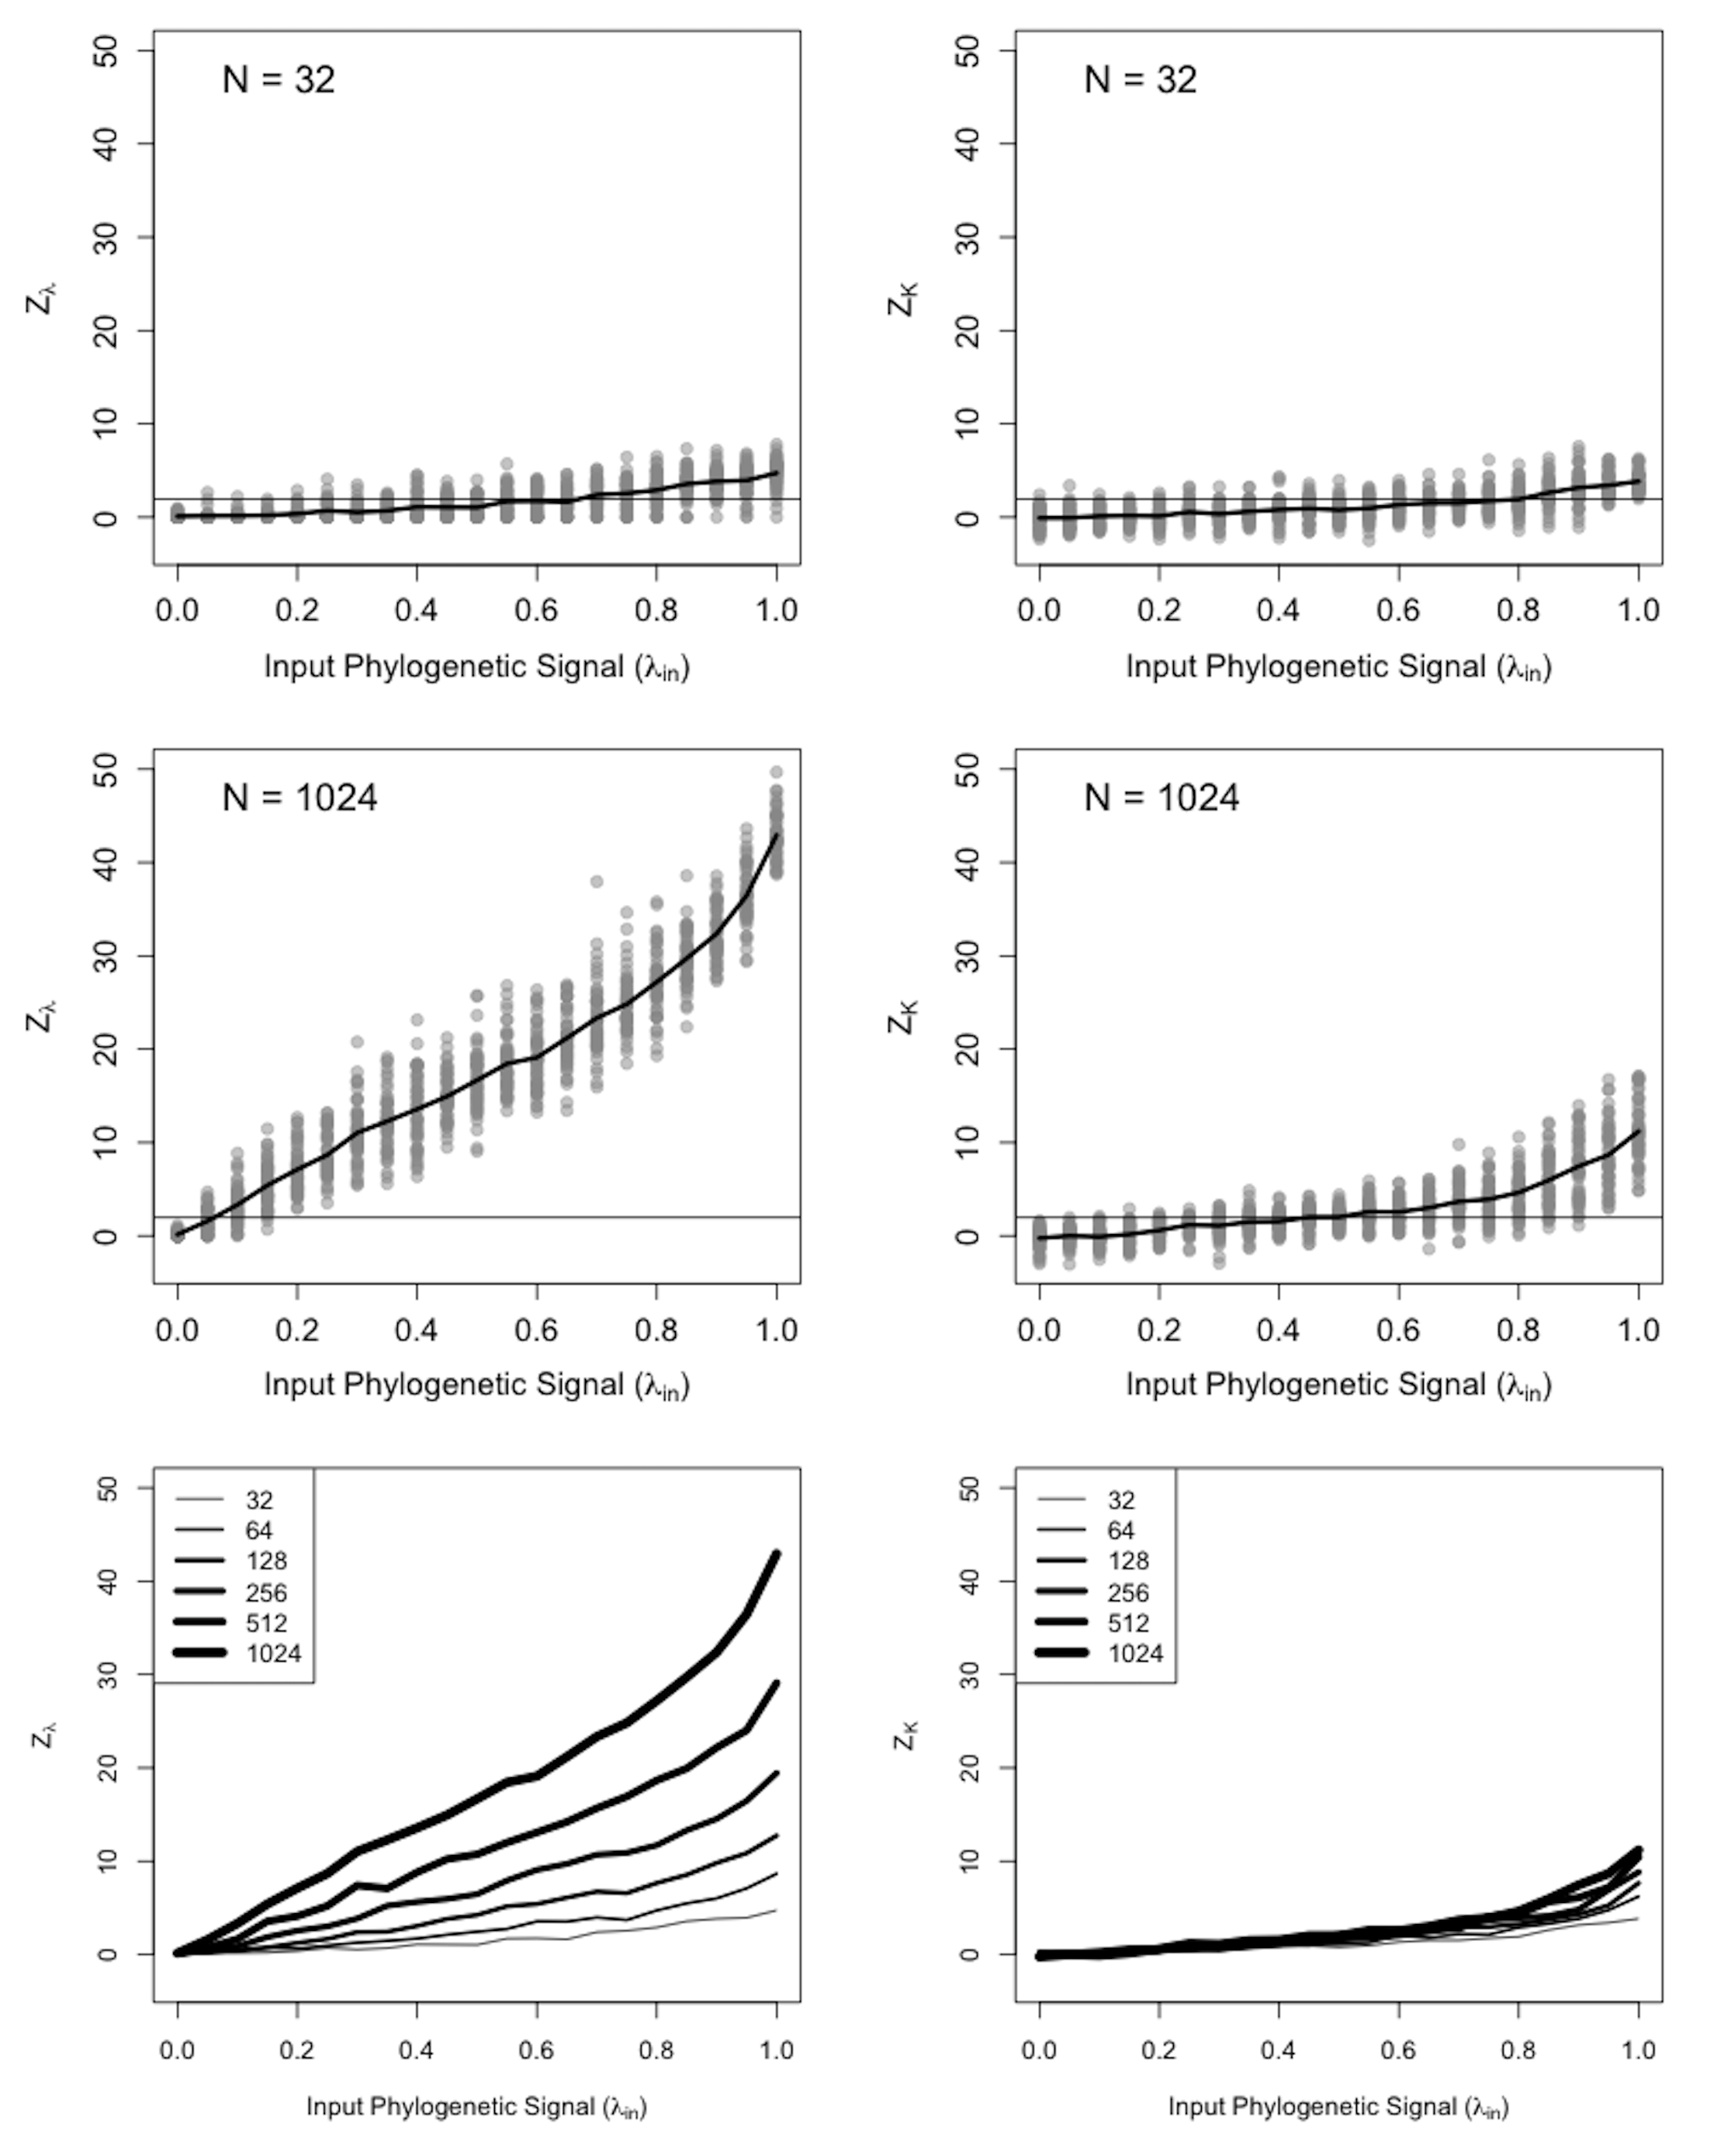
\includegraphics[width=0.95\linewidth]{fig.S1}

\textbf{Figure S1}. Response of effect sizes \(Z_{\lambda}\) and \(Z_K\)
to increasing strength of Brownian motion for pure-birth trees.

\newpage

\hypertarget{simulations-on-pectinate-phylogenies}{%
\subsection{Simulations on Pectinate
Phylogenies}\label{simulations-on-pectinate-phylogenies}}

Results from simulations on pectinate phylogenies largely mirrored those
found on pure-birth trees. For \(\hat{\lambda}\), the mean value
increased with increasing input signal, but was negatively biased, and
was less than the input value across most of its range (Fig. S2: black
line). Additionally, the precision of \(\hat{\lambda}\) varied with
differing input levels, with the greatest variation found at
intermediate values of \(\lambda\) (Fig. S2 red line). Finally, the
distribution of \(\hat{\lambda}\) was not normal, and became more skewed
at more extreme values of \(\lambda\) (Fig. S2 blue line). \hfill\break

For \emph{K}, mean values increased with increasing phylogenetic signal,
though as was found with pure-birth trees, the increase was nonlinear
(Fig. S3 black line). Likewise, variation increased with increasing
phylogenetic signal (Fig. S3 red line), though the distribution of
\emph{K} was more normally distributed throughout its range, and across
different tree sizes, as compared with \(\hat{\lambda}\), though there
was some slight skew for high input levels of phylogenetic signal on
large phylogenies (Fig. S3 blue line). \hfill\break

With respect to effect sizes, both \(Z_{\lambda}\) and \(Z_K\) increased
with increasing input phylogenetic signal, but \(\hat{\lambda}\) was
strongly affected by tree size, whereas \(Z_K\) was more consistent
(Fig. S4). Also, \(Z_K\) increased more linearly with increasing levels
of phylogenetic signal, and its standard deviation across input signal
was more even across tree sizes, implying more consistent precision.

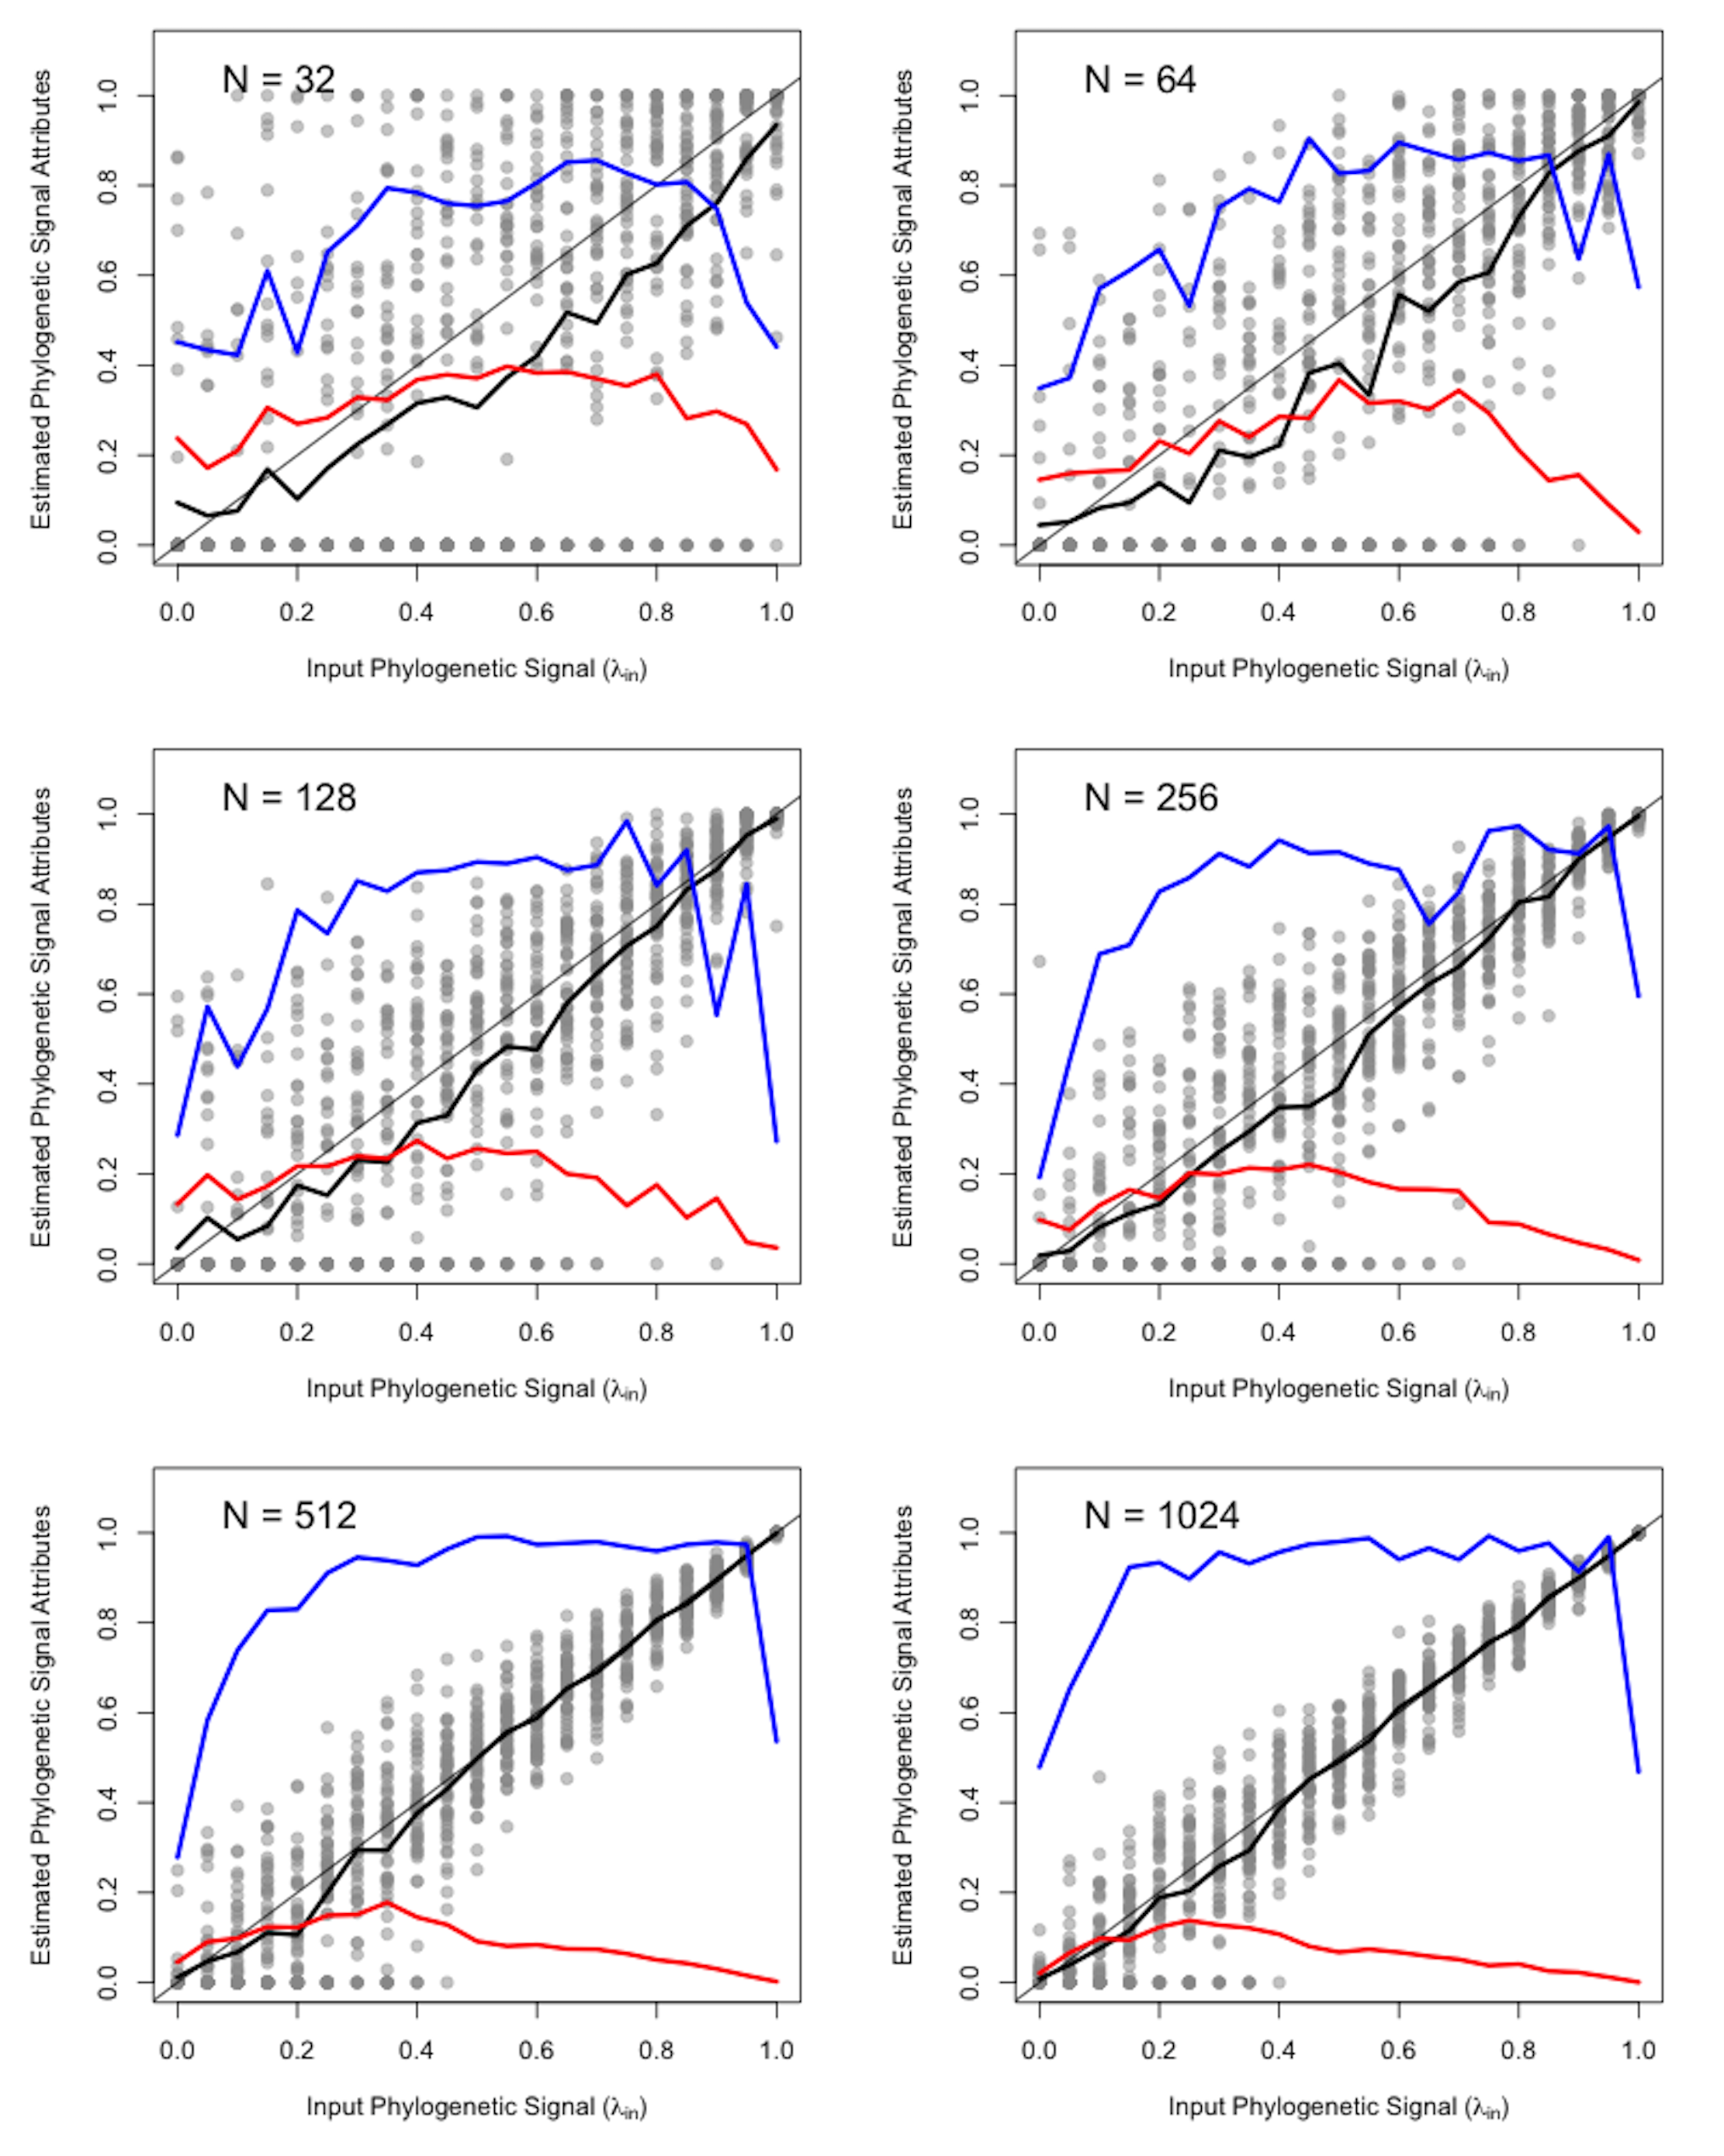
\includegraphics[width=0.95\linewidth]{fig.S2}

\textbf{Figure S2}. Response of Pagel's \(\lambda\) to increasing
strength of Brownian motion on pectinate trees. Gray line signifies the
1:1 line where the input value matches the estimate.At each input level,
the dark black line represents the empirically derived expected value
(mean) of \(\hat\lambda\), the red line is the standard deviation of
\(\hat\lambda\), and the blue line is Shapiro Wilks statistic of
\(\hat\lambda\) (\(W=1.0\) signifies normality, \(W< 1.0\) represent
skewed distributions).

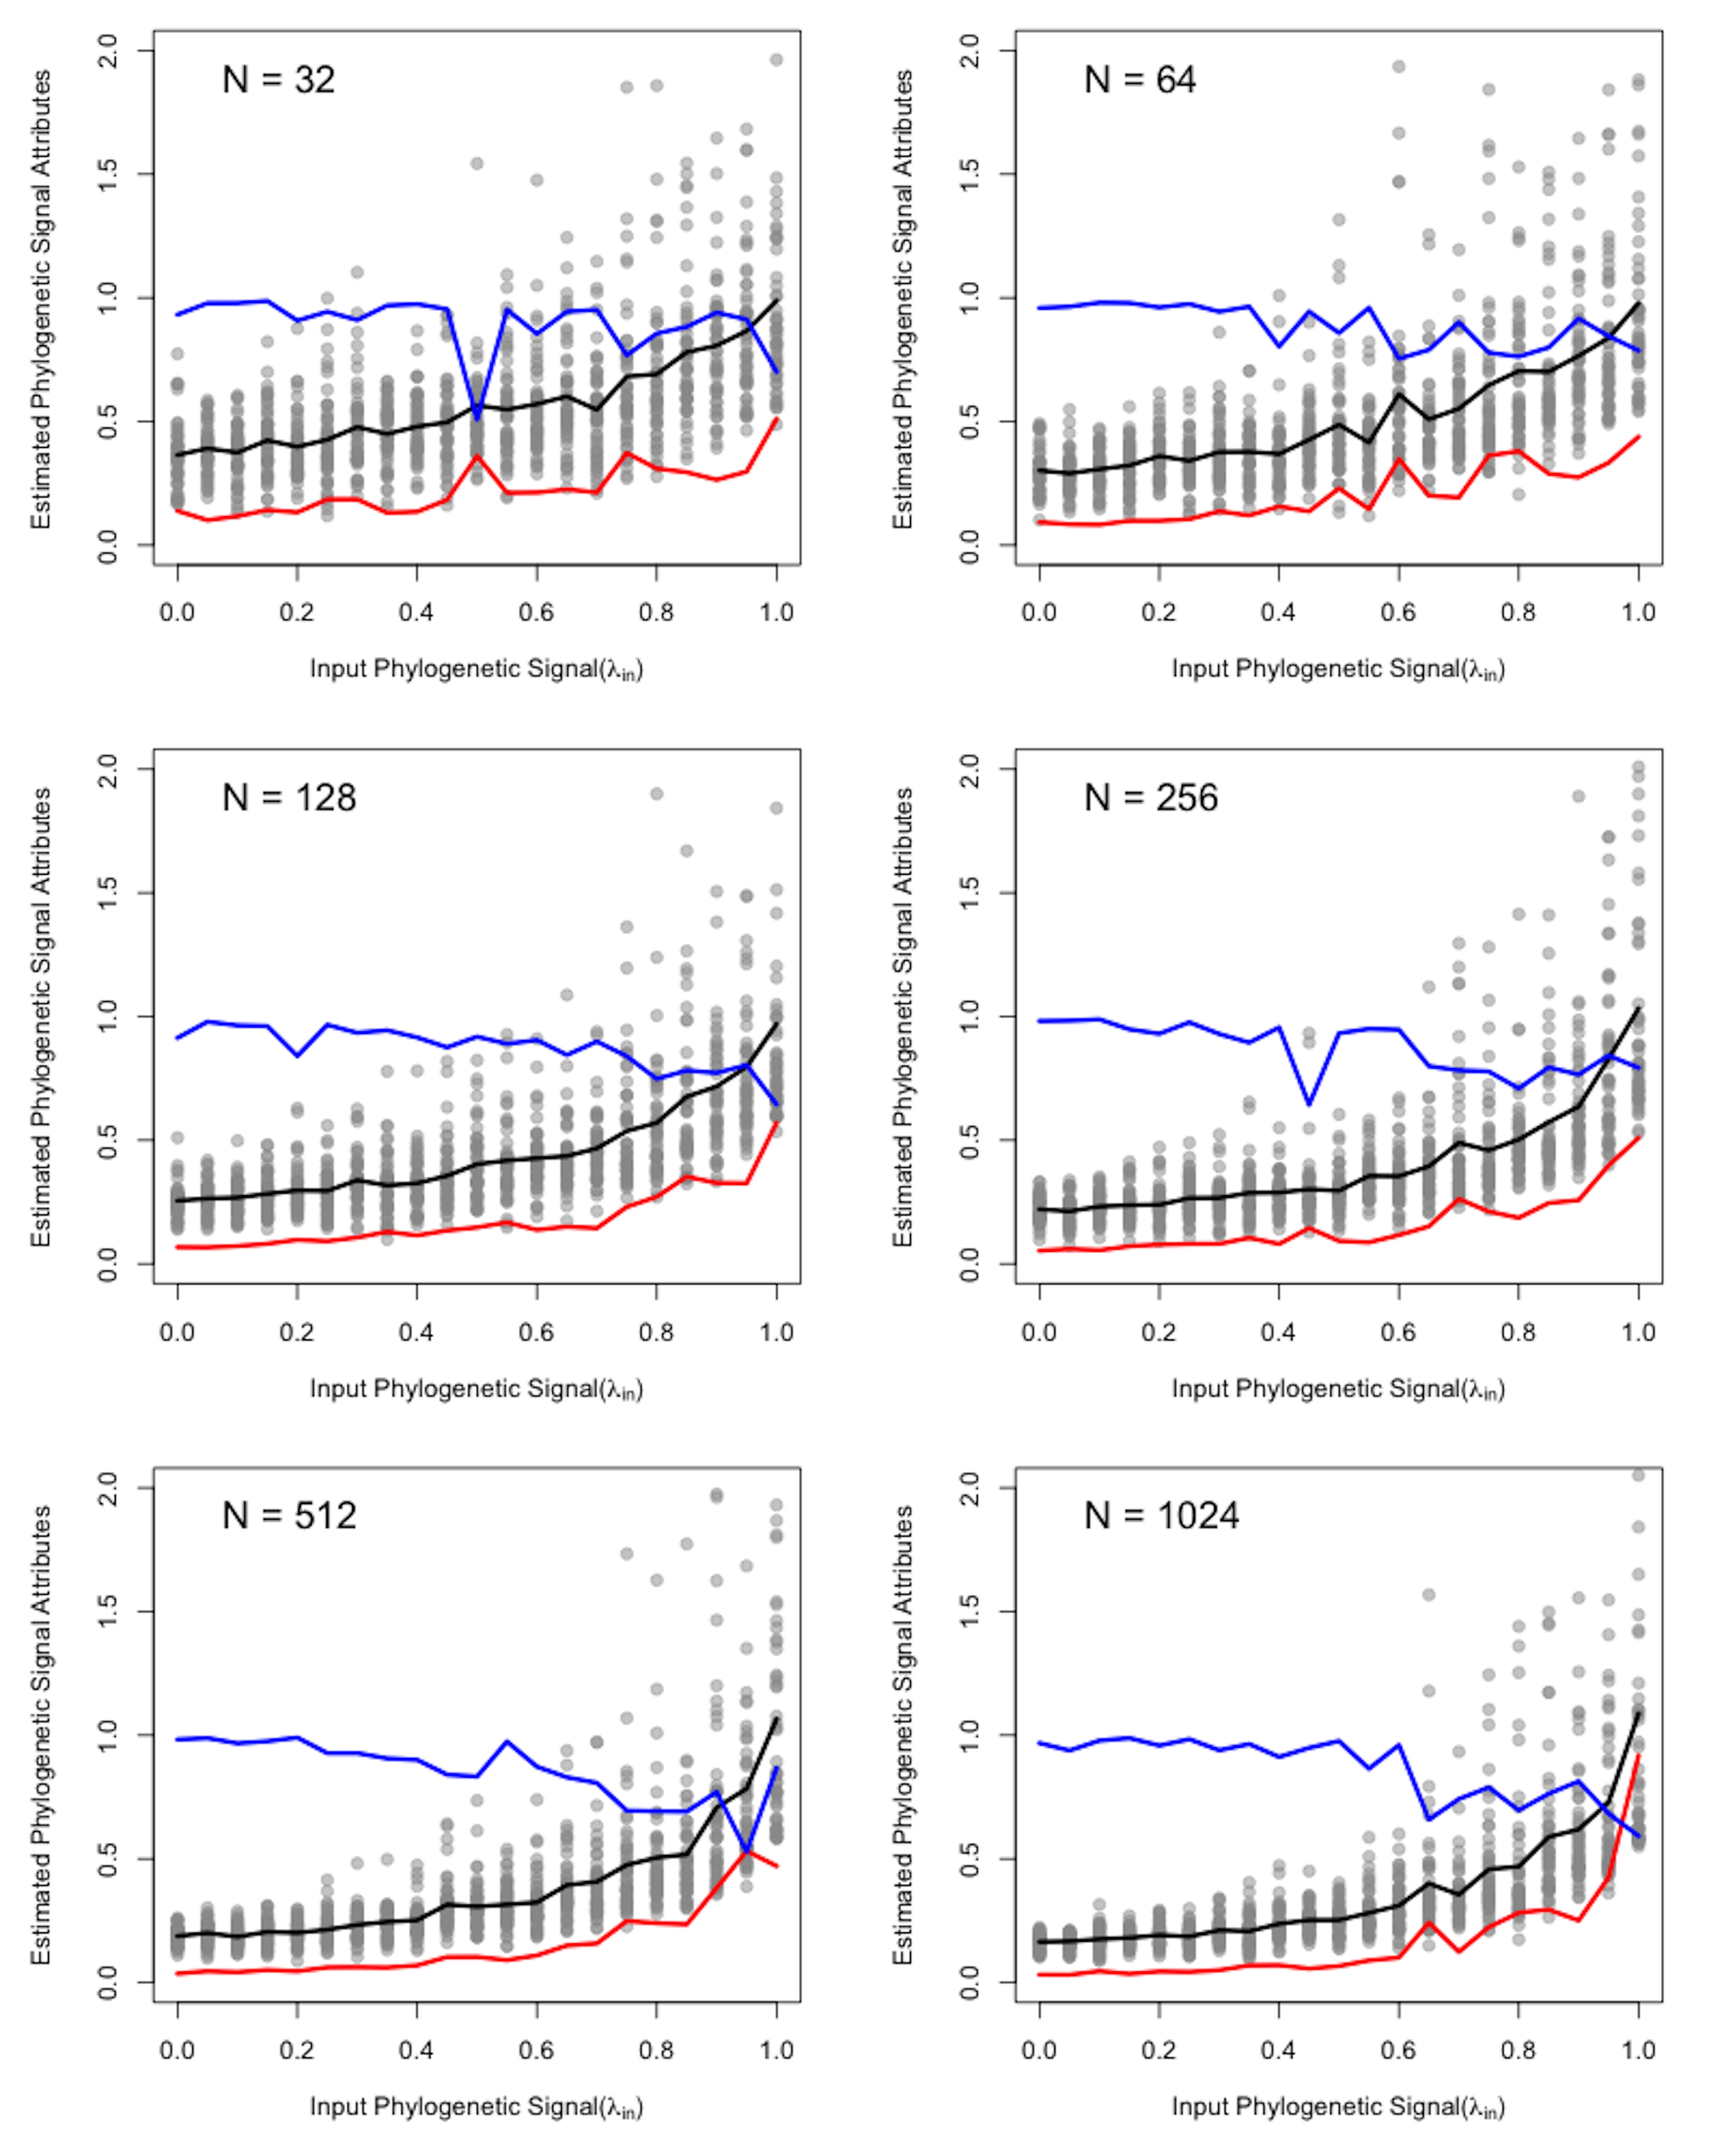
\includegraphics[width=0.95\linewidth]{fig.S3}

\textbf{Figure S3}. Response of Blomberg's \textit{K} to increasing
strength of Brownian motion on pectinate trees. At each input level, the
dark black line represents the empirically derived expected value (mean)
of \textit{K}, the red line is the standard deviation of \textit{K}, and
the blue line is Shapiro Wilks statistic of \textit{K} (\(W=1.0\)
signifies normality, \(W< 1.0\) represent skewed distributions).

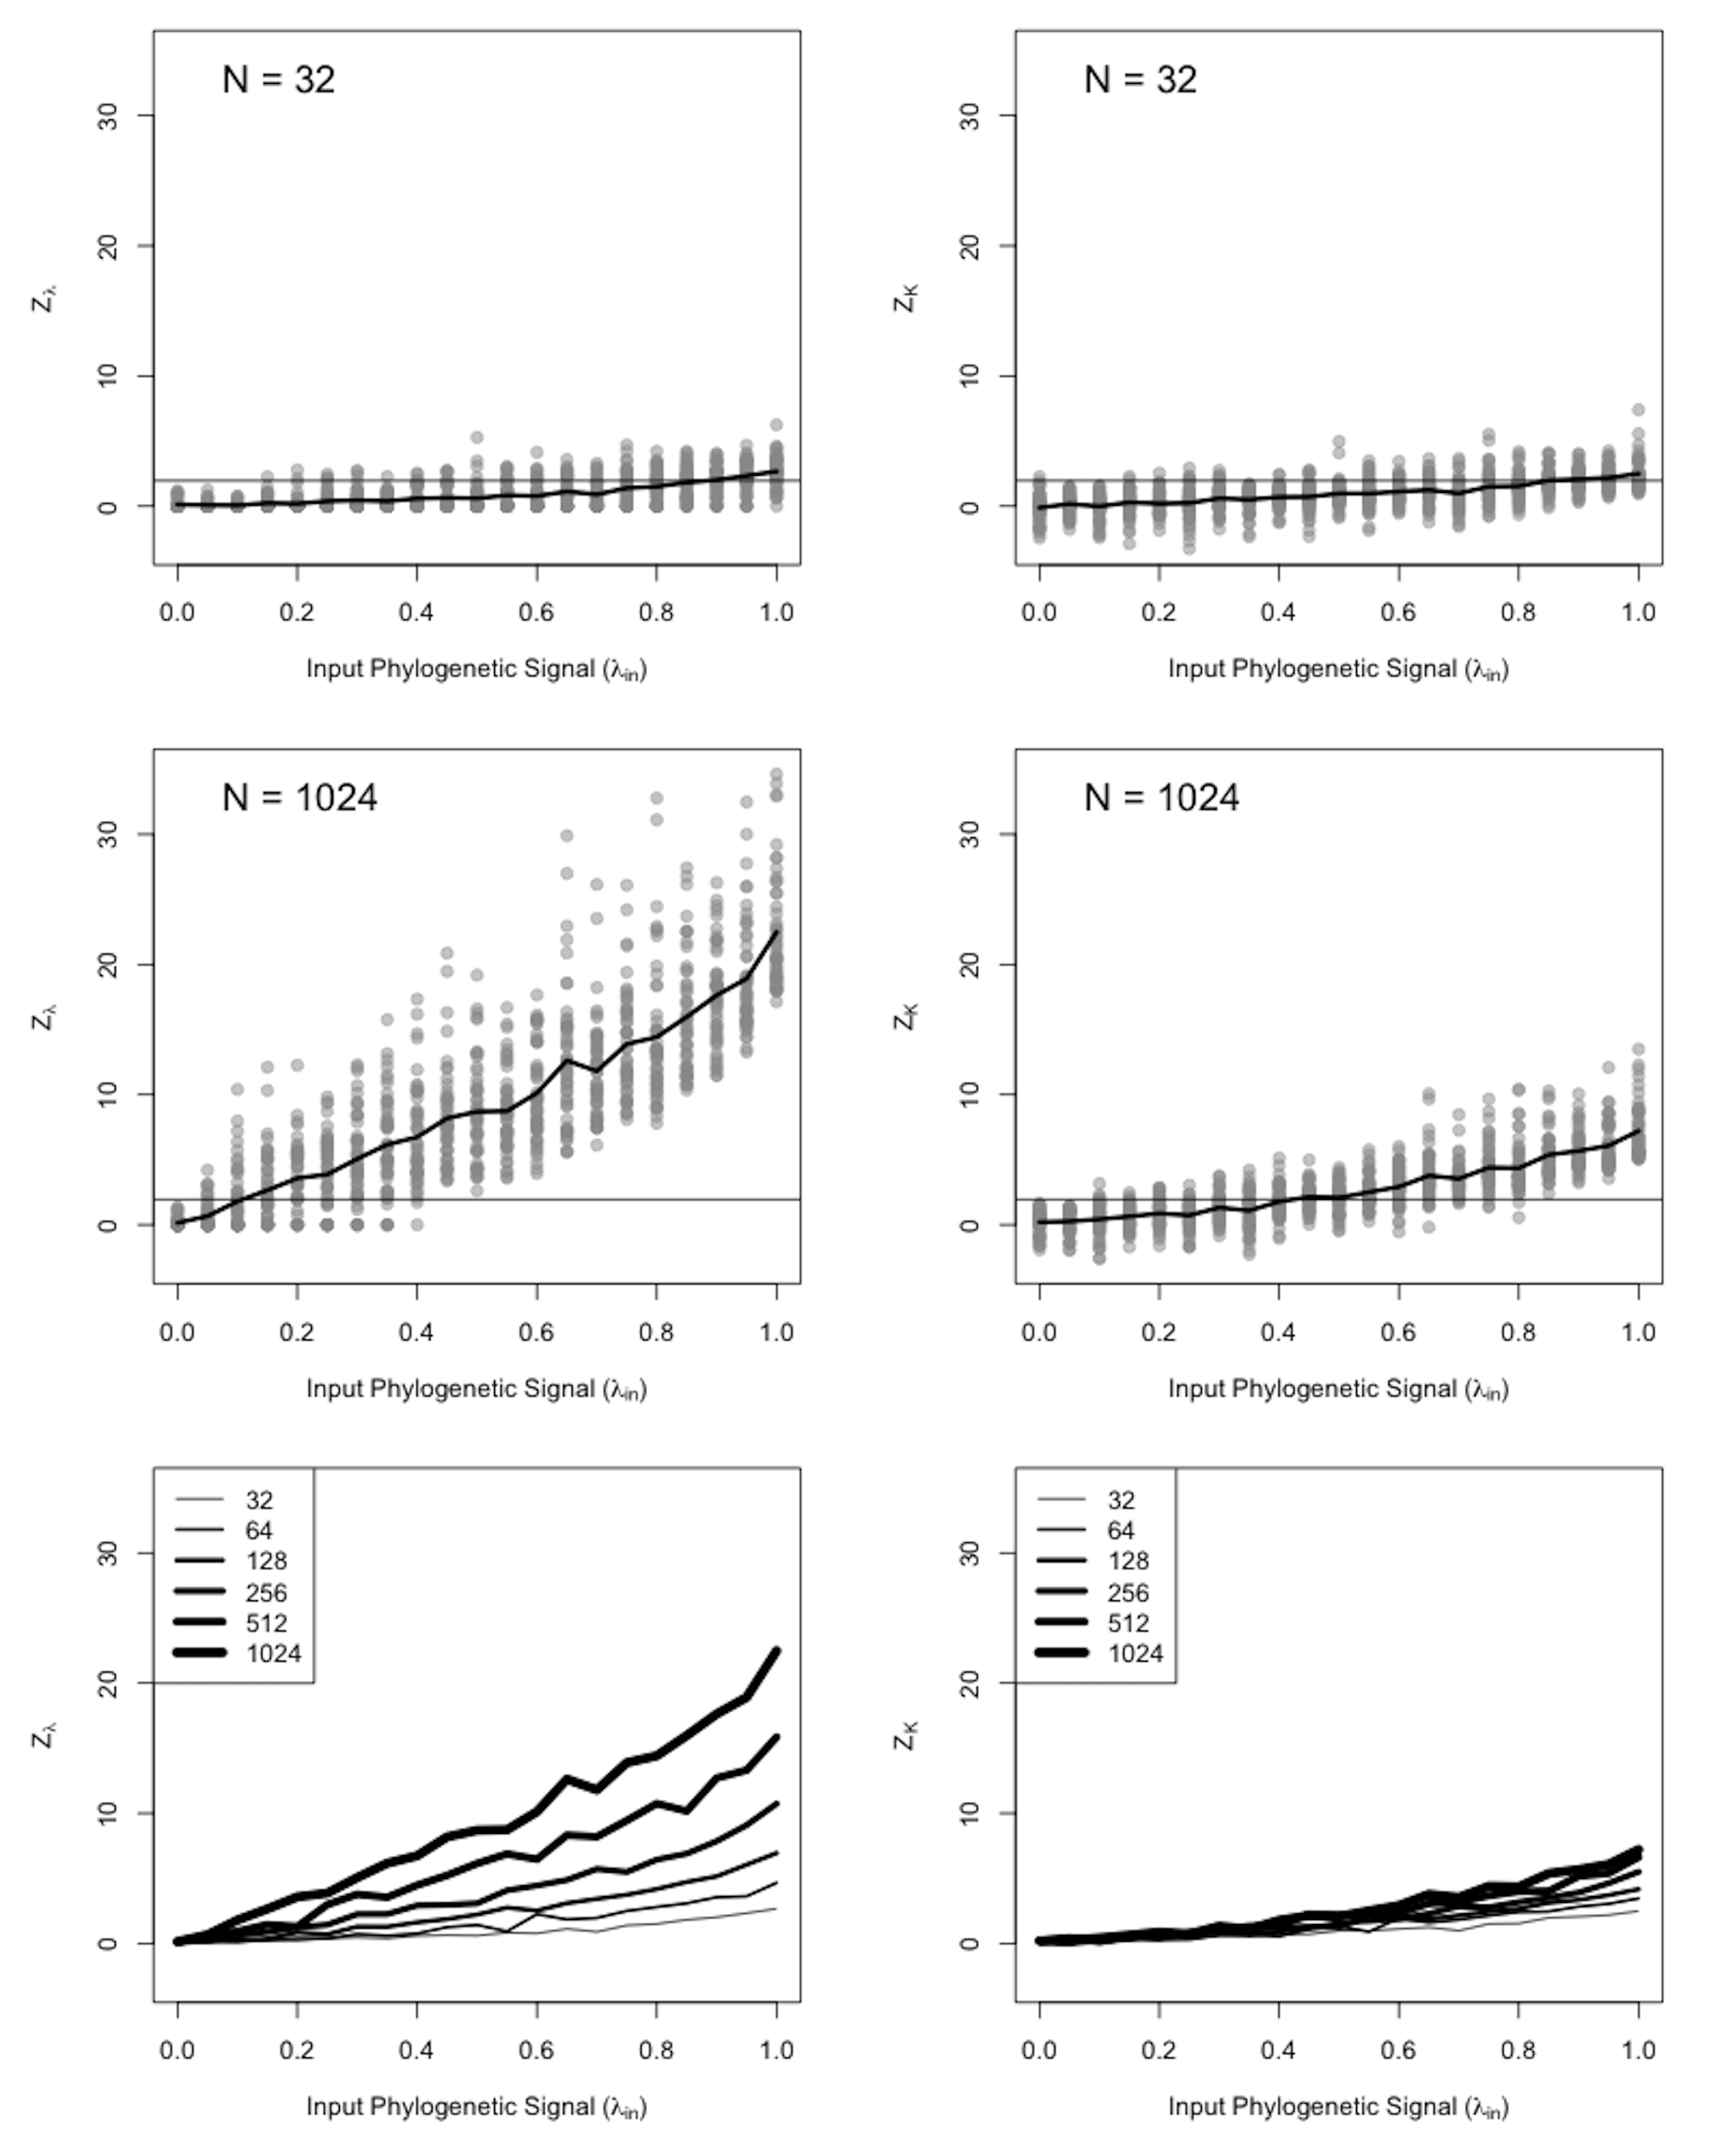
\includegraphics[width=0.95\linewidth]{fig.S4}

\textbf{Figure S4}. Response of effect sizes \(Z_{\lambda}\) and \(Z_K\)
to increasing strength of Brownian motion for pectinate trees.

\newpage

\hypertarget{simulations-on-balanced-phylogenies}{%
\subsection{Simulations on Balanced
Phylogenies}\label{simulations-on-balanced-phylogenies}}

Results from simulations on balanced phylogenies also mirrored those
found on pure-birth trees. For \(\hat{\lambda}\), the mean value
increased with increasing input signal, but was negatively biased, and
was less than the input value across most of its range (Fig. S5: black
line). Additionally, the precision of \(\hat{\lambda}\) varied with
differing input levels, with the greatest variation found at
intermediate values of \(\lambda\) (Fig. S5 red line). Finally, the
distribution of \(\hat{\lambda}\) was not normal, and became more skewed
at more extreme values of \(\lambda\) (Fig. S5 blue line). \hfill\break

For \emph{K}, mean values increased with increasing phylogenetic signal,
though as was found with pure-birth trees, the increase was nonlinear
(Fig. S6 black line). Likewise, variation increased with increasing
phylogenetic signal (Fig. S6 red line), though the distribution of
\emph{K} was more normally distributed throughout its range, and across
different tree sizes, as compared with \(\hat{\lambda}\), though there
was some slight skew for high input levels of phylogenetic signal on
large phylogenies (Fig. S6 blue line). \hfill\break

With respect to effect sizes, both \(Z_{\lambda}\) and \(Z_K\) increased
with increasing input phylogenetic signal, but \(\hat{\lambda}\) was
strongly affected by tree size (fig.~S7). Also, \(Z_K\) increased more
linearly with increasing levels of phylogenetic signal, though there was
a slight effect of tree size with balanced phylogenies. But as before,
its standard deviation across input signal was more even across tree
sizes, implying more consistent precision.

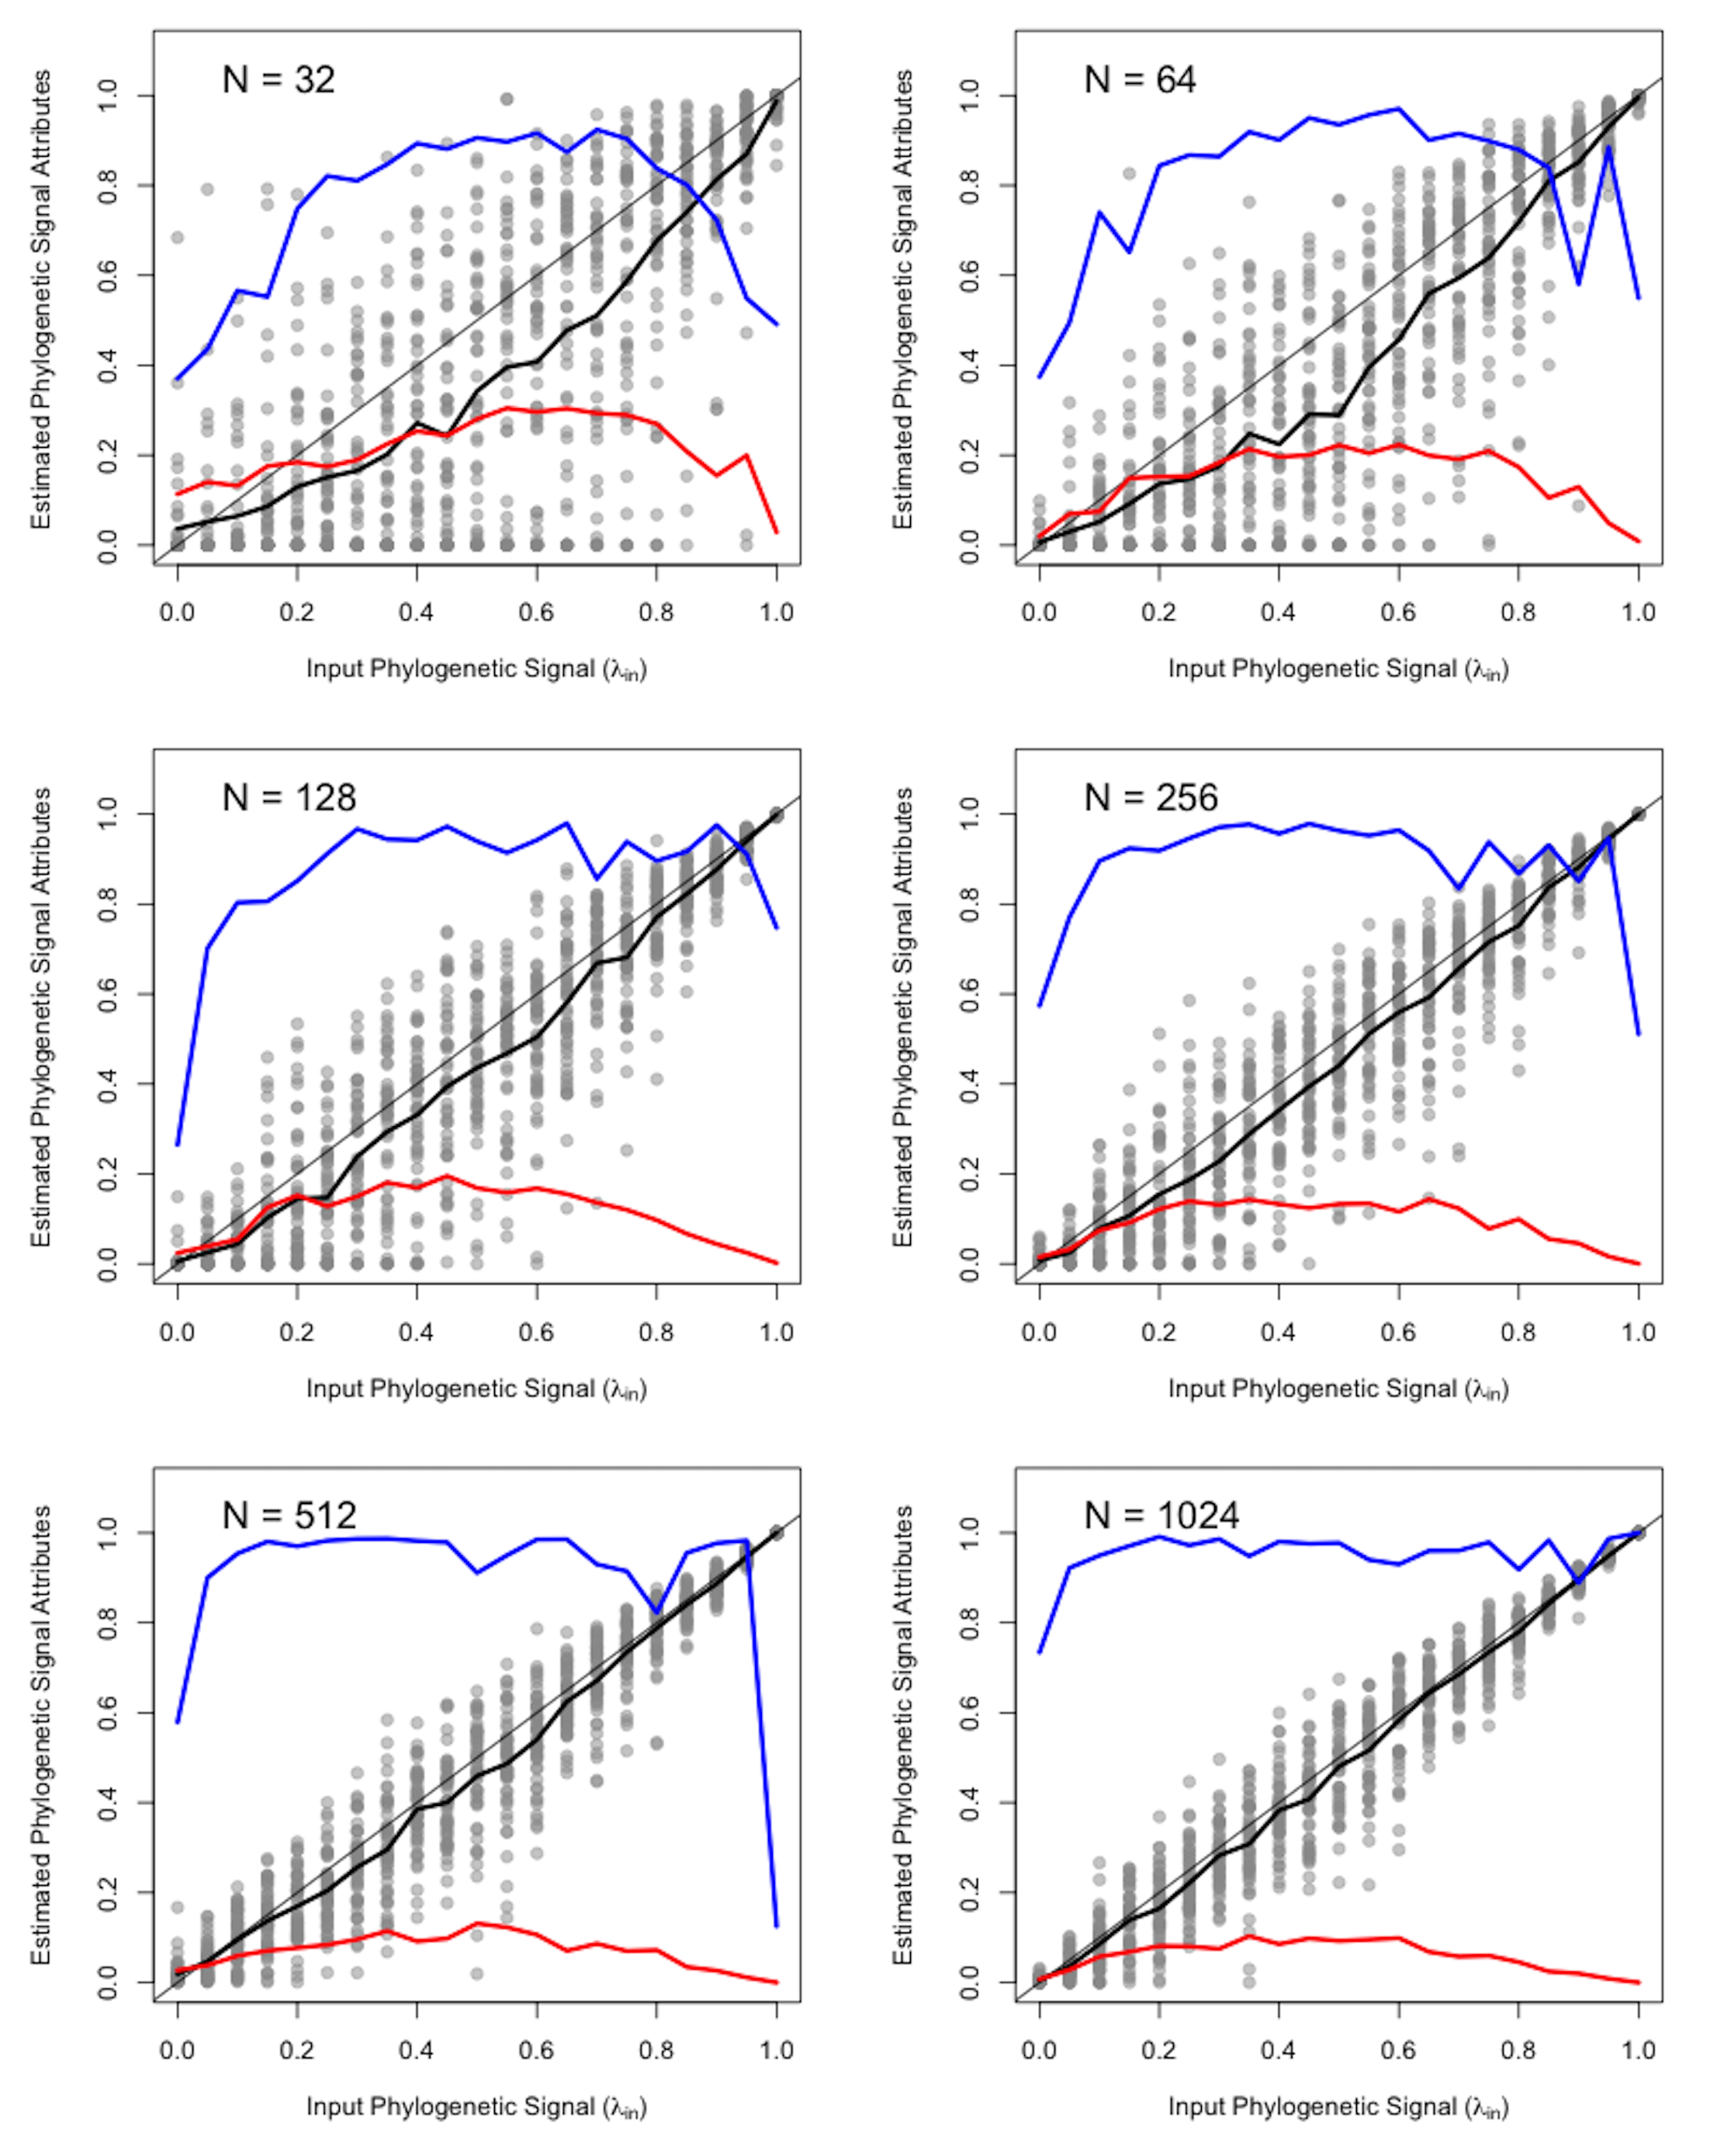
\includegraphics[width=0.95\linewidth]{fig.S5}

\textbf{Figure S5}. Response of Pagel's \(\lambda\) to increasing
strength of Brownian motion on balanced trees. Gray line signifies the
1:1 line where the input value matches the estimate. At each input
level, the dark black line represents the empirically derived expected
value (mean) of \(\hat\lambda\), the red line is the standard deviation
of \(\hat\lambda\), and the blue line is Shapiro Wilks statistic of
\(\hat\lambda\) (\(W=1.0\) signifies normality, \(W< 1.0\) represent
skewed distributions).

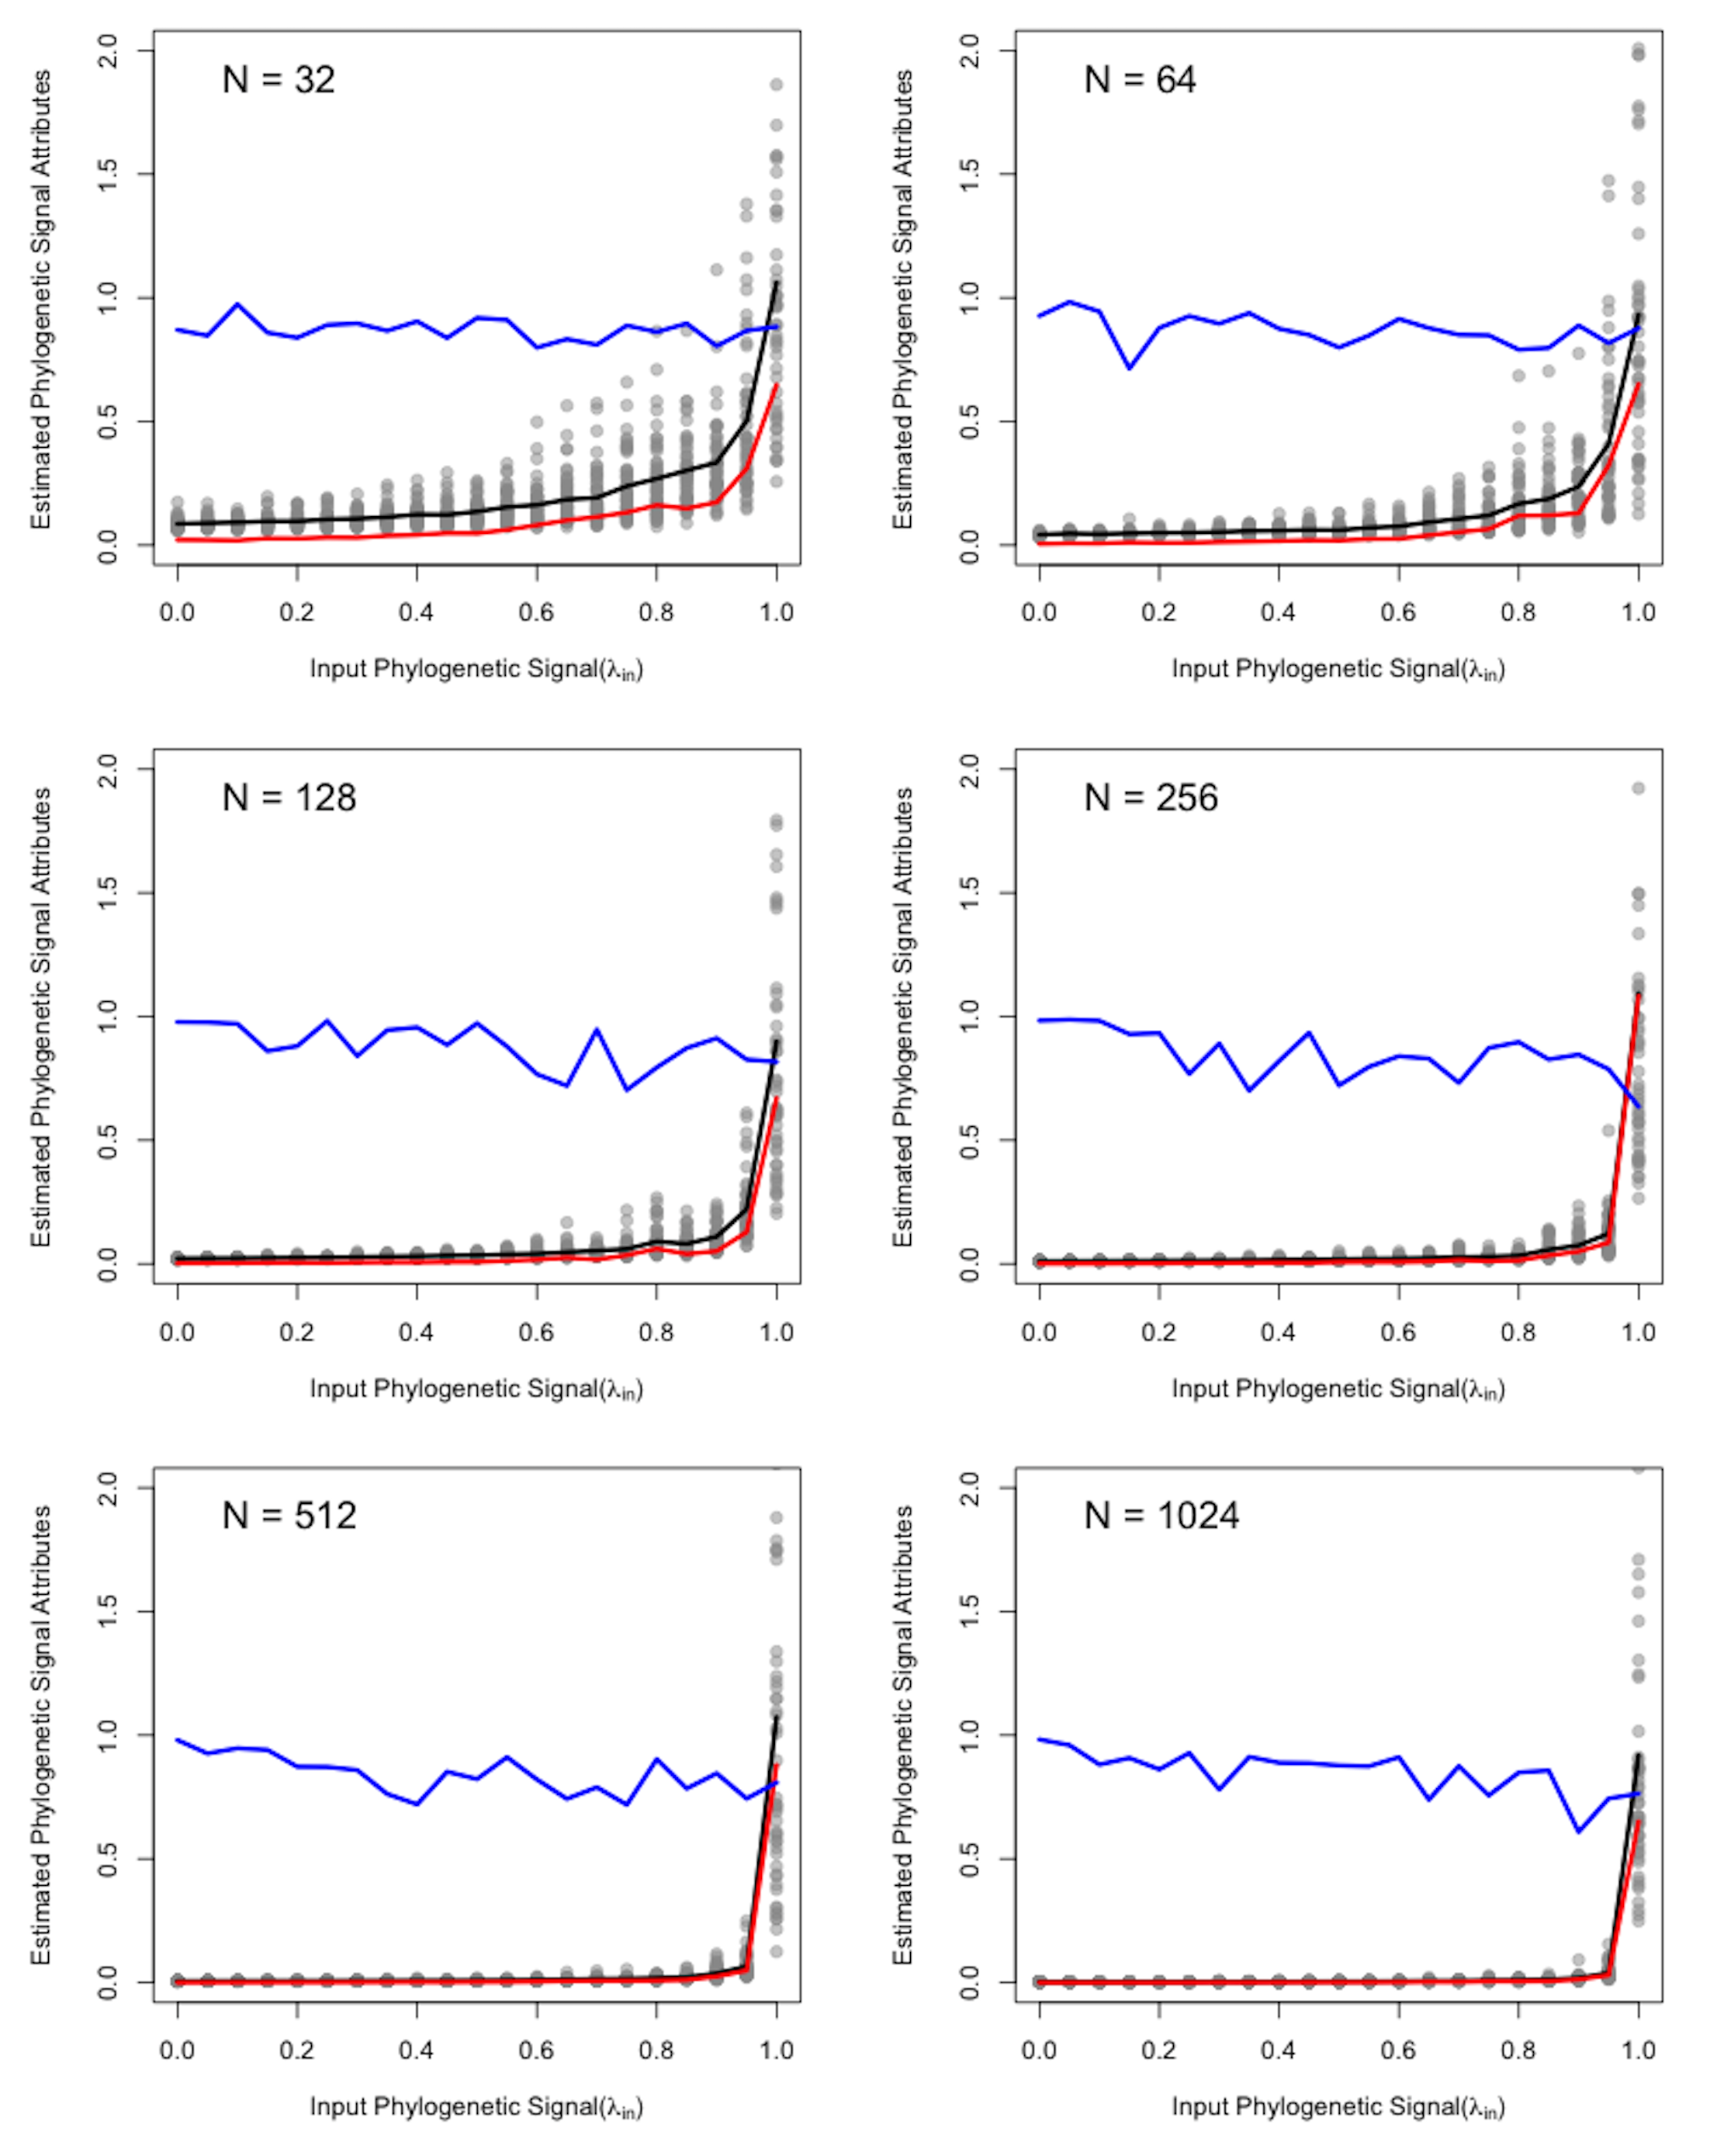
\includegraphics[width=0.95\linewidth]{fig.S6}

\textbf{Figure S6}. Response of Blomberg's \textit{K} to increasing
strength of Brownian motion on balanced trees. At each input level, the
dark black line represents the empirically derived expected value (mean)
of \textit{K}, the red line is the standard deviation of \textit{K}, and
the blue line is Shapiro Wilks statistic of \textit{K} (\(W=1.0\)
signifies normality, \(W< 1.0\) represent skewed distributions).

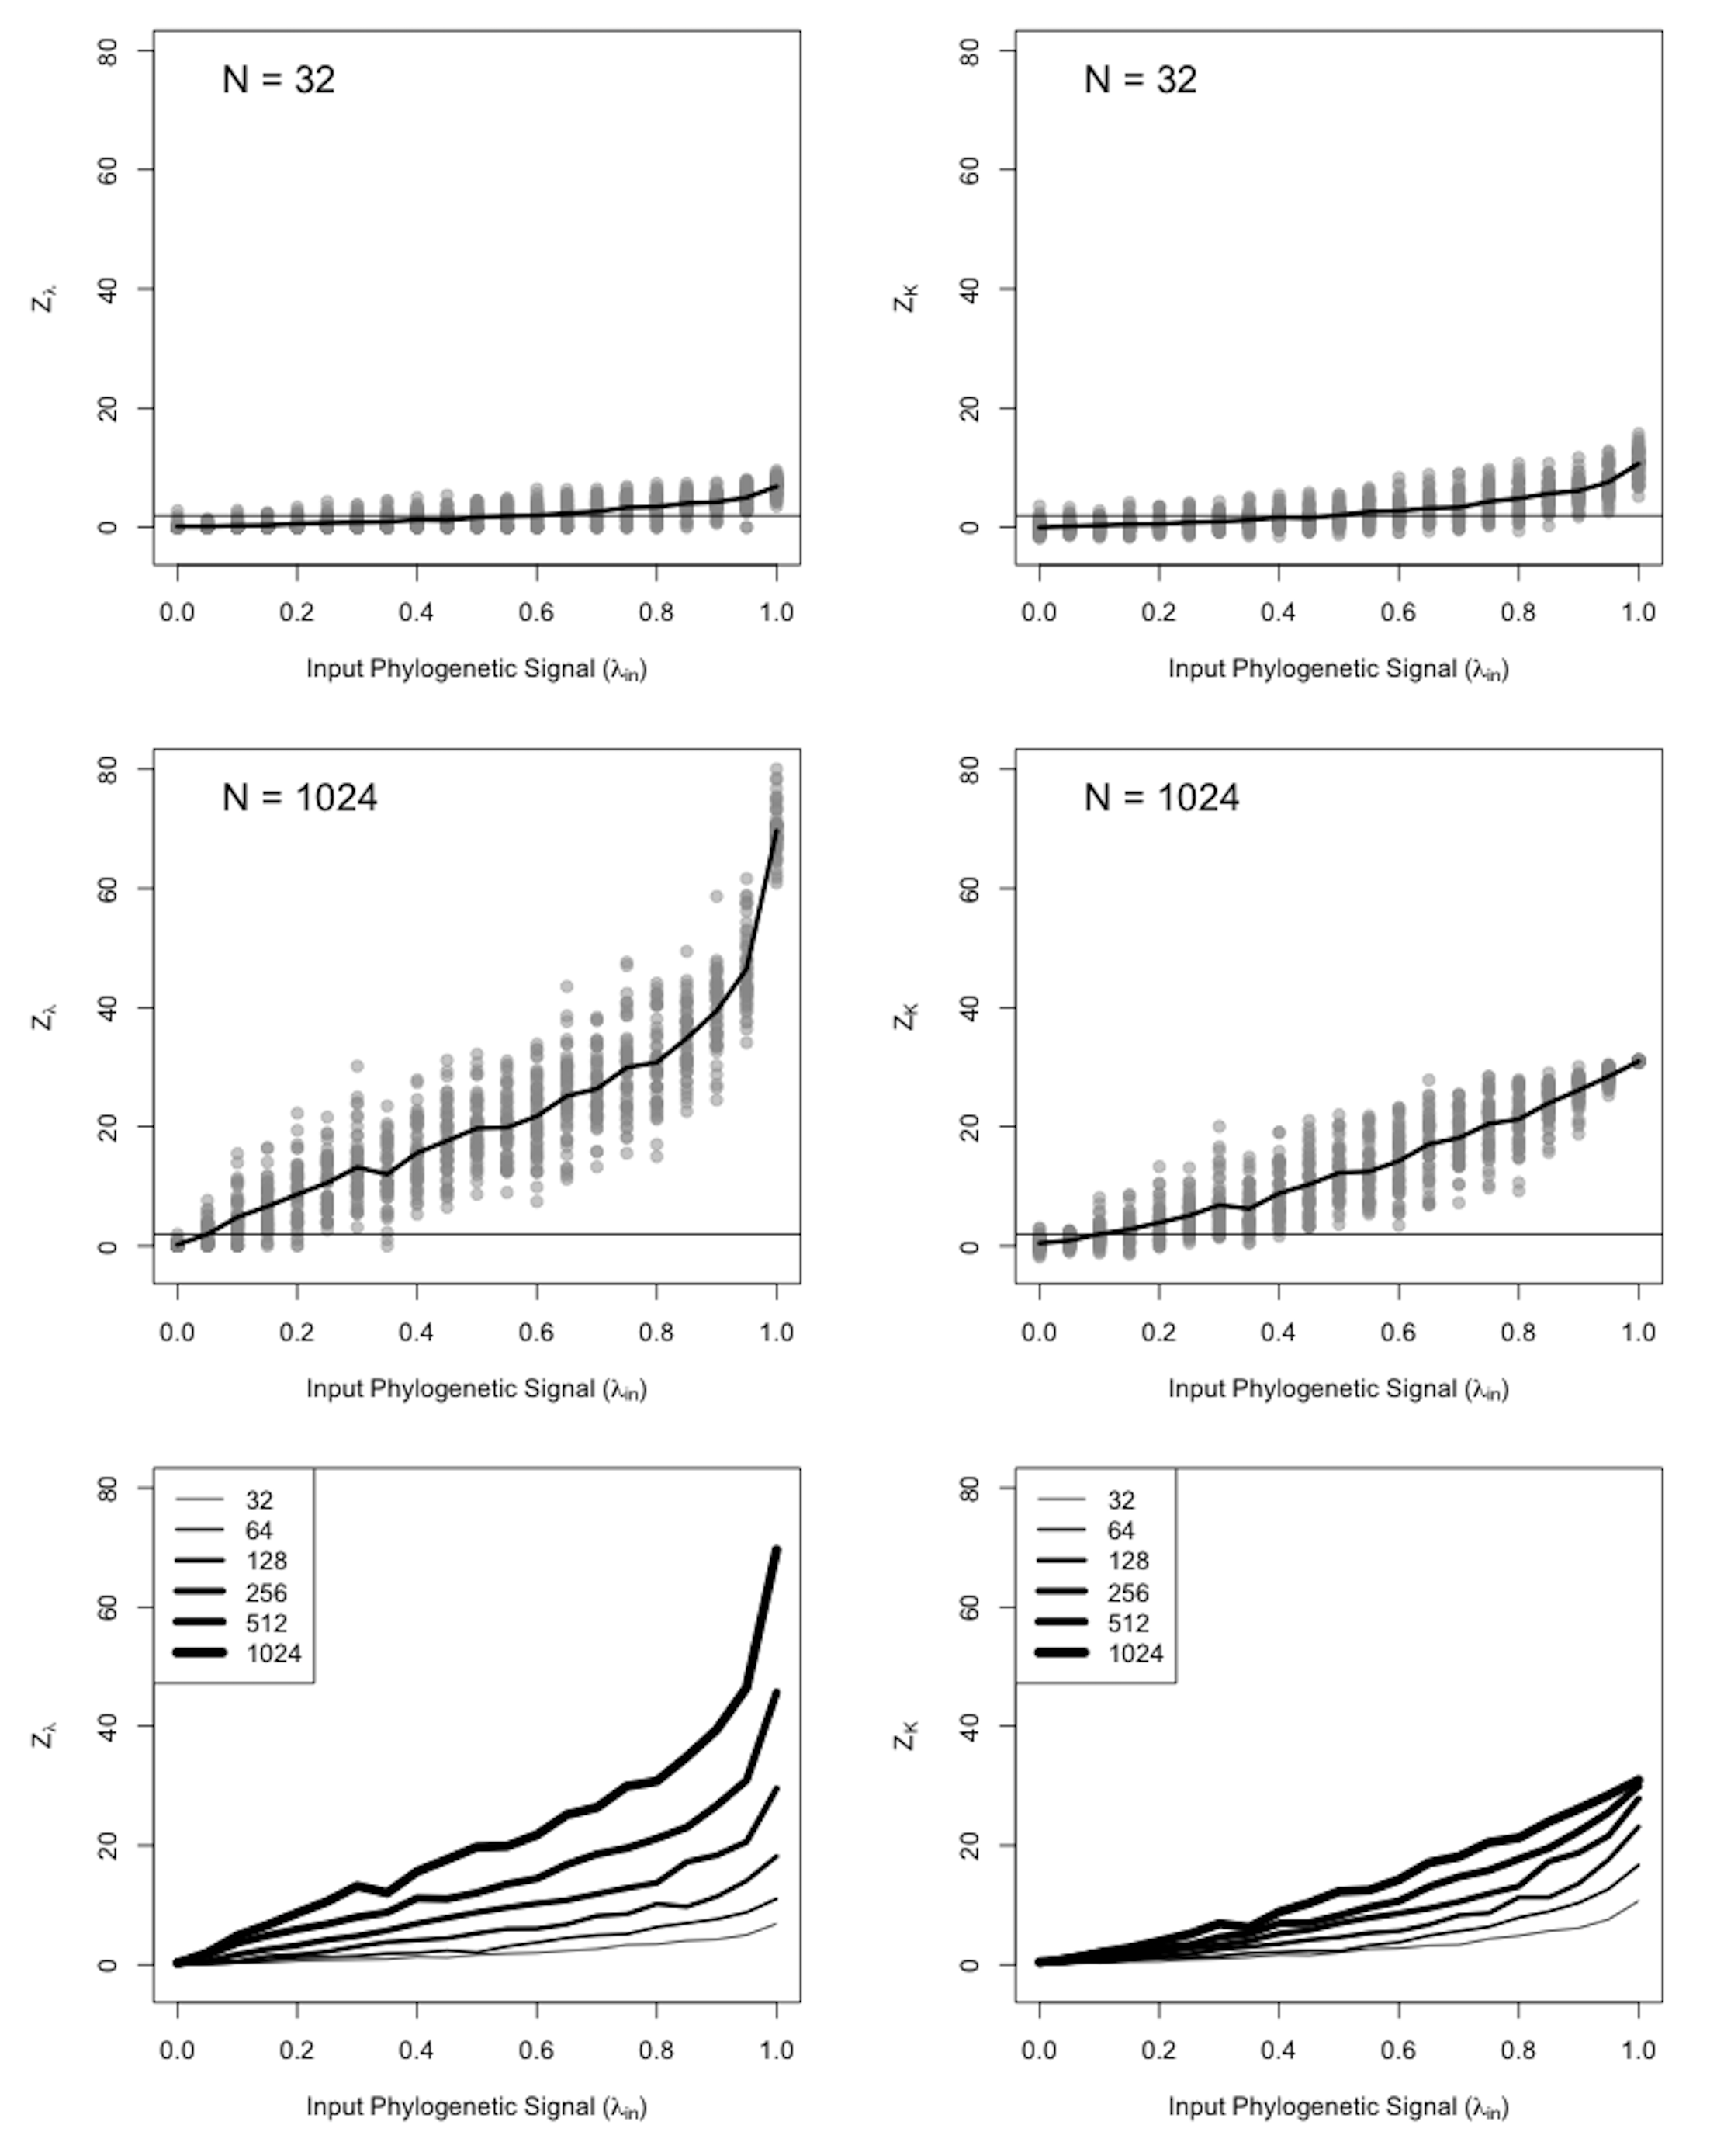
\includegraphics[width=0.95\linewidth]{fig.S7}

\textbf{Figure S7}. Response of effect sizes \(Z_{\lambda}\) and \(Z_K\)
to increasing strength of Brownian motion for balanced trees.

\newpage

\hypertarget{simulations-on-phylogenies-containing-polytomies}{%
\subsection{Simulations on Phylogenies Containing
Polytomies}\label{simulations-on-phylogenies-containing-polytomies}}

We also investigaged the effect of unresolved phylogenies on estimates
of phylogenetic signal by adjusting pure-birth trees to have 20\%
collapsed nodes, following the procedures of (1). Results from
simulations on phylogenies containing polytomies mirrored those found on
fully resolved trees. For \(\hat{\lambda}\), the mean value increased
with increasing input signal, but was negatively biased, and was less
than the input value across most of its range (Fig. S8: black line).
Additionally, the precision of \(\hat{\lambda}\) varied with differing
input levels, with the greatest variation found at intermediate values
of \(\lambda\) (Fig. S8 red line). Finally, the distribution of
\(\hat{\lambda}\) was not normal, and became more skewed at more extreme
values of \(\lambda\) (Fig. S8 blue line). \hfill\break

For \emph{K}, mean values increased with increasing phylogenetic signal,
though as was found with pure-birth trees, the increase was nonlinear
(Fig. S9 black line). Likewise, variation increased with increasing
phylogenetic signal (Fig. S9 red line), though the distribution of
\emph{K} was more normally distributed throughout its range, and across
different tree sizes, as compared with \(\hat{\lambda}\) (Fig. S9 blue
line). \hfill\break

With respect to effect sizes, both \(Z_{\lambda}\) and \(Z_K\) increased
with increasing input phylogenetic signal, but \(\hat{\lambda}\) was
strongly affected by tree size, whereas \(Z_K\) was more consistent
(Fig. S10). Also, \(Z_K\) increased more linearly with increasing levels
of phylogenetic signal, and its standard deviation across input signal
was more even across tree sizes, implying more consistent precision.
Thus, polytomies do not exert an appreciable effect on \(Z_K\).

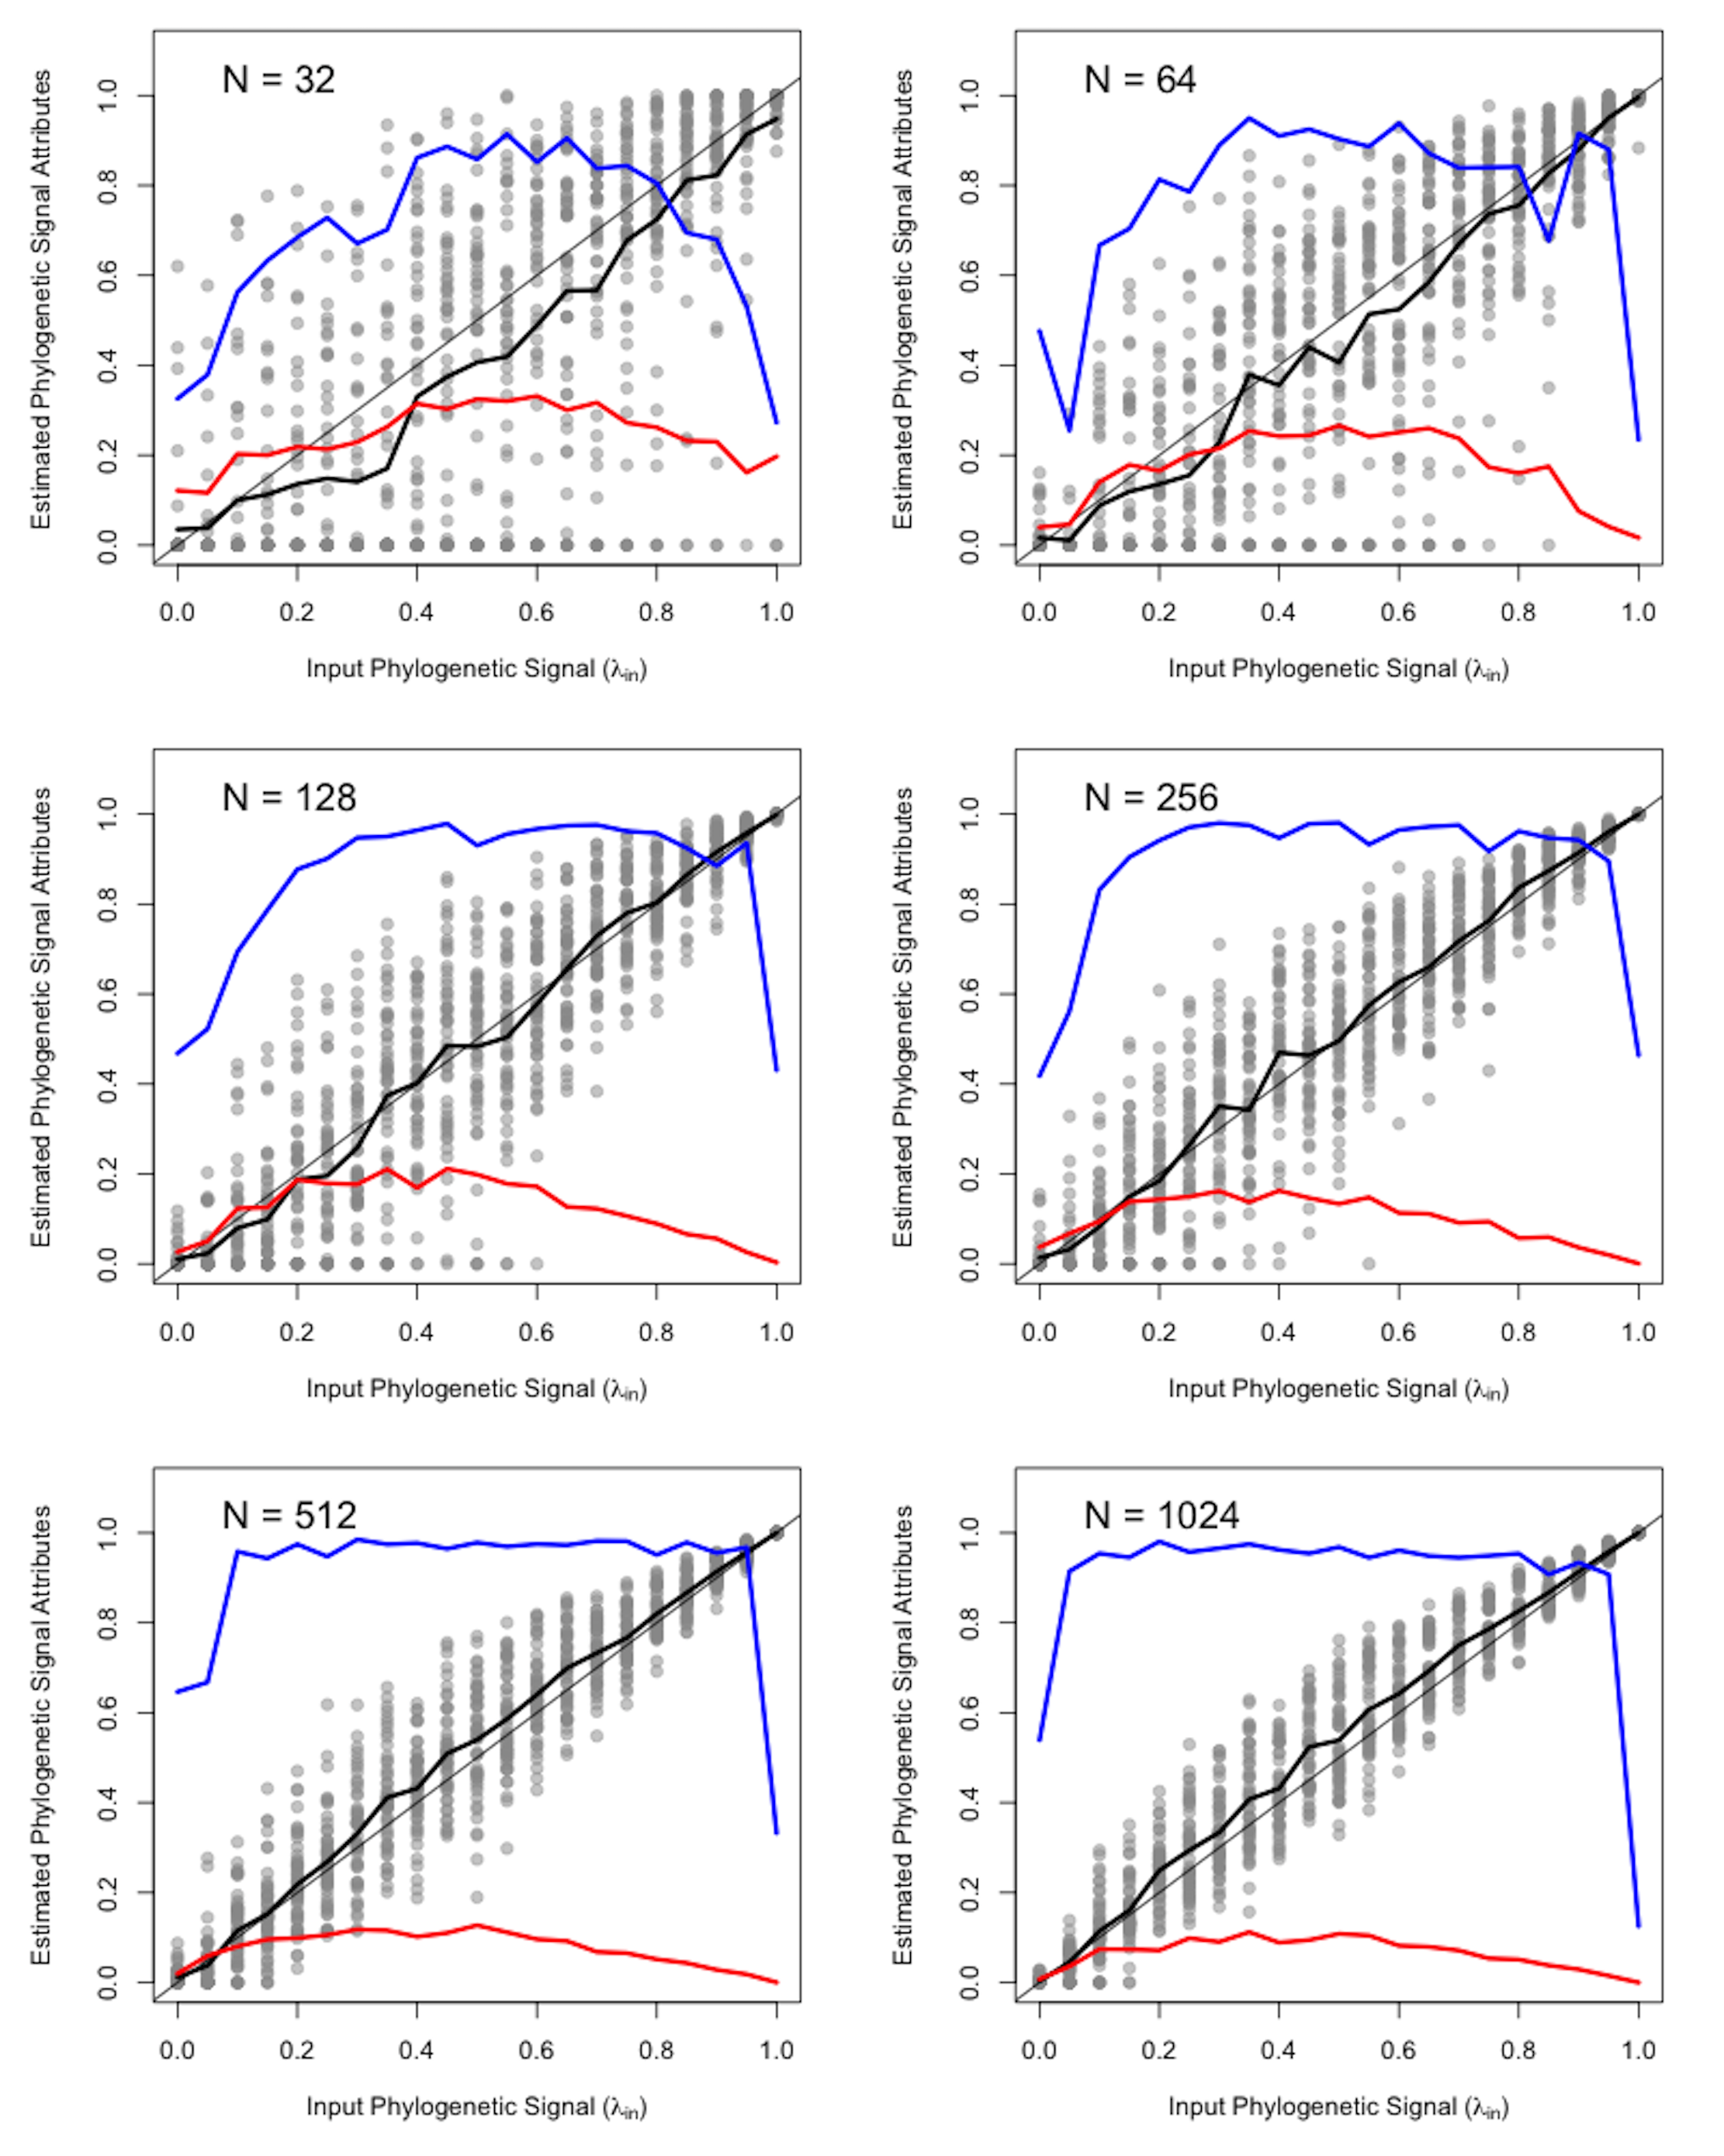
\includegraphics[width=0.95\linewidth]{fig.S8}

\textbf{Figure S8}. Response of Pagel's \(\lambda\) to increasing
strength of Brownian motion on pure-birth trees containing polytomies.
Gray line signifies the 1:1 line where the input value matches the
estimate. At each input level, the dark black line represents the
empirically derived expected value (mean) of \(\hat\lambda\), the red
line is the standard deviation of \(\hat\lambda\), and the blue line is
Shapiro Wilks statistic of \(\hat\lambda\) (\(W=1.0\) signifies
normality, \(W< 1.0\) represent skewed distributions).

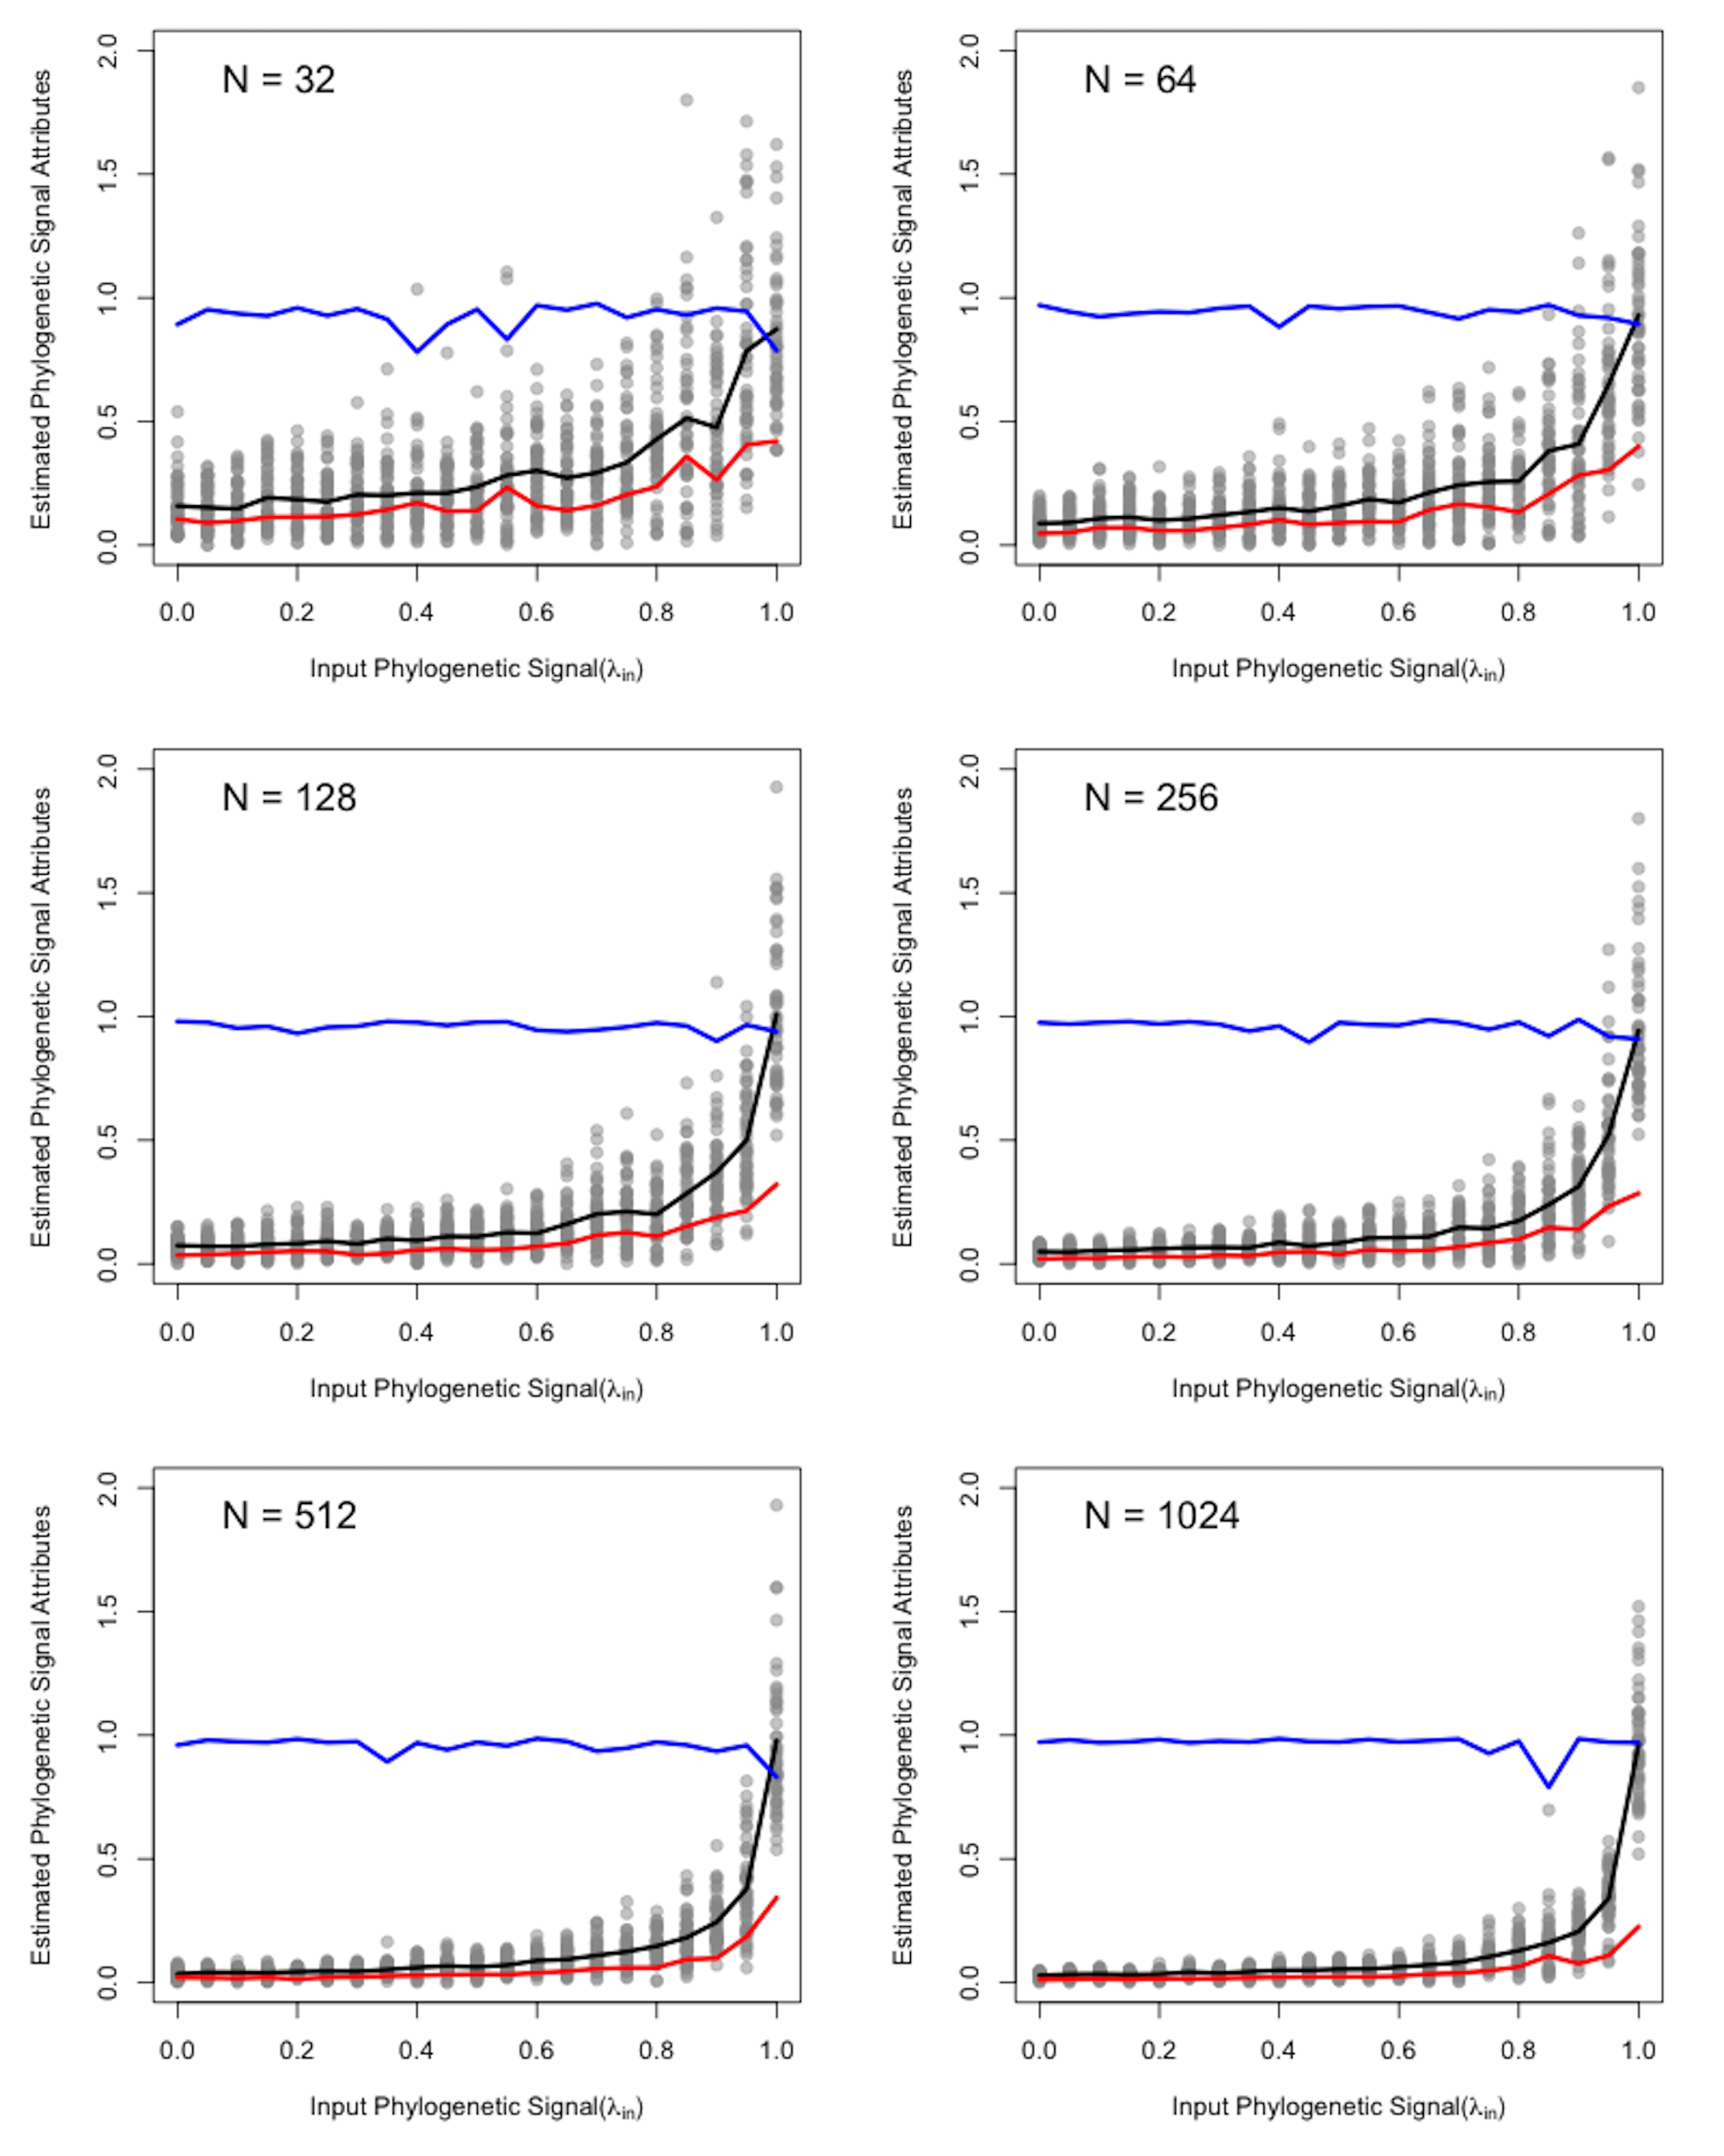
\includegraphics[width=0.95\linewidth]{fig.S9}

\textbf{Figure S9}. Response of Blomberg's \textit{K} to increasing
strength of Brownian motion on pure-birth trees containing polytomies.
At each input level, the dark black line represents the empirically
derived expected value (mean) of \textit{K}, the red line is the
standard deviation of \textit{K}, and the blue line is Shapiro Wilks
statistic of \textit{K} (\(W=1.0\) signifies normality, \(W< 1.0\)
represent skewed distributions).

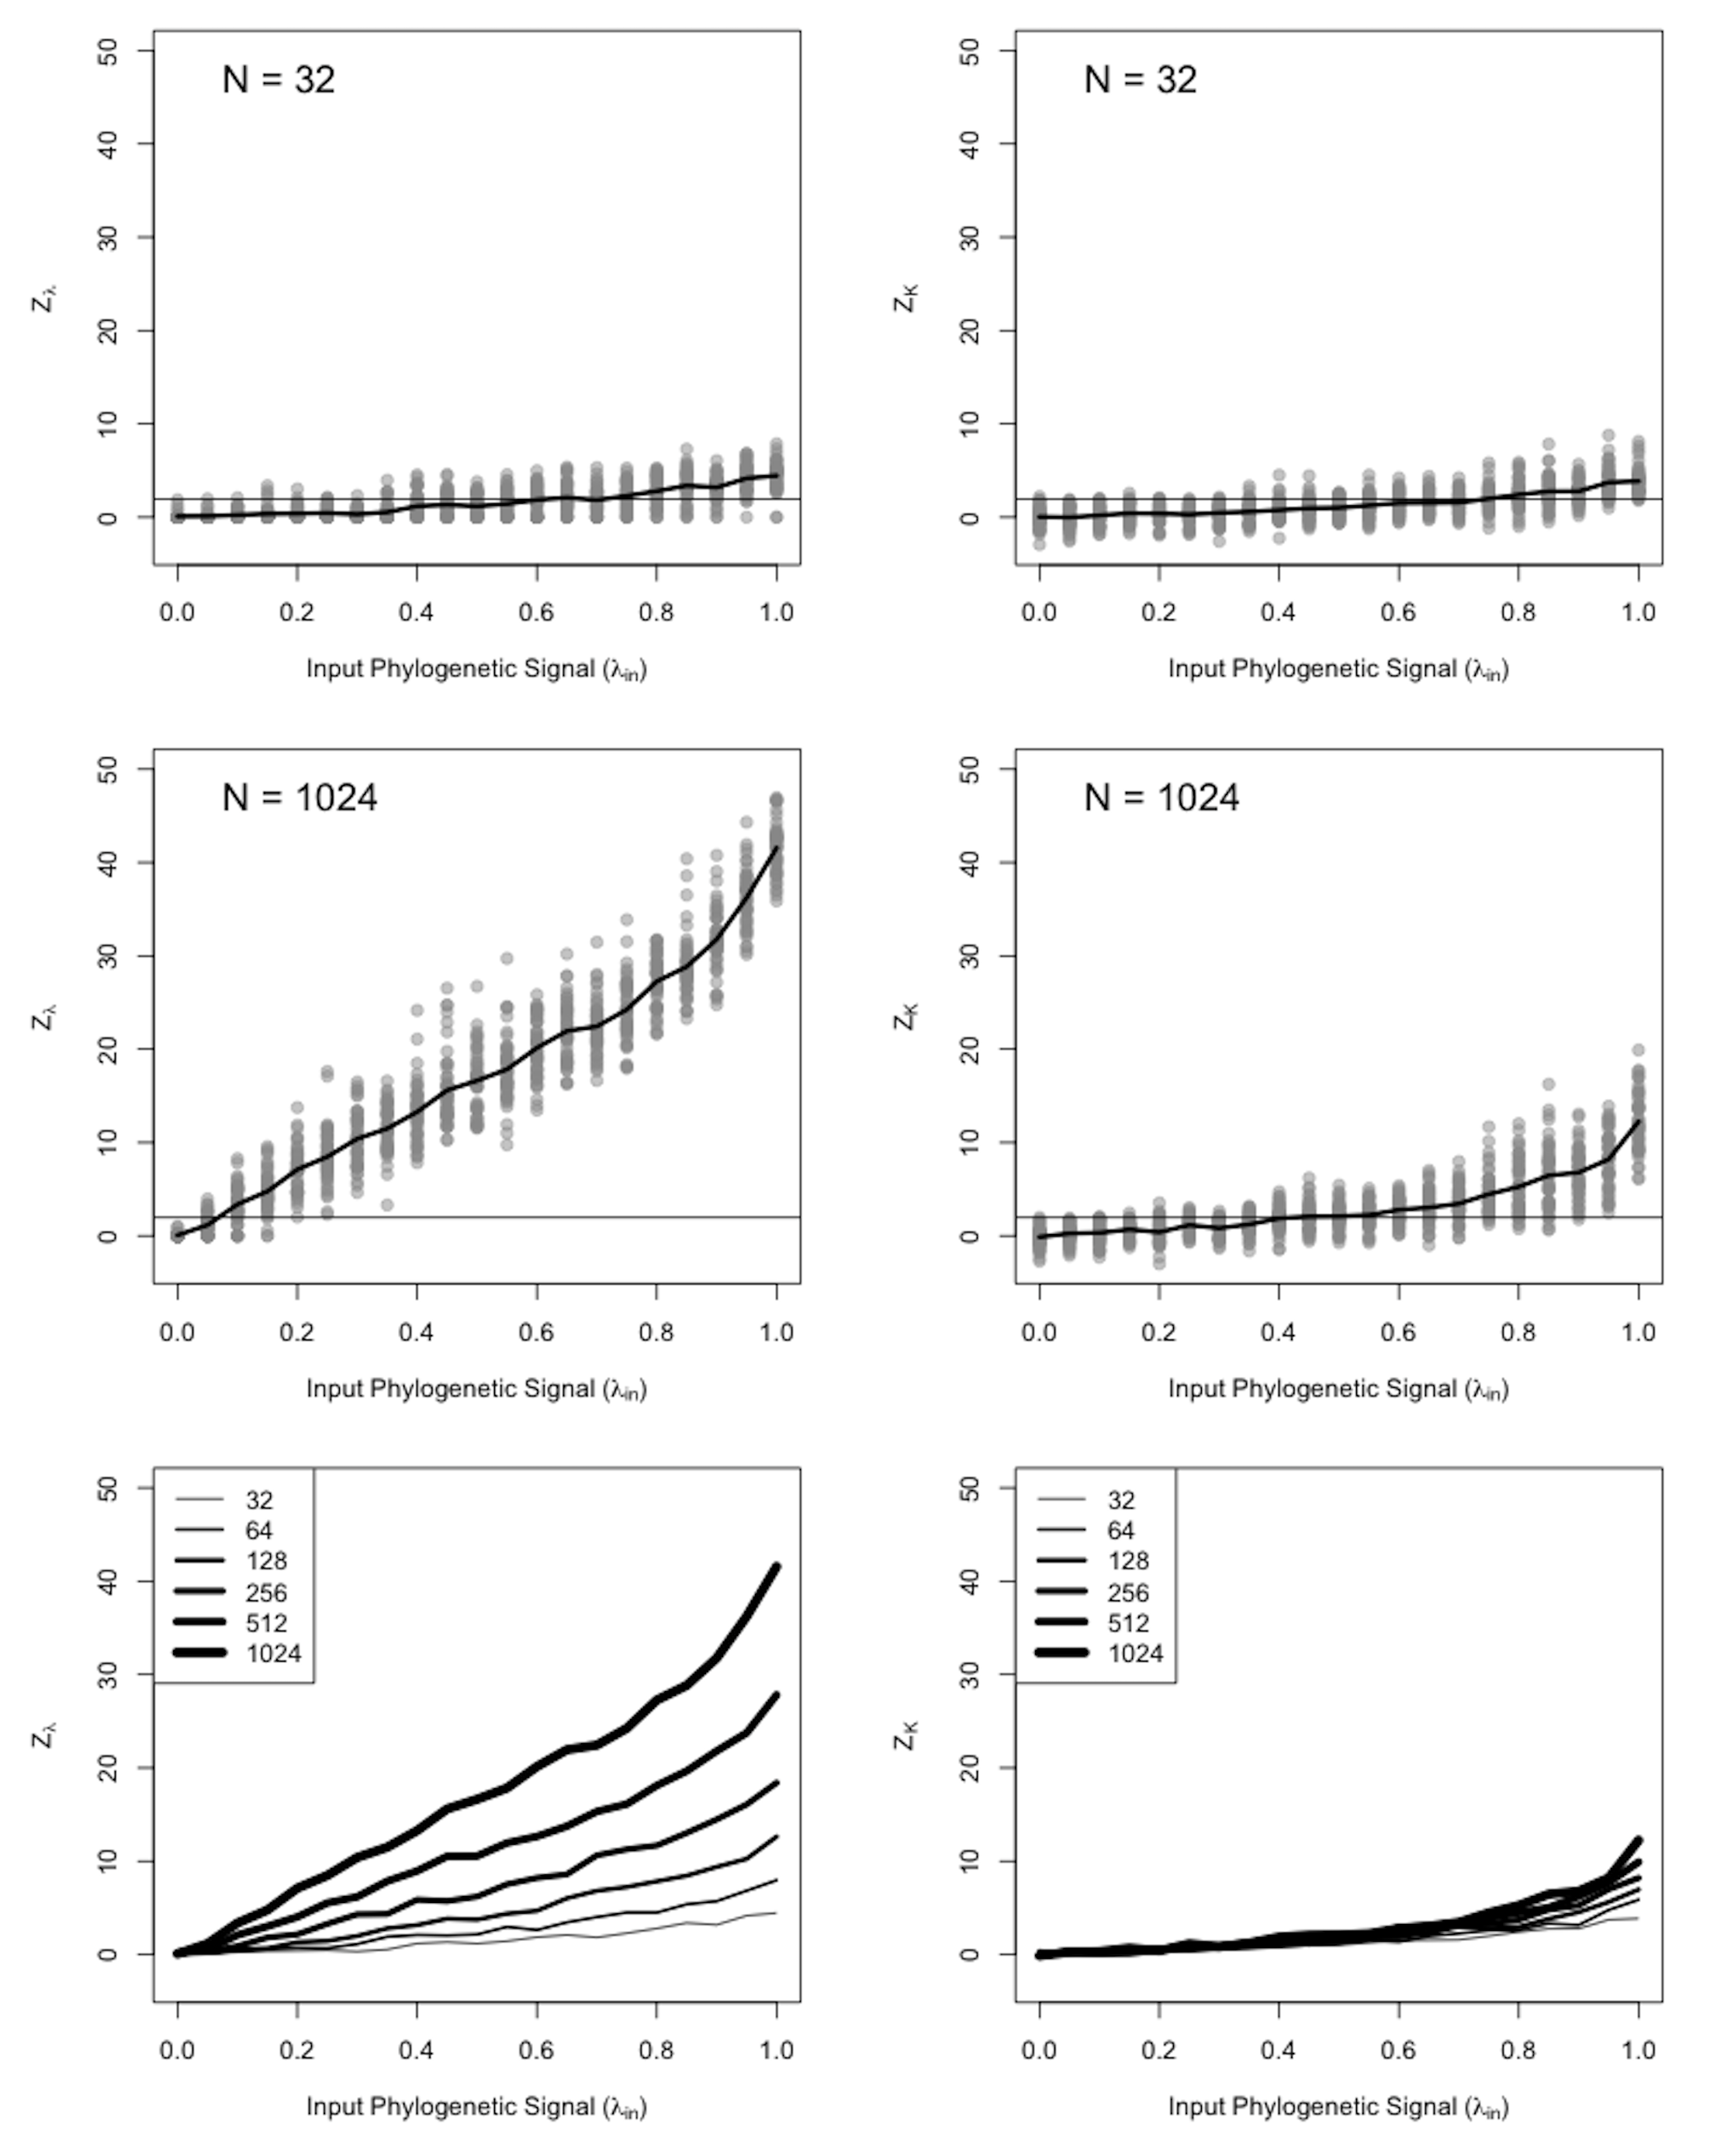
\includegraphics[width=0.95\linewidth]{fig.S10}

\textbf{Figure S10}. Response of effect sizes \(Z_{\lambda}\) and
\(Z_K\) to increasing strength of Brownian motion for pure-birth trees
containing polytomies.

\newpage

\hypertarget{simulations-of-phylogenetic-regression-and-anova}{%
\subsection{Simulations of Phylogenetic Regression and
ANOVA}\label{simulations-of-phylogenetic-regression-and-anova}}

We also investigated the effect of incorporating \(\lambda\) in PGLS
analyses (phylogenetic regression and ANOVA). Here, patterns for
\(\hat\lambda\), \emph{K}, \(Z_\lambda\) and \(Z_K\) were virtually
identical to those found previously. In essence, \(\hat\lambda\) was not
suitable as a test statistic representing phylogenetic signal due to all
properties previously shown (Figs. S11 \& S12), \emph{K} was more
appropriate, but associated non-linearly with signal strength (Figs. S13
\& 14), while \(Z_K\) was found to be a superior effect size as compared
with \(Z_\lambda\) (Figs S15 \& S16). \hfill\break

With respect to model performance, input parameters (\(\beta\)) were
well estimated in phylogenetic regression and ANOVA when \(\lambda\) was
incorporated (Figs S17 \& S18), implying that \(\lambda\) may be used as
a tuning parameter for these models. Additionally, type I error and
statistical power were unaffected by the inclusion of \(\lambda\) (Figs
S19 \& S20), though power was reduced at smaller sample sizes in
phylogenetic ANOVA, mirroring prior findings of (2). These results
generally confirmed earlier findings of (3) for phylogenetic regression,
and extend them to the case of phylogenetic ANOVA.

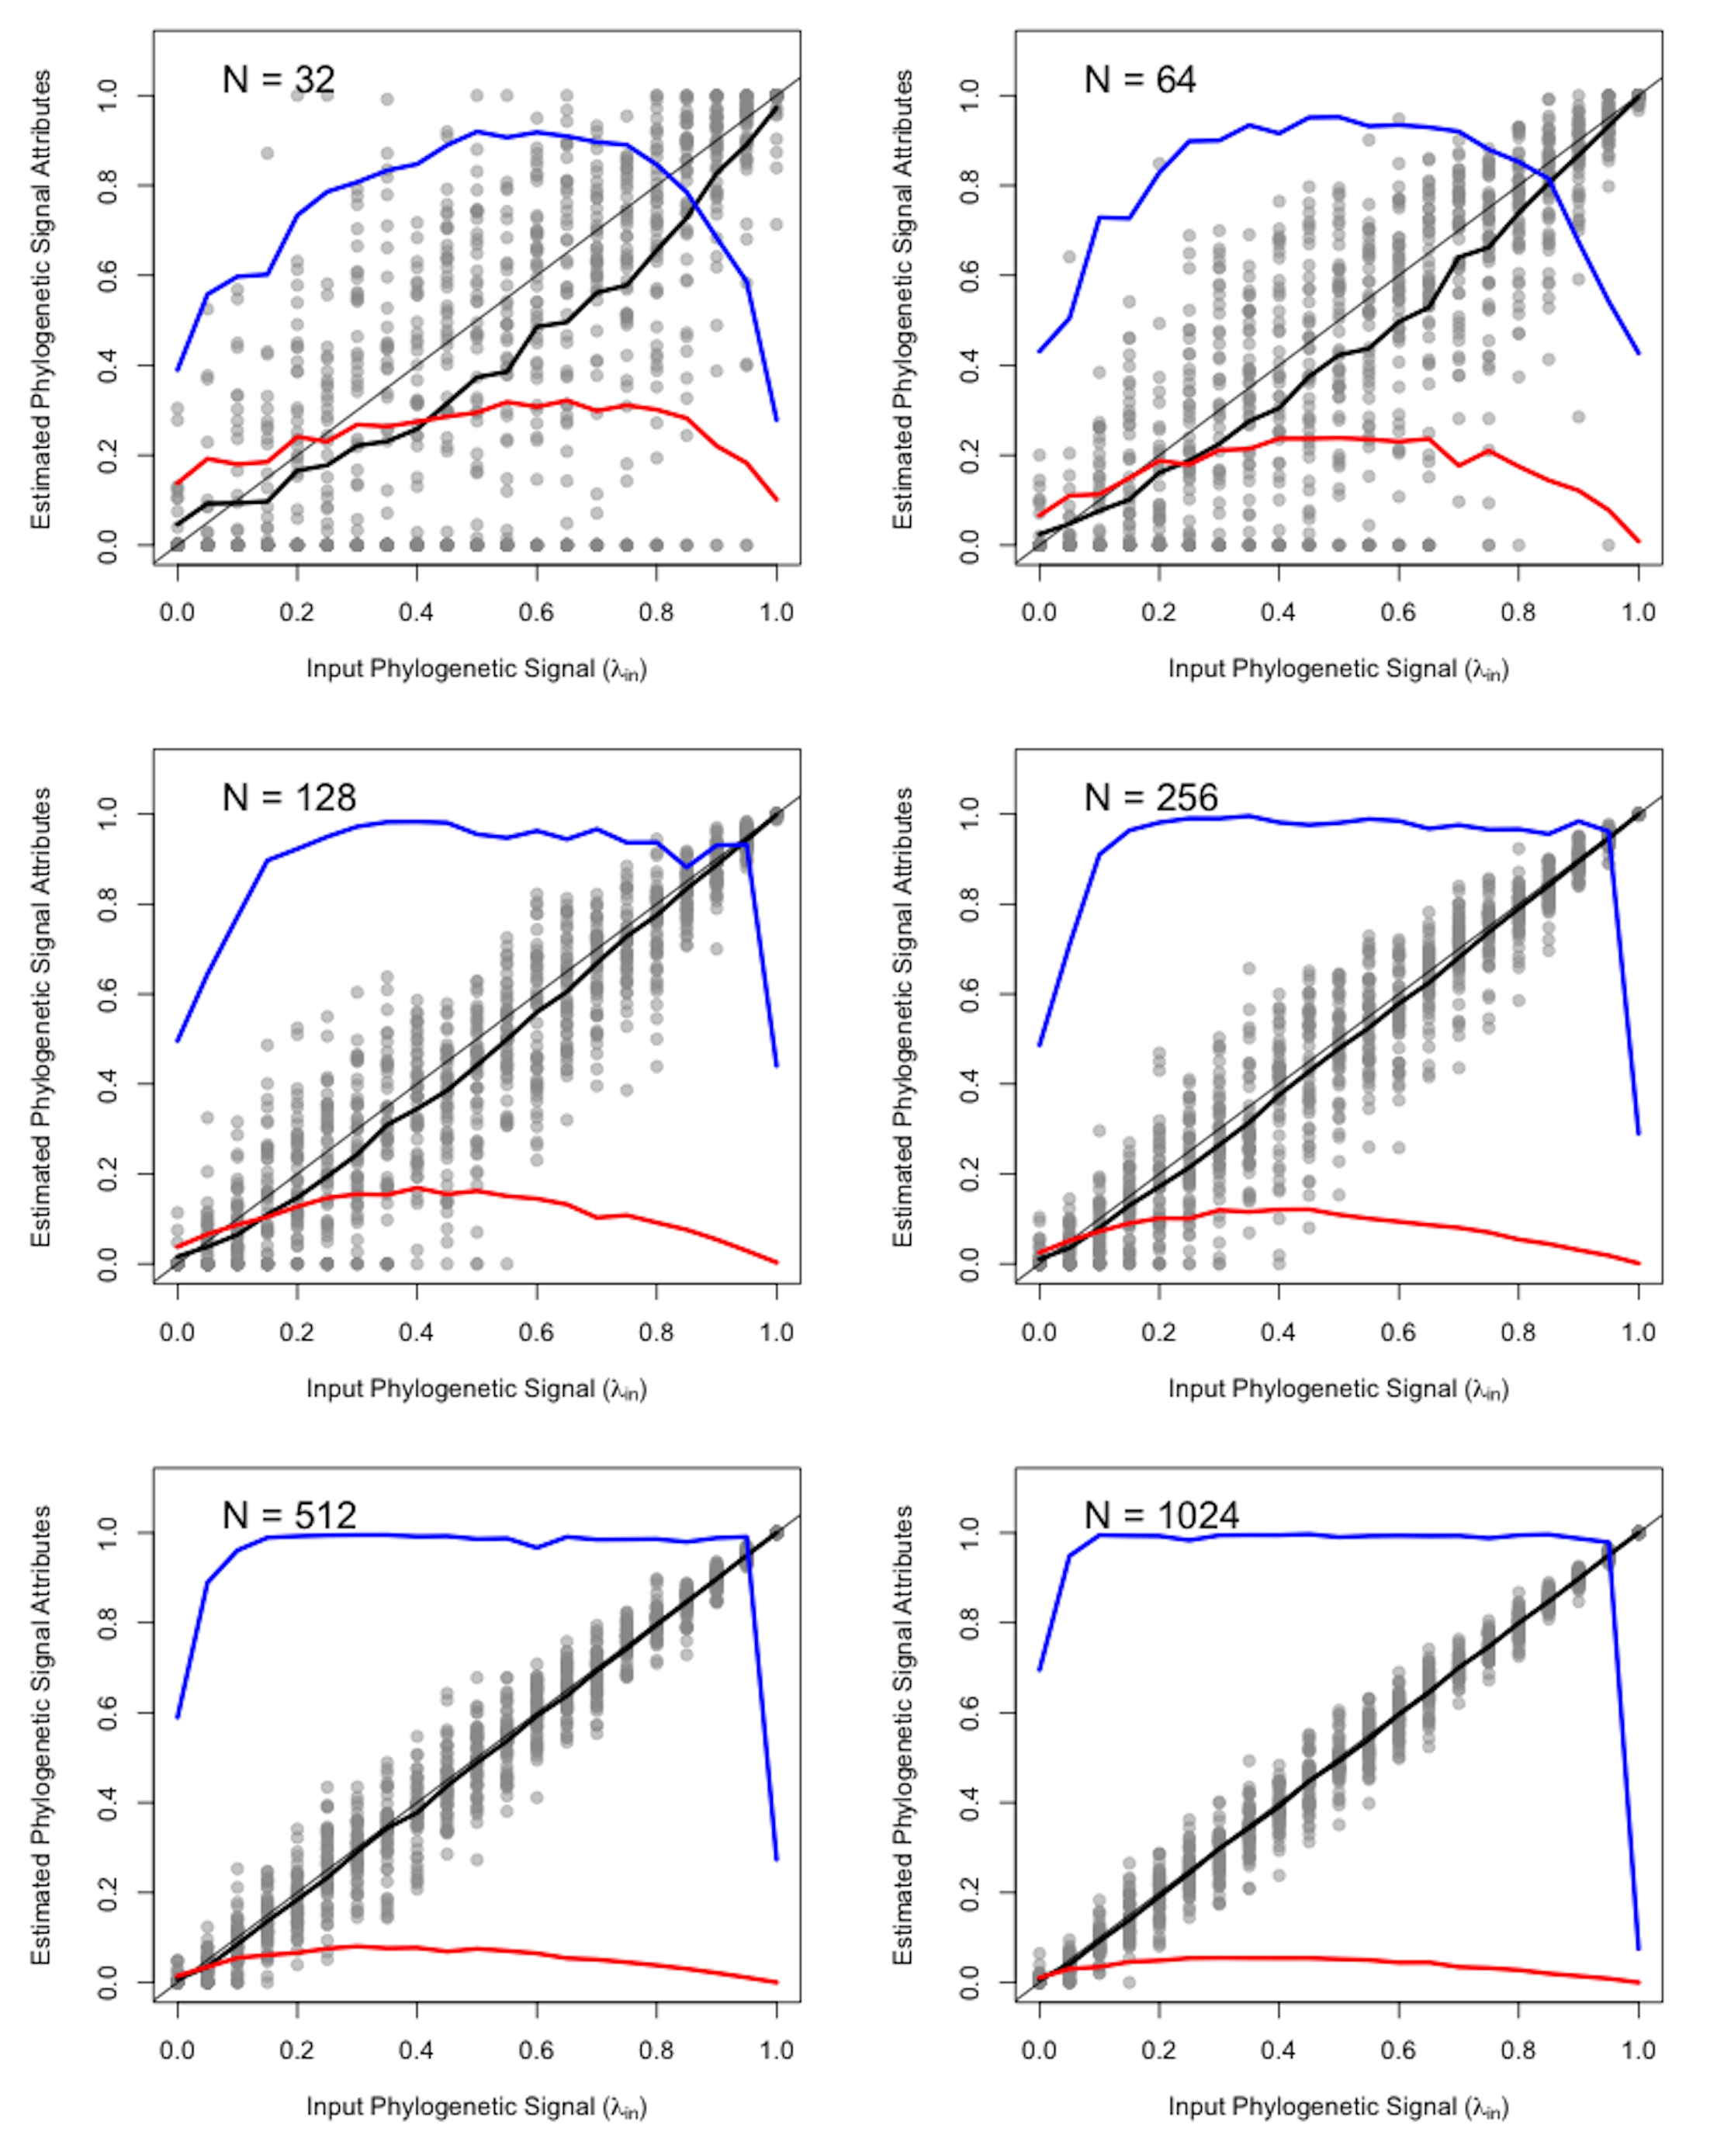
\includegraphics[width=0.95\linewidth]{fig.S11}

\textbf{Figure S11}. Response of Pagel's \(\lambda\) to increasing
strength of Brownian motion in phylogenetic regression (incorporating
\(\lambda\)). Gray line signifies the 1:1 line where the input value
matches the estimate. At each input level, the dark black line
represents the empirically derived expected value (mean) of
\(\hat\lambda\), the red line is the standard deviation of
\(\hat\lambda\), and the blue line is Shapiro Wilks statistic of
\(\hat\lambda\) (\(W=1.0\) signifies normality, \(W< 1.0\) represent
skewed distributions).

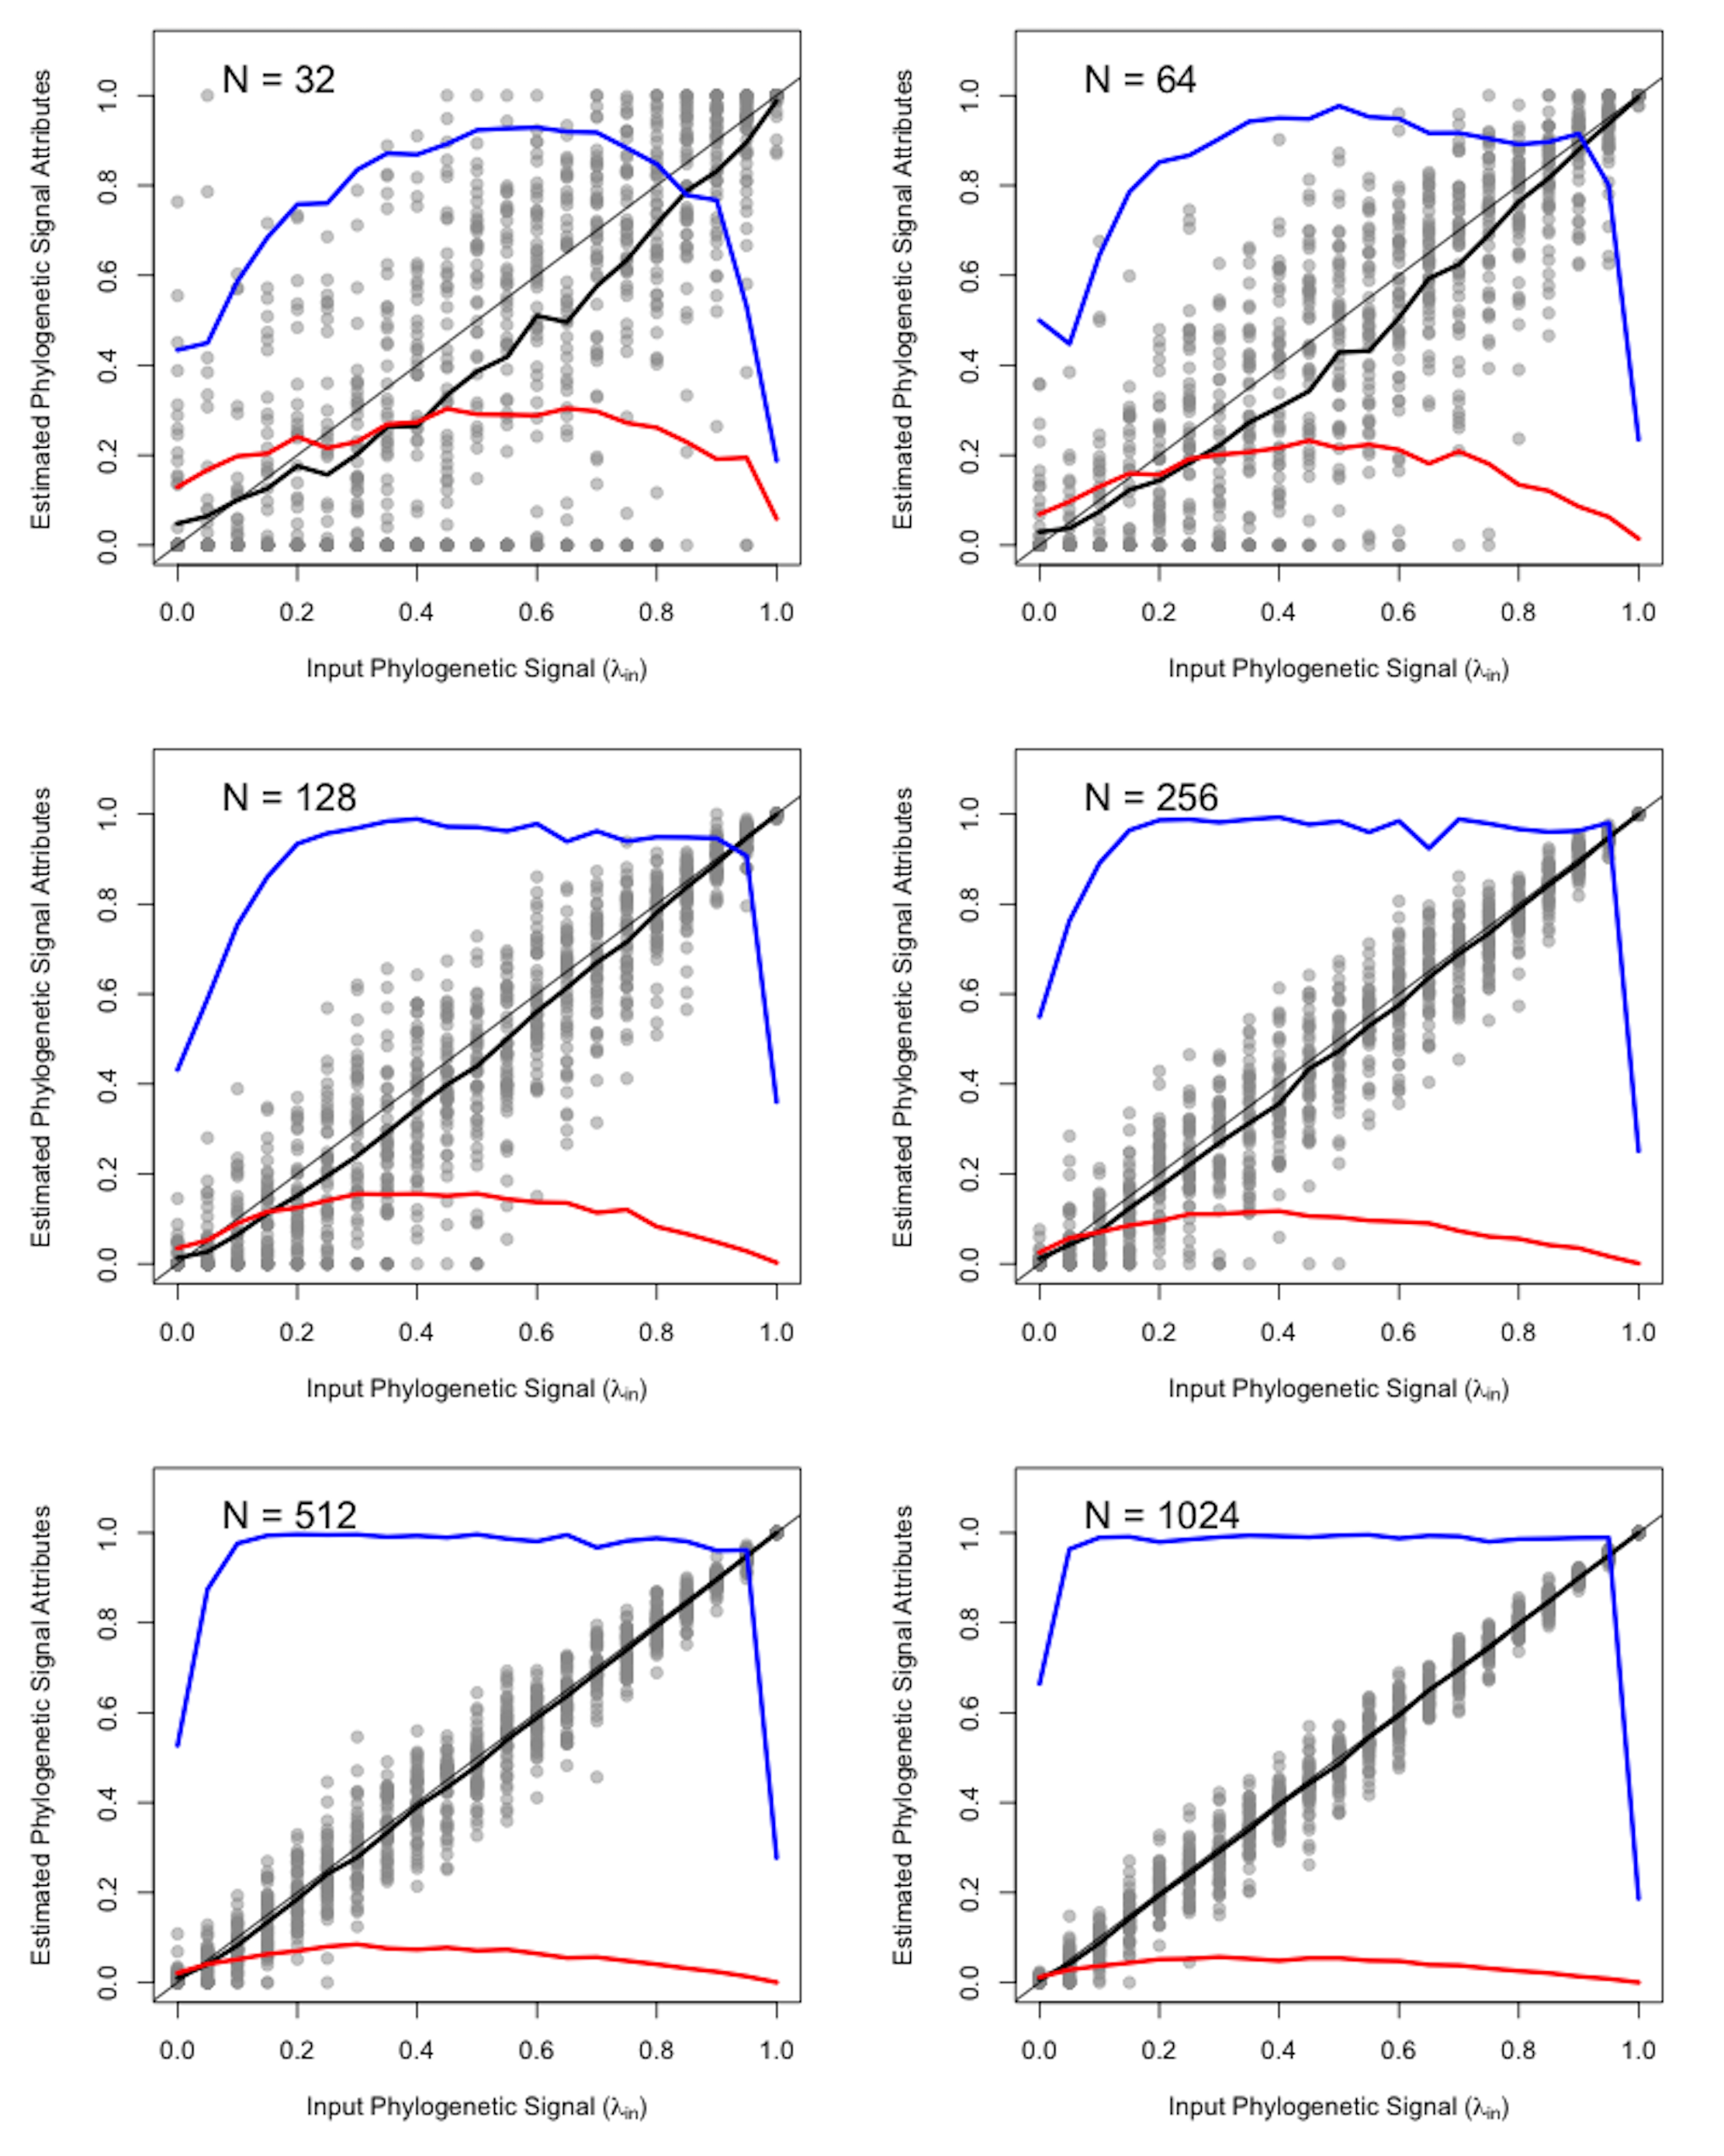
\includegraphics[width=0.95\linewidth]{fig.S12}

\textbf{Figure S12}. Response of Pagel's \(\lambda\) to increasing
strength of Brownian motion in phylogenetic ANOVA (incorporating
\(\lambda\)). Gray line signifies the 1:1 line where the input value
matches the estimate. At each input level, the dark black line
represents the empirically derived expected value (mean) of
\(\hat\lambda\), the red line is the standard deviation of
\(\hat\lambda\), and the blue line is Shapiro Wilks statistic of
\(\hat\lambda\) (\(W=1.0\) signifies normality, \(W< 1.0\) represent
skewed distributions).

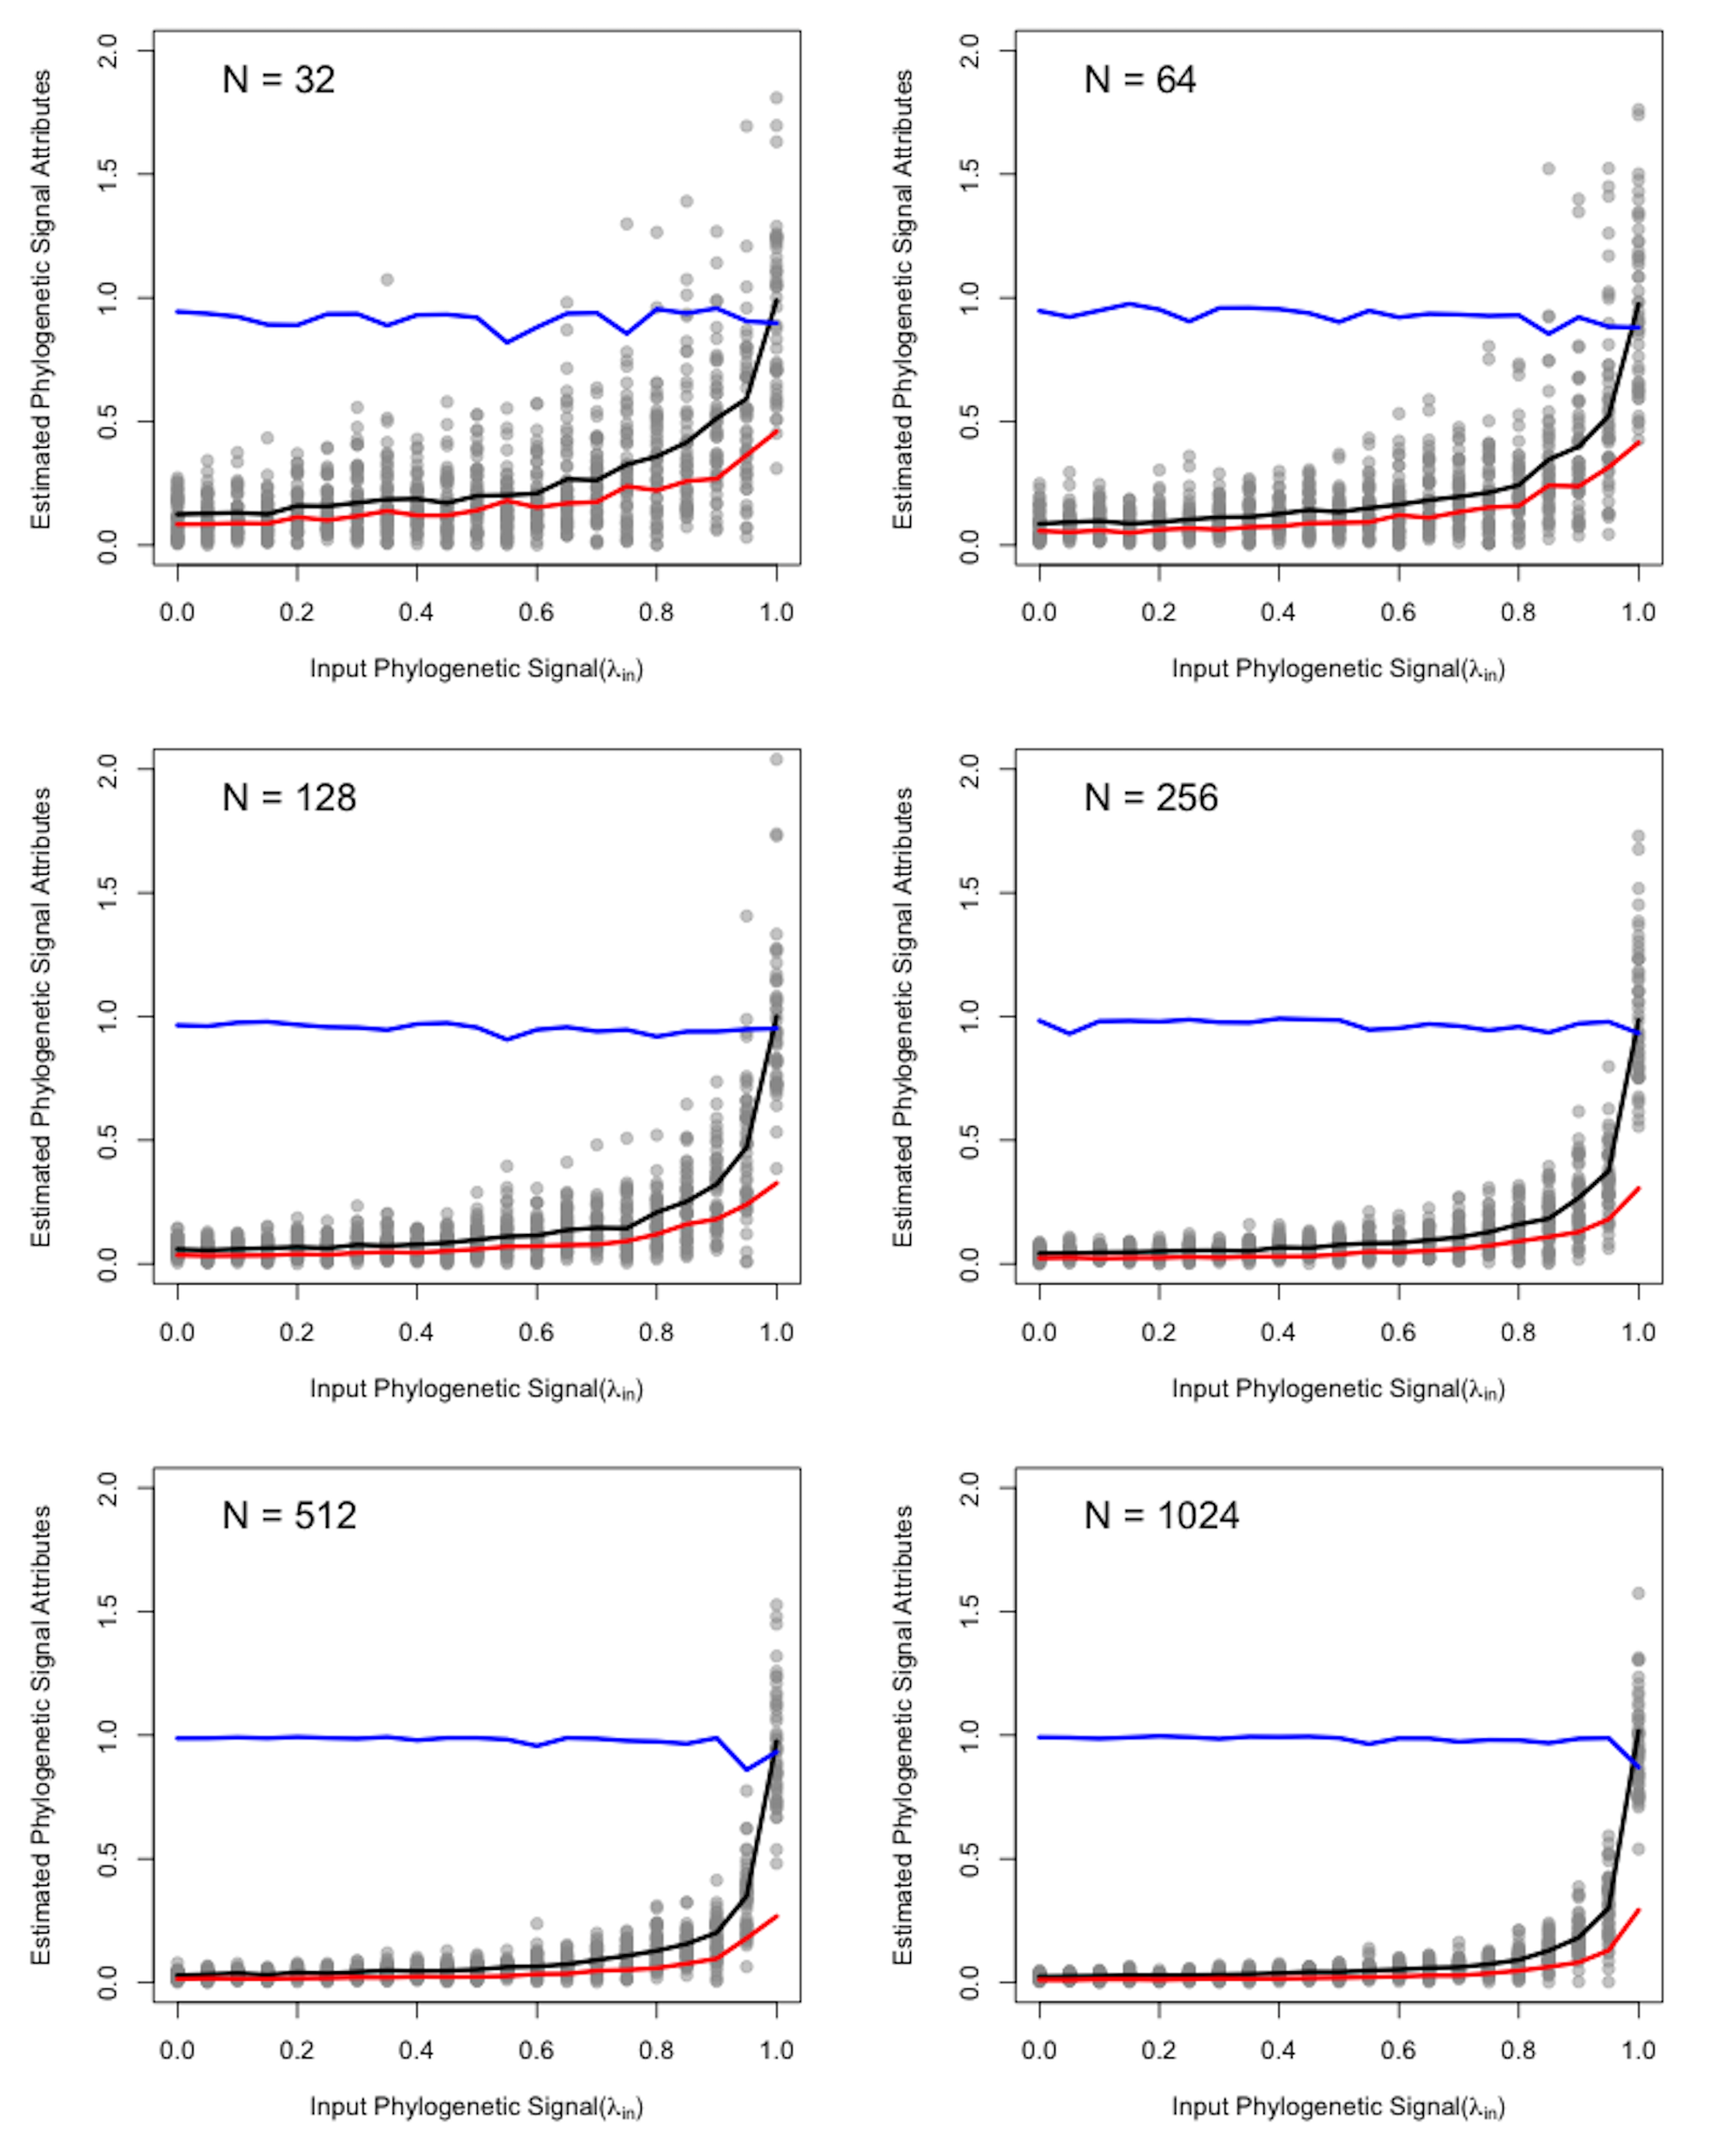
\includegraphics[width=0.95\linewidth]{fig.S13}

\textbf{Figure S13}. Response of Blomberg's \textit{K} to increasing
strength of Brownian motion in phylogenetic regression (incorporating
\(\lambda\)). At each input level, the dark black line represents the
empirically derived expected value (mean) of \textit{K}, the red line is
the standard deviation of \textit{K}, and the blue line is Shapiro Wilks
statistic of \textit{K} (\(W=1.0\) signifies normality, \(W< 1.0\)
represent skewed distributions).

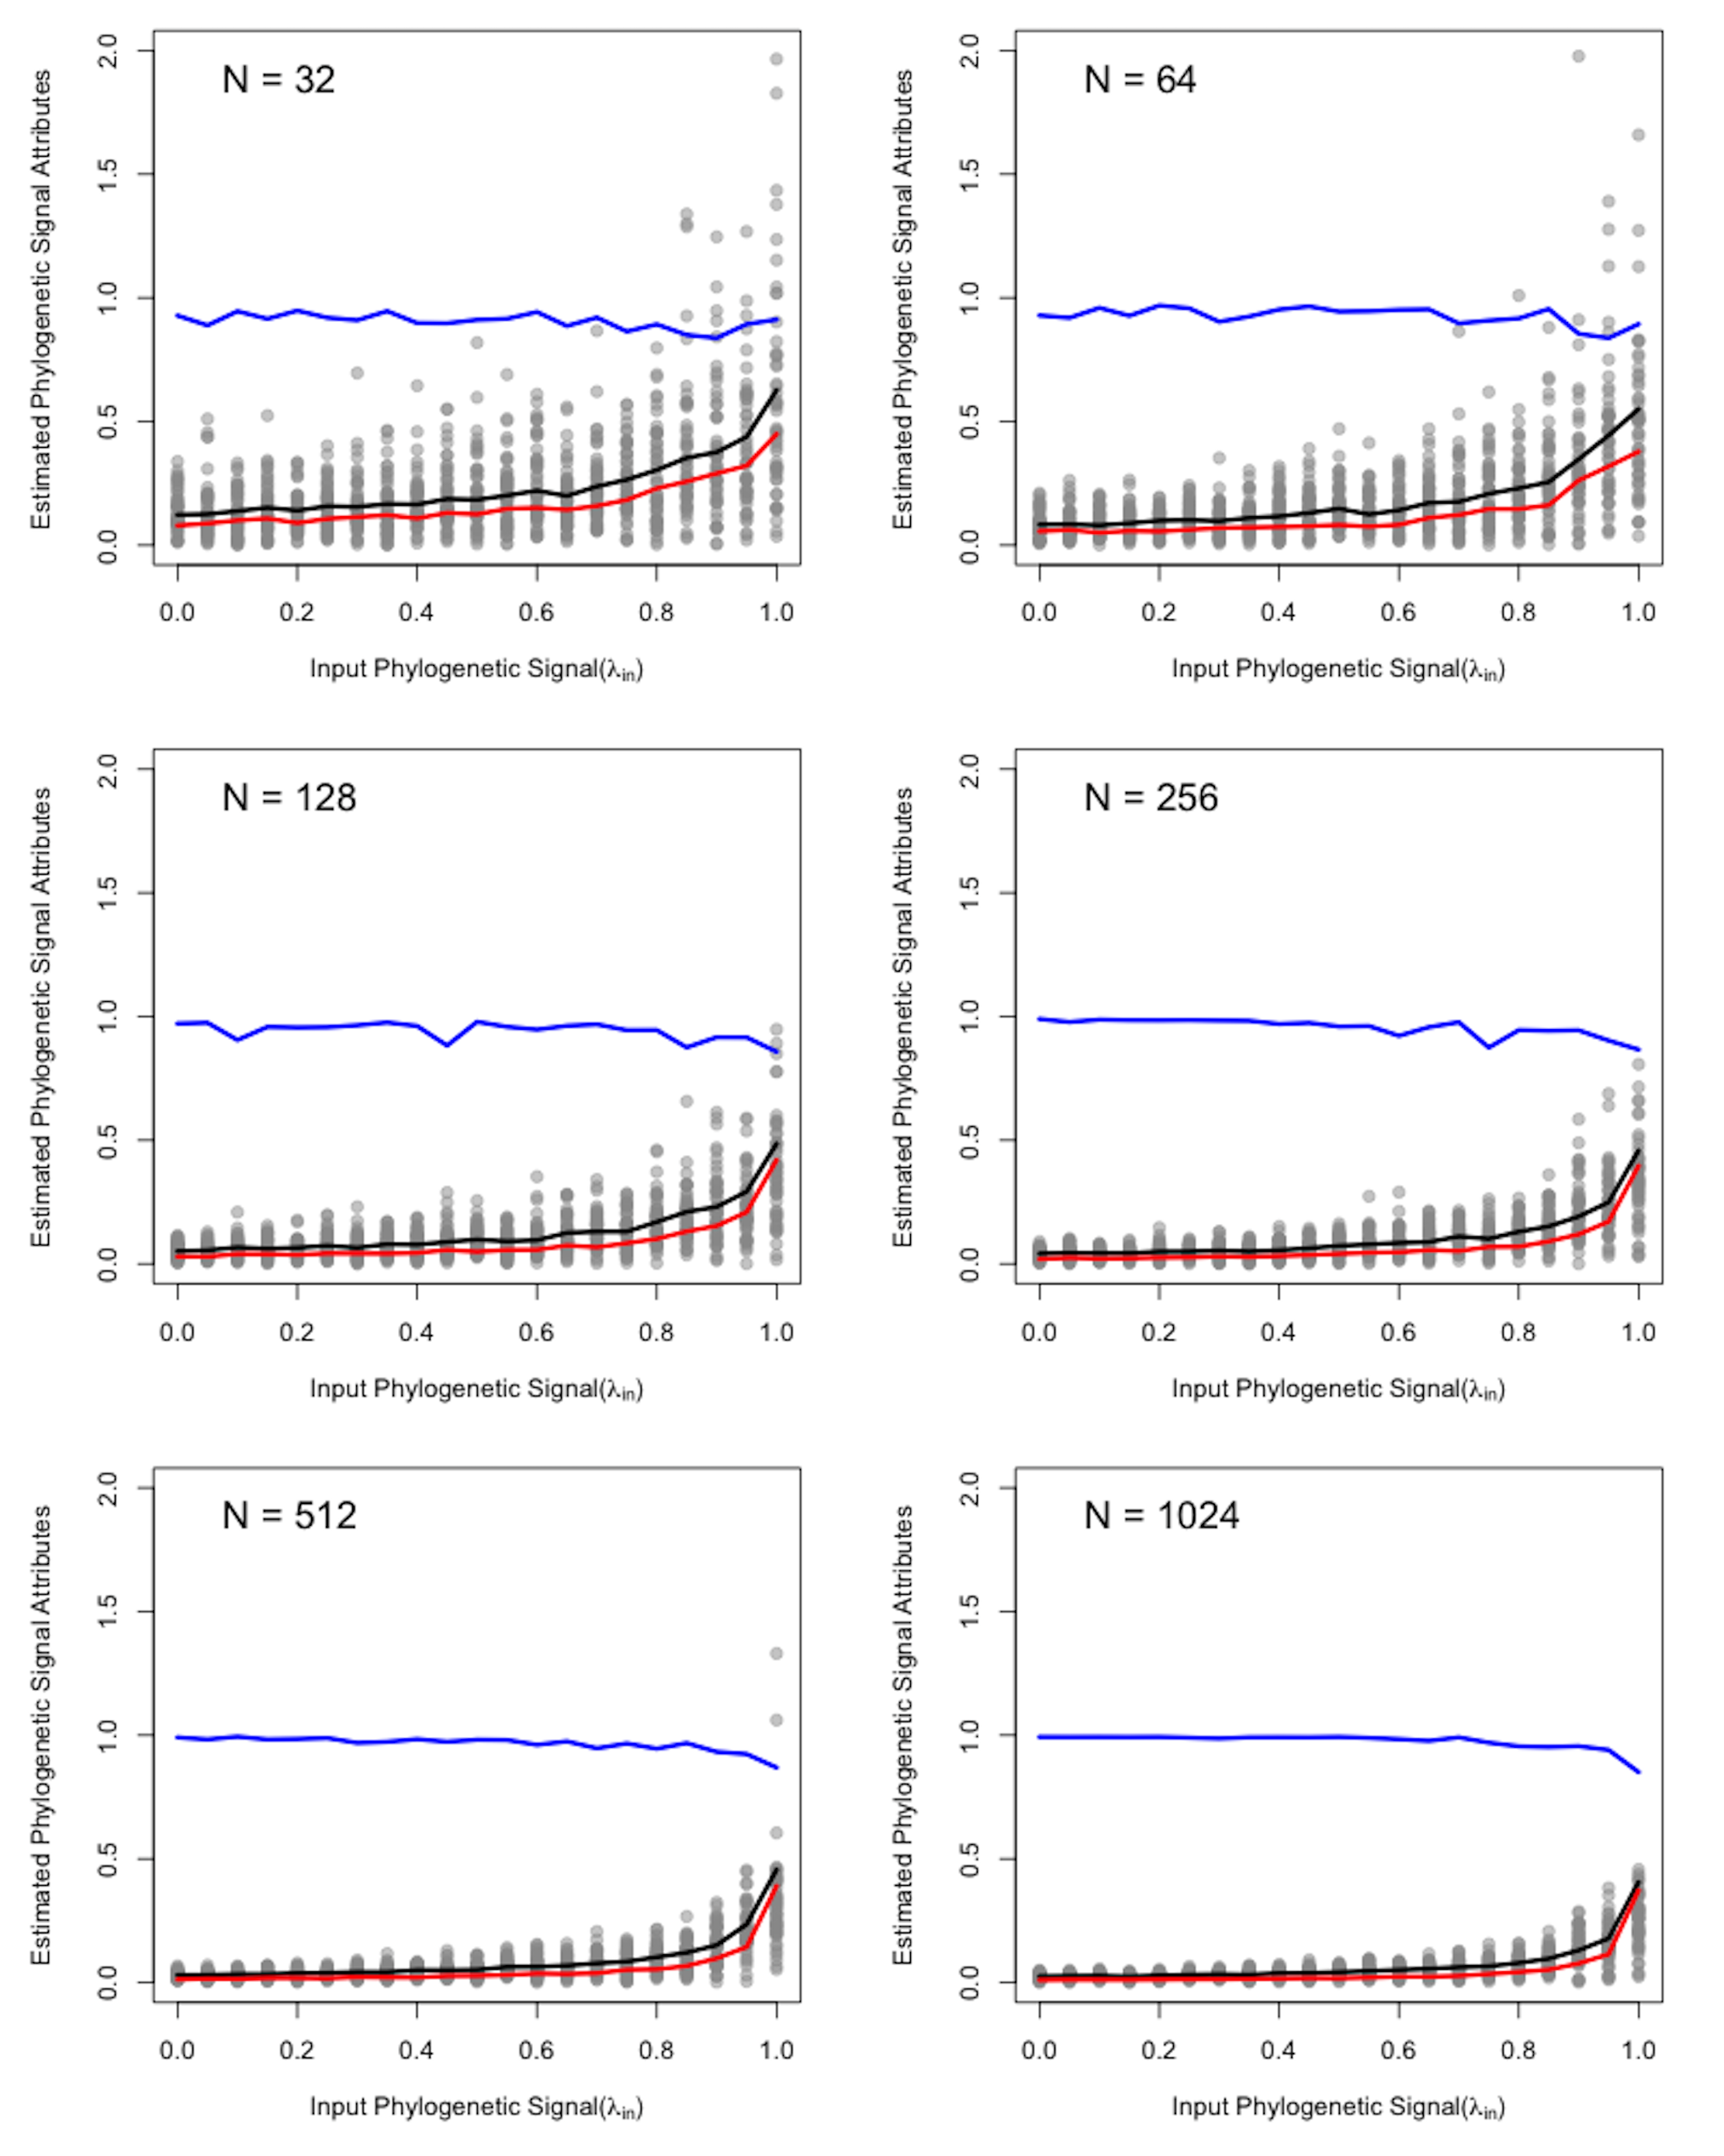
\includegraphics[width=0.95\linewidth]{fig.S14}

\textbf{Figure S14}. Response of Blomberg's \textit{K} to increasing
strength of Brownian motion in phylogenetic ANOVA (incorporating
\(\lambda\)). At each input level, the dark black line represents the
empirically derived expected value (mean) of \textit{K}, the red line is
the standard deviation of \textit{K}, and the blue line is Shapiro Wilks
statistic of \textit{K} (\(W=1.0\) signifies normality, \(W< 1.0\)
represent skewed distributions).

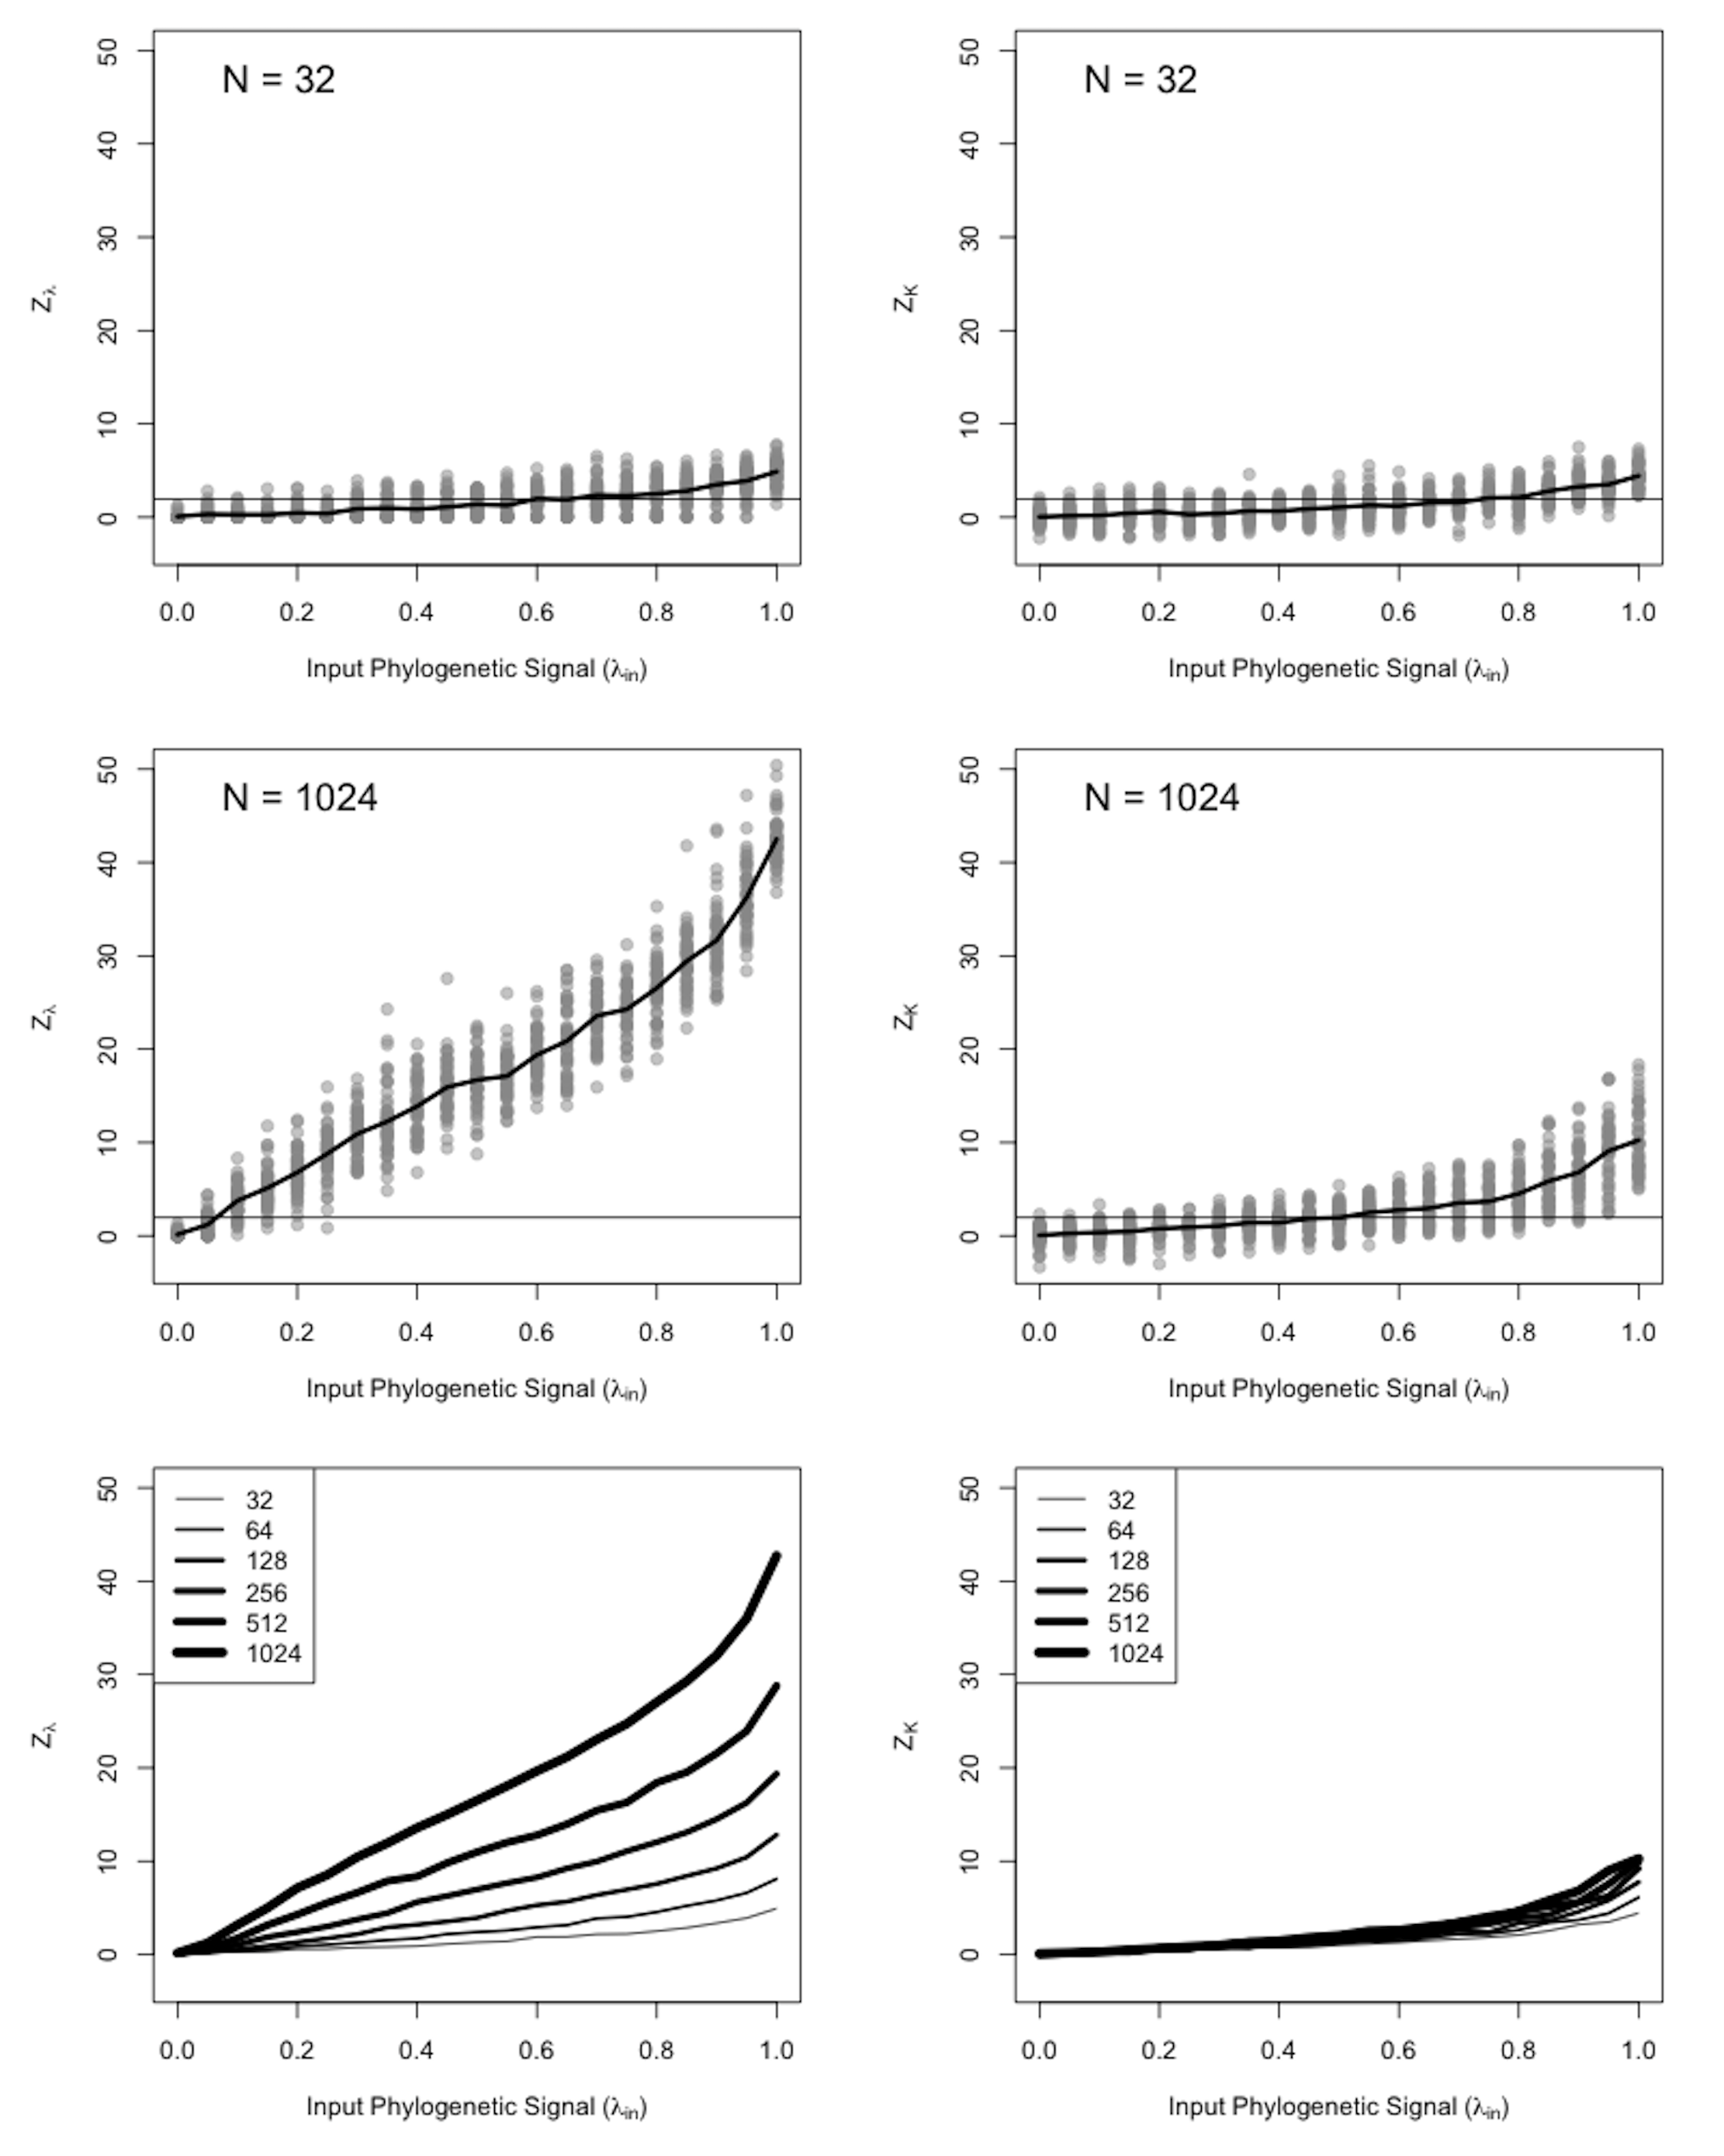
\includegraphics[width=0.95\linewidth]{fig.S15}

\textbf{Figure S15}. Response of effect sizes \(Z_{\lambda}\) and
\(Z_K\) to increasing strength of Brownian motion in phylogenetic
regression (incorporating \(\lambda\)).

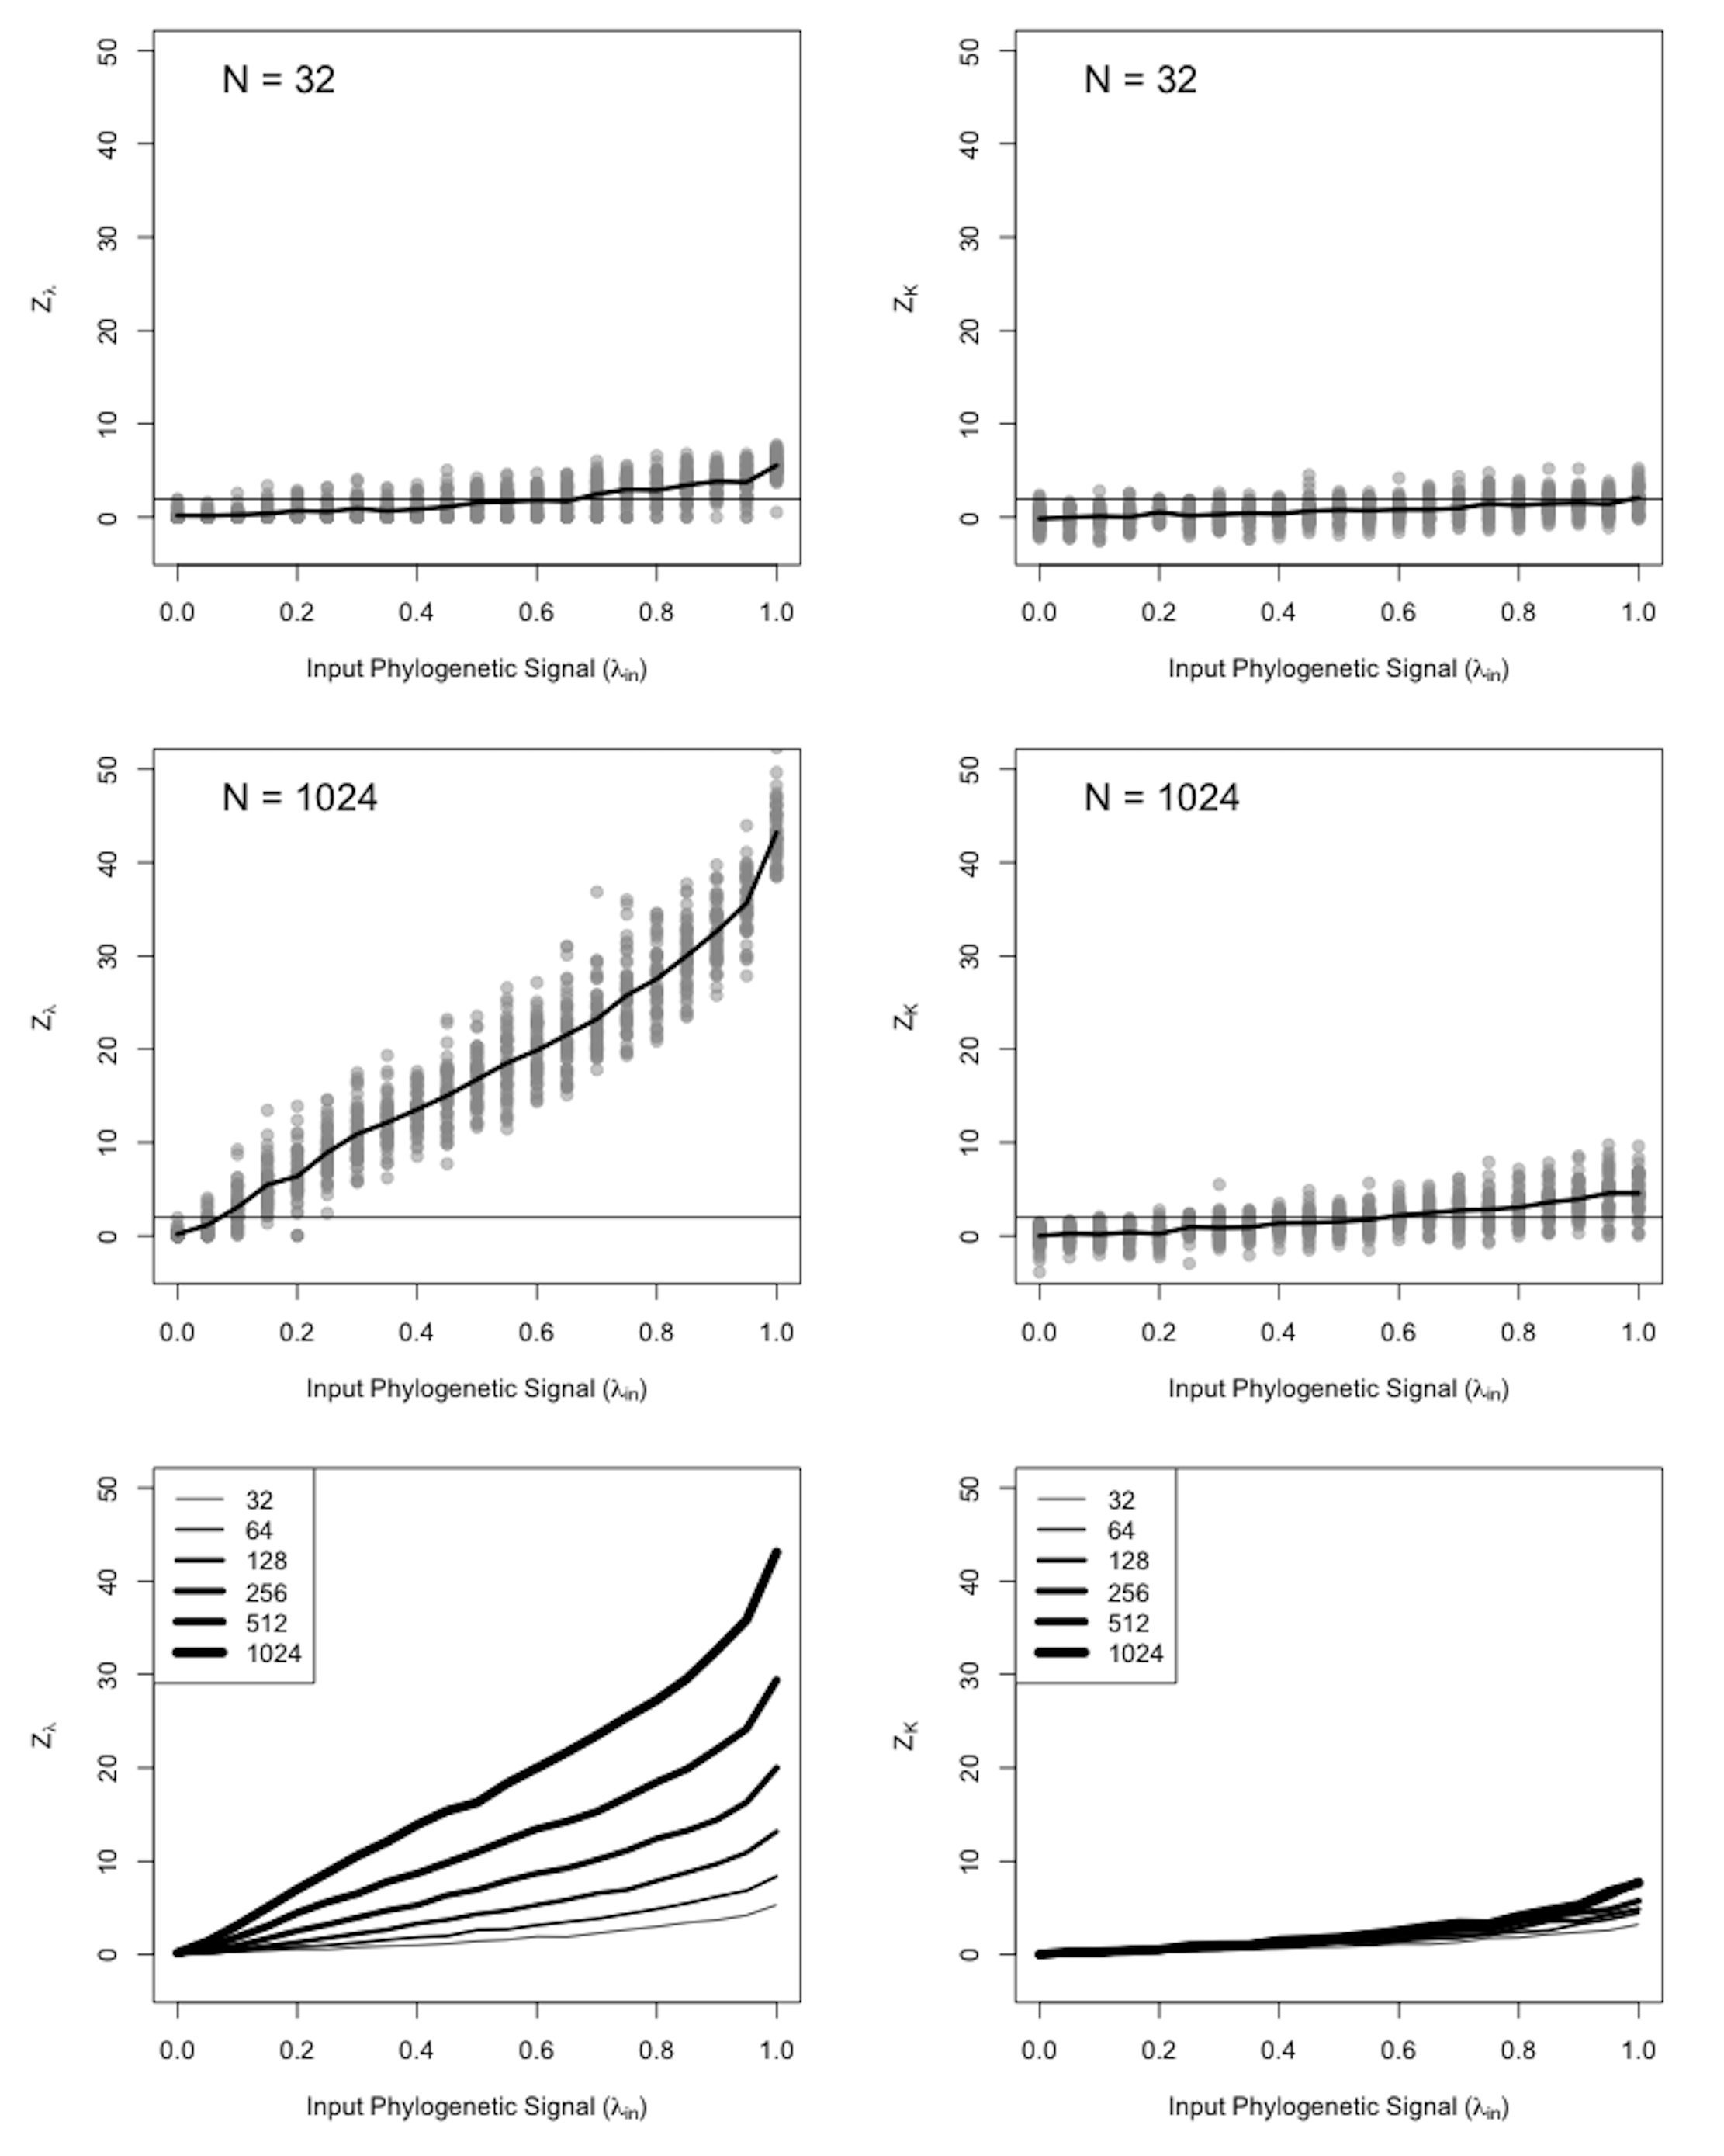
\includegraphics[width=0.95\linewidth]{fig.S16}

\textbf{Figure S16}. Response of effect sizes \(Z_{\lambda}\) and
\(Z_K\) to increasing strength of Brownian motion in phylogenetic ANOVA
(incorporating \(\lambda\)).

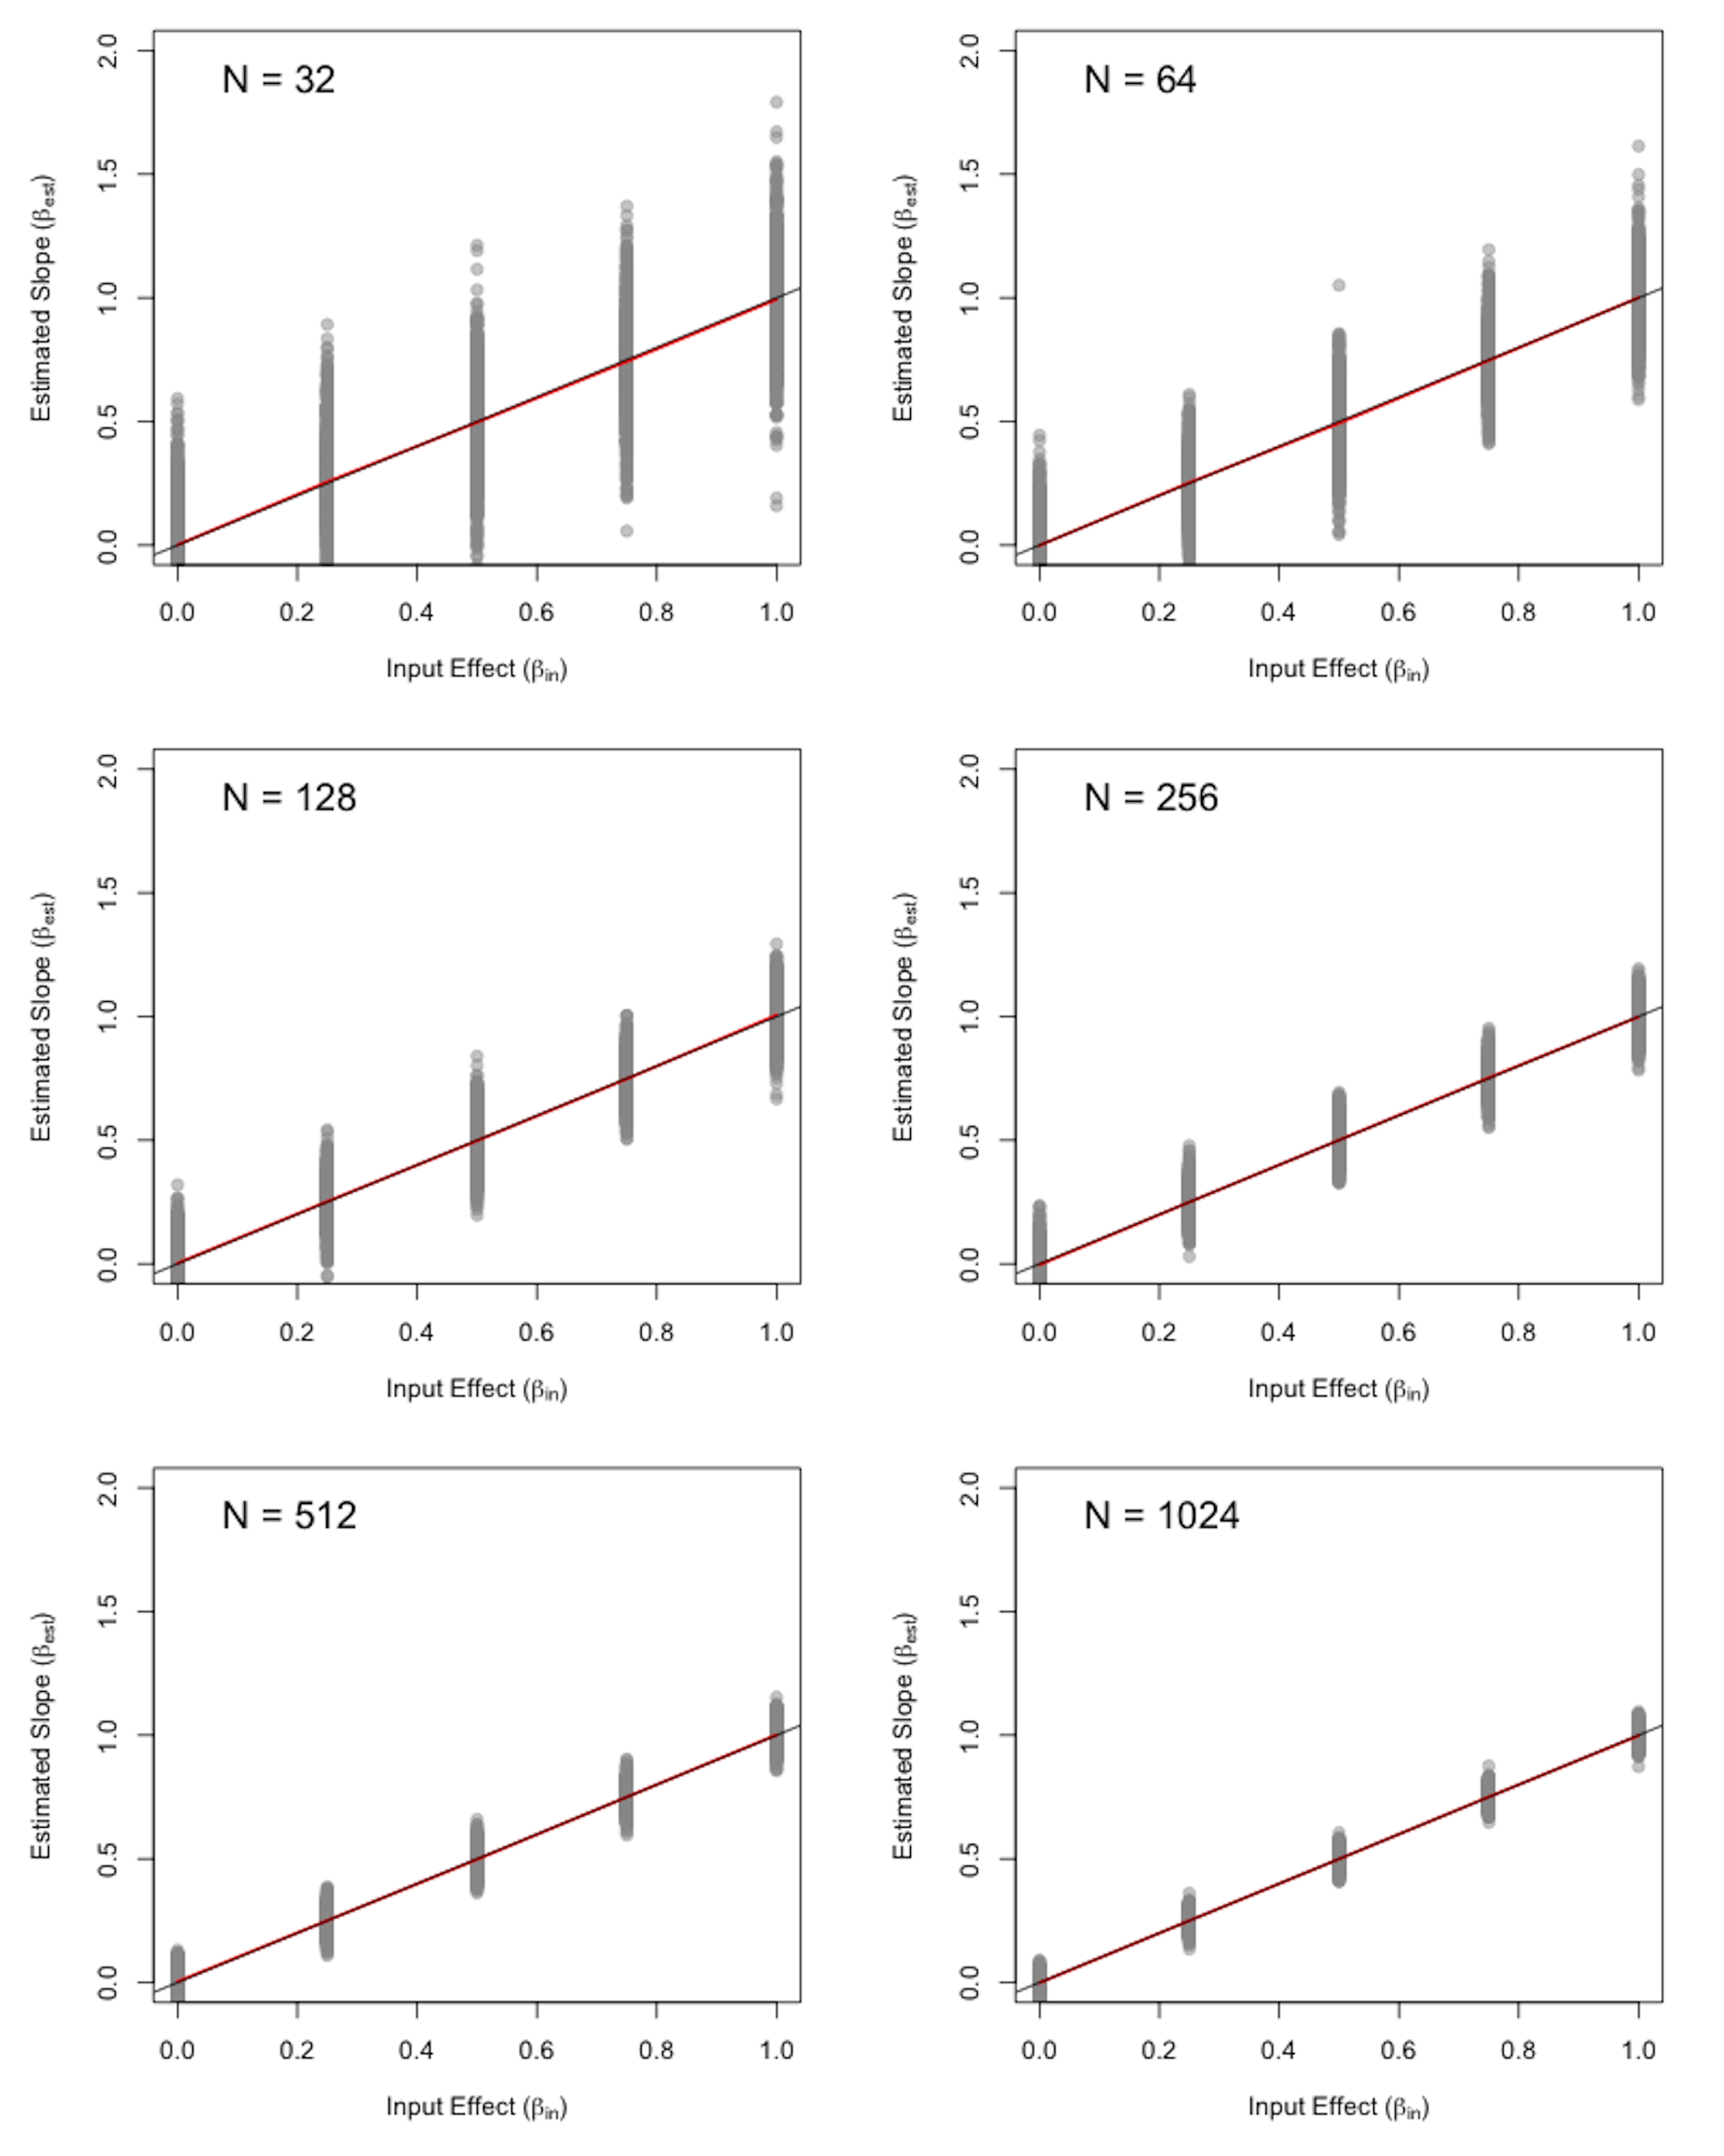
\includegraphics[width=0.95\linewidth]{fig.S17}

\textbf{Figure S17}. Parameter estimates from phylogenetic regression
(incorporating \(\lambda\)). The red line represents the estimated
slope, which almost completely overlaps the gray 1:1 line.

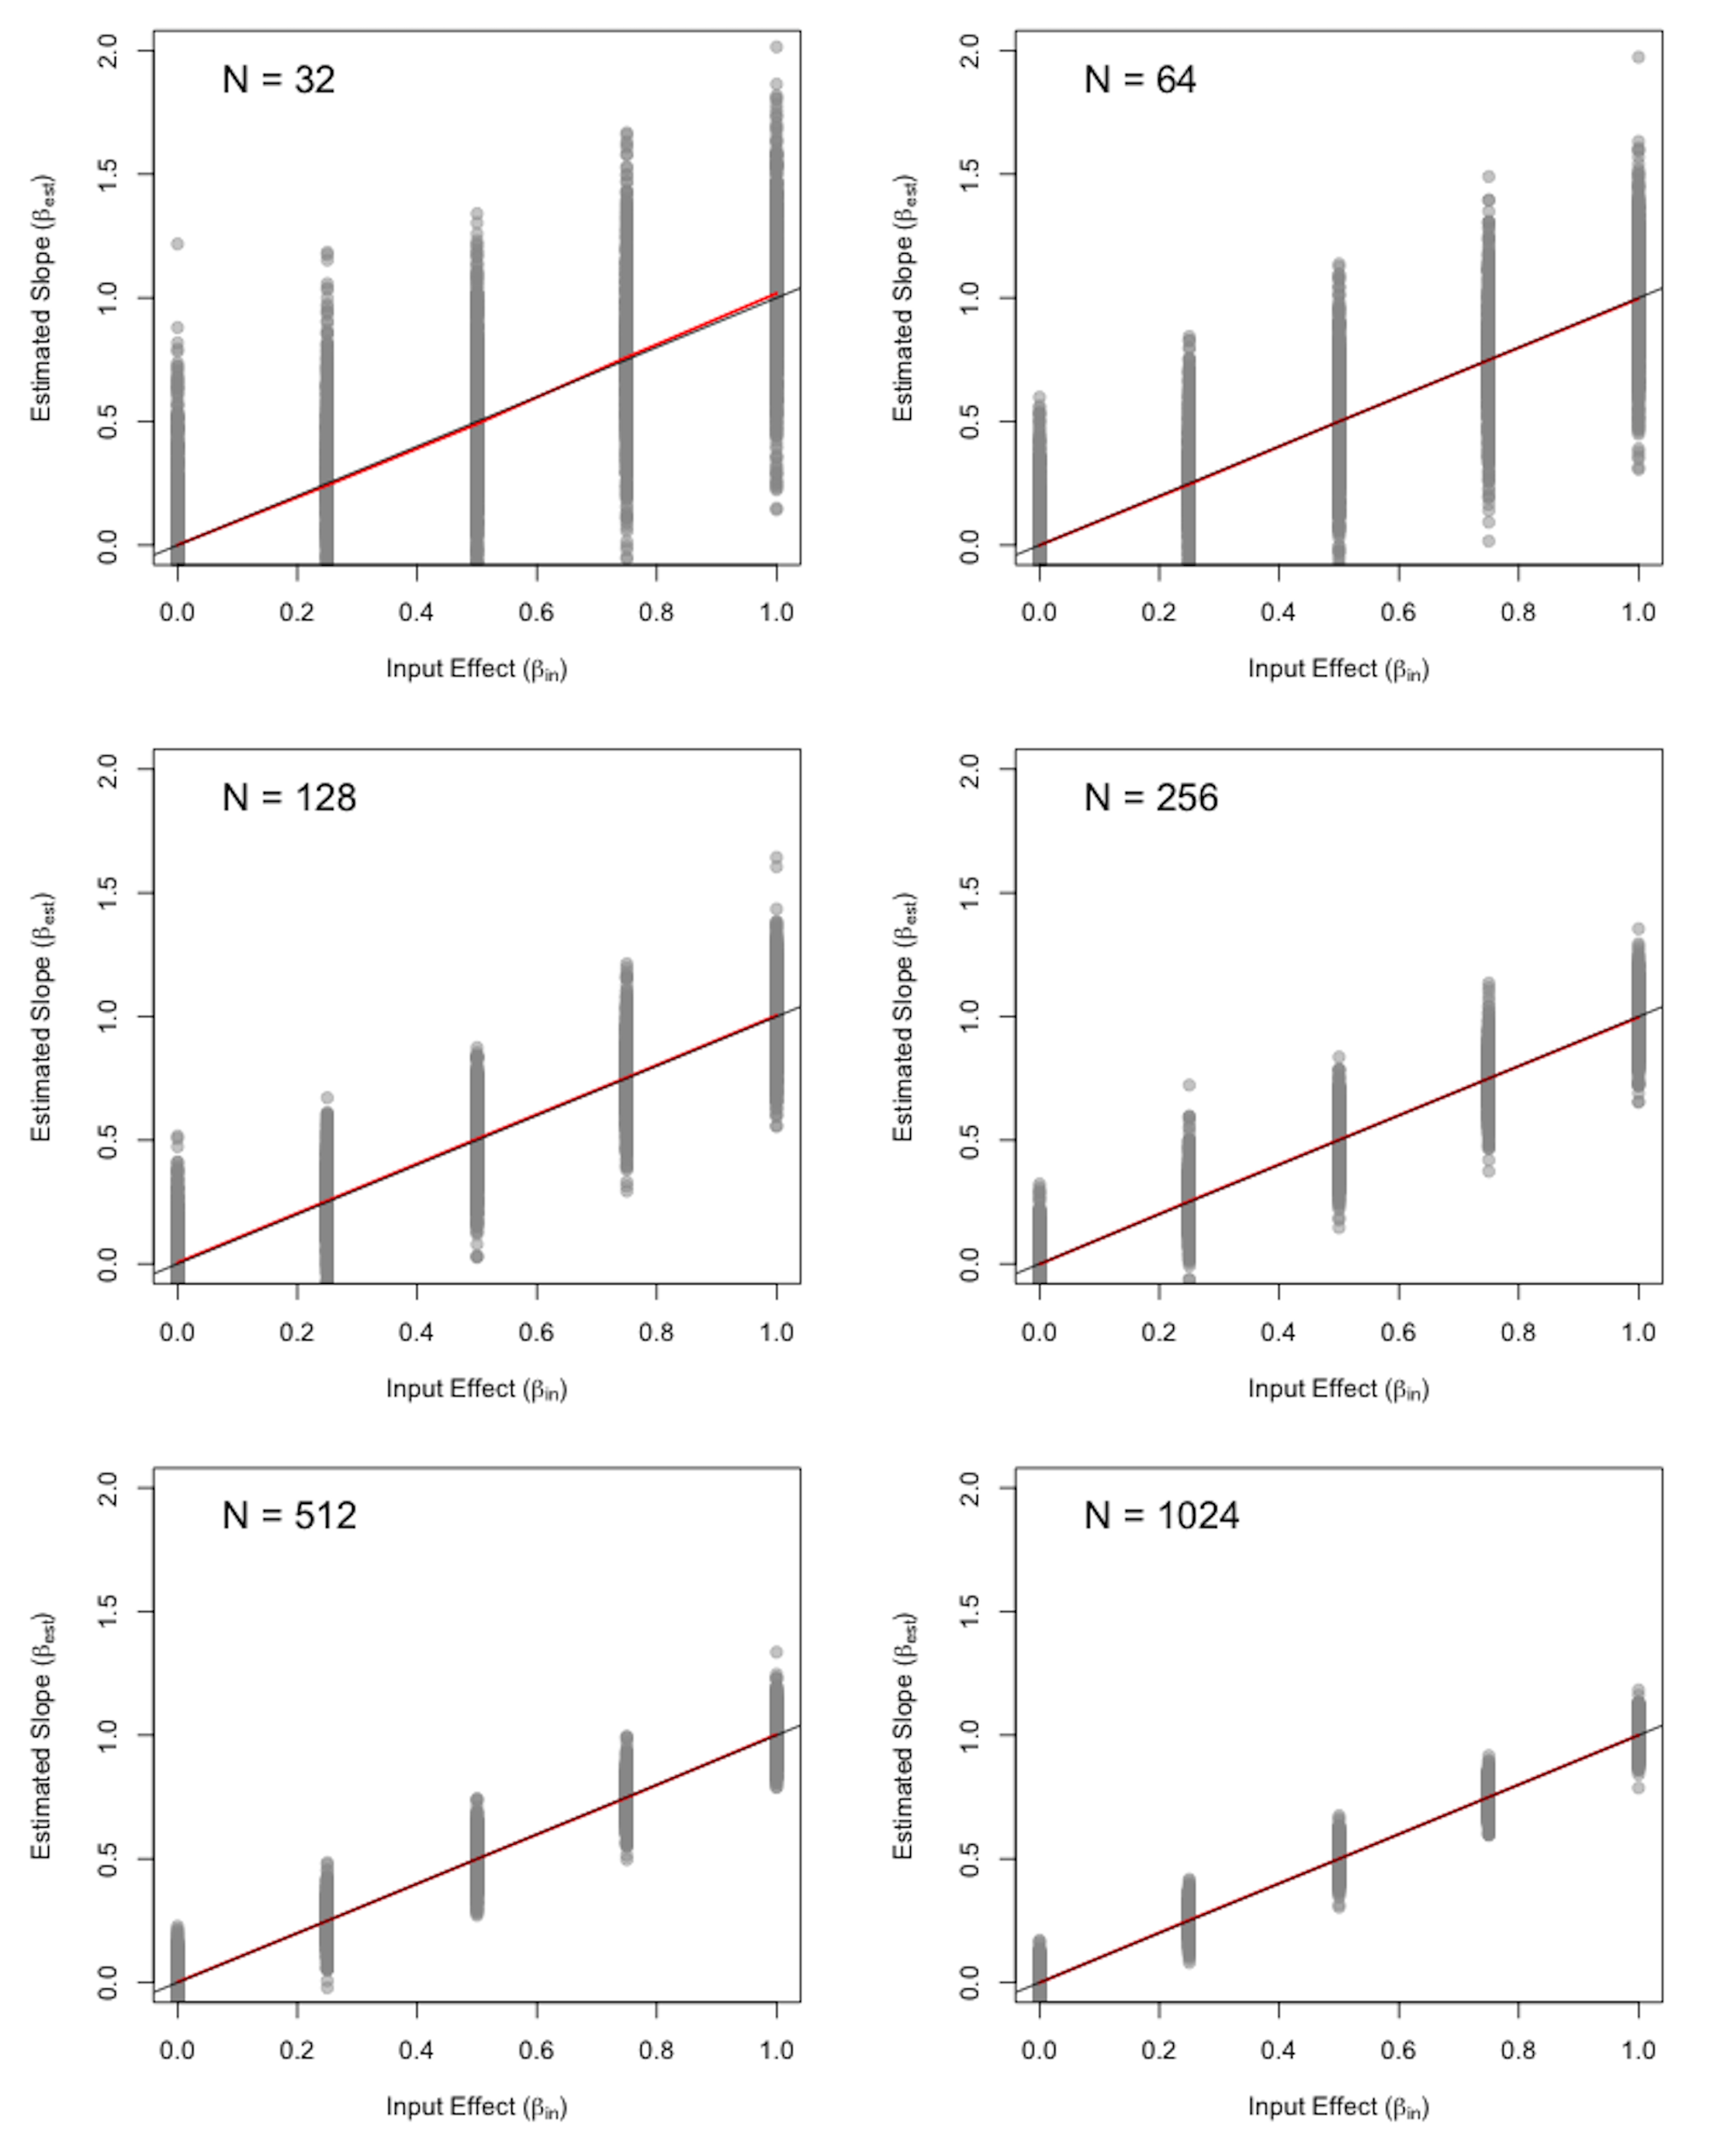
\includegraphics[width=0.95\linewidth]{fig.S18}

\textbf{Figure S18}. Parameter estimates from phylogenetic ANOVA
(incorporating \(\lambda\)). The red line represents the estimated
slope, which almost completely overlaps the gray 1:1 line.

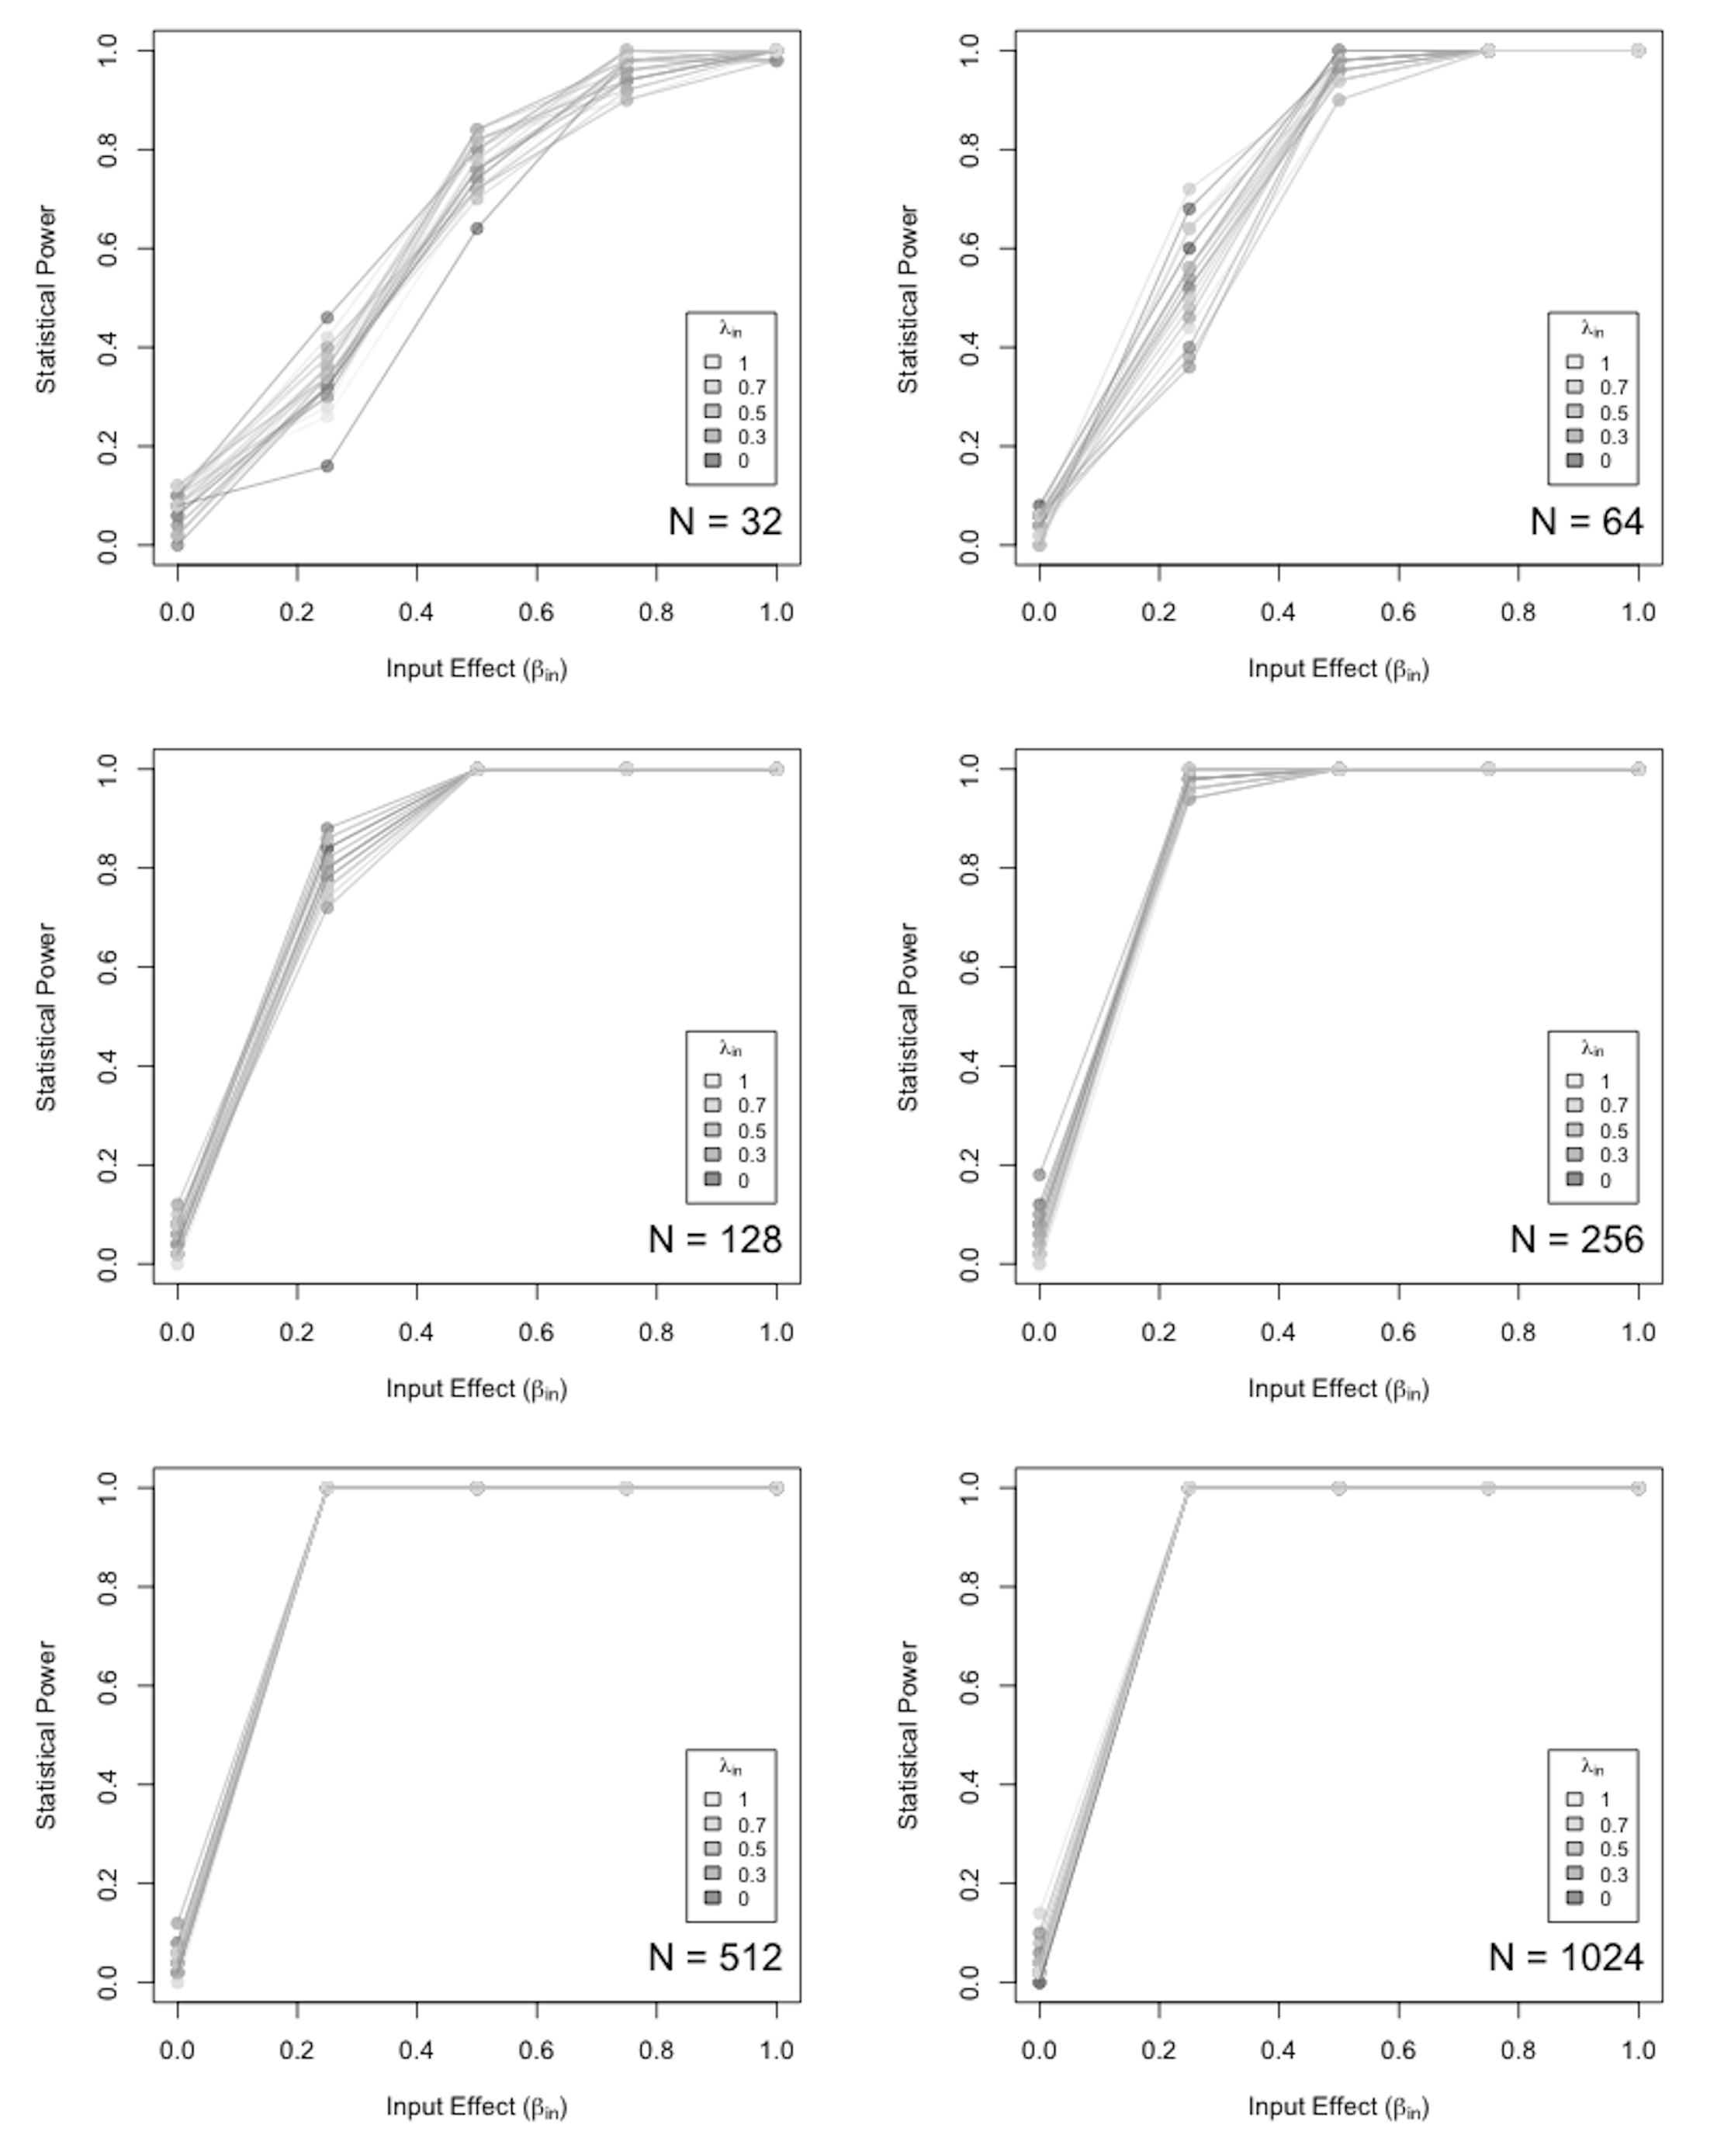
\includegraphics[width=0.95\linewidth]{fig.S19}

\textbf{Figure S19}. Power curves for phylogenetic regression
(incorporating \(\lambda\)). Type I error is found on the far-left of
the plot (effect = 0).

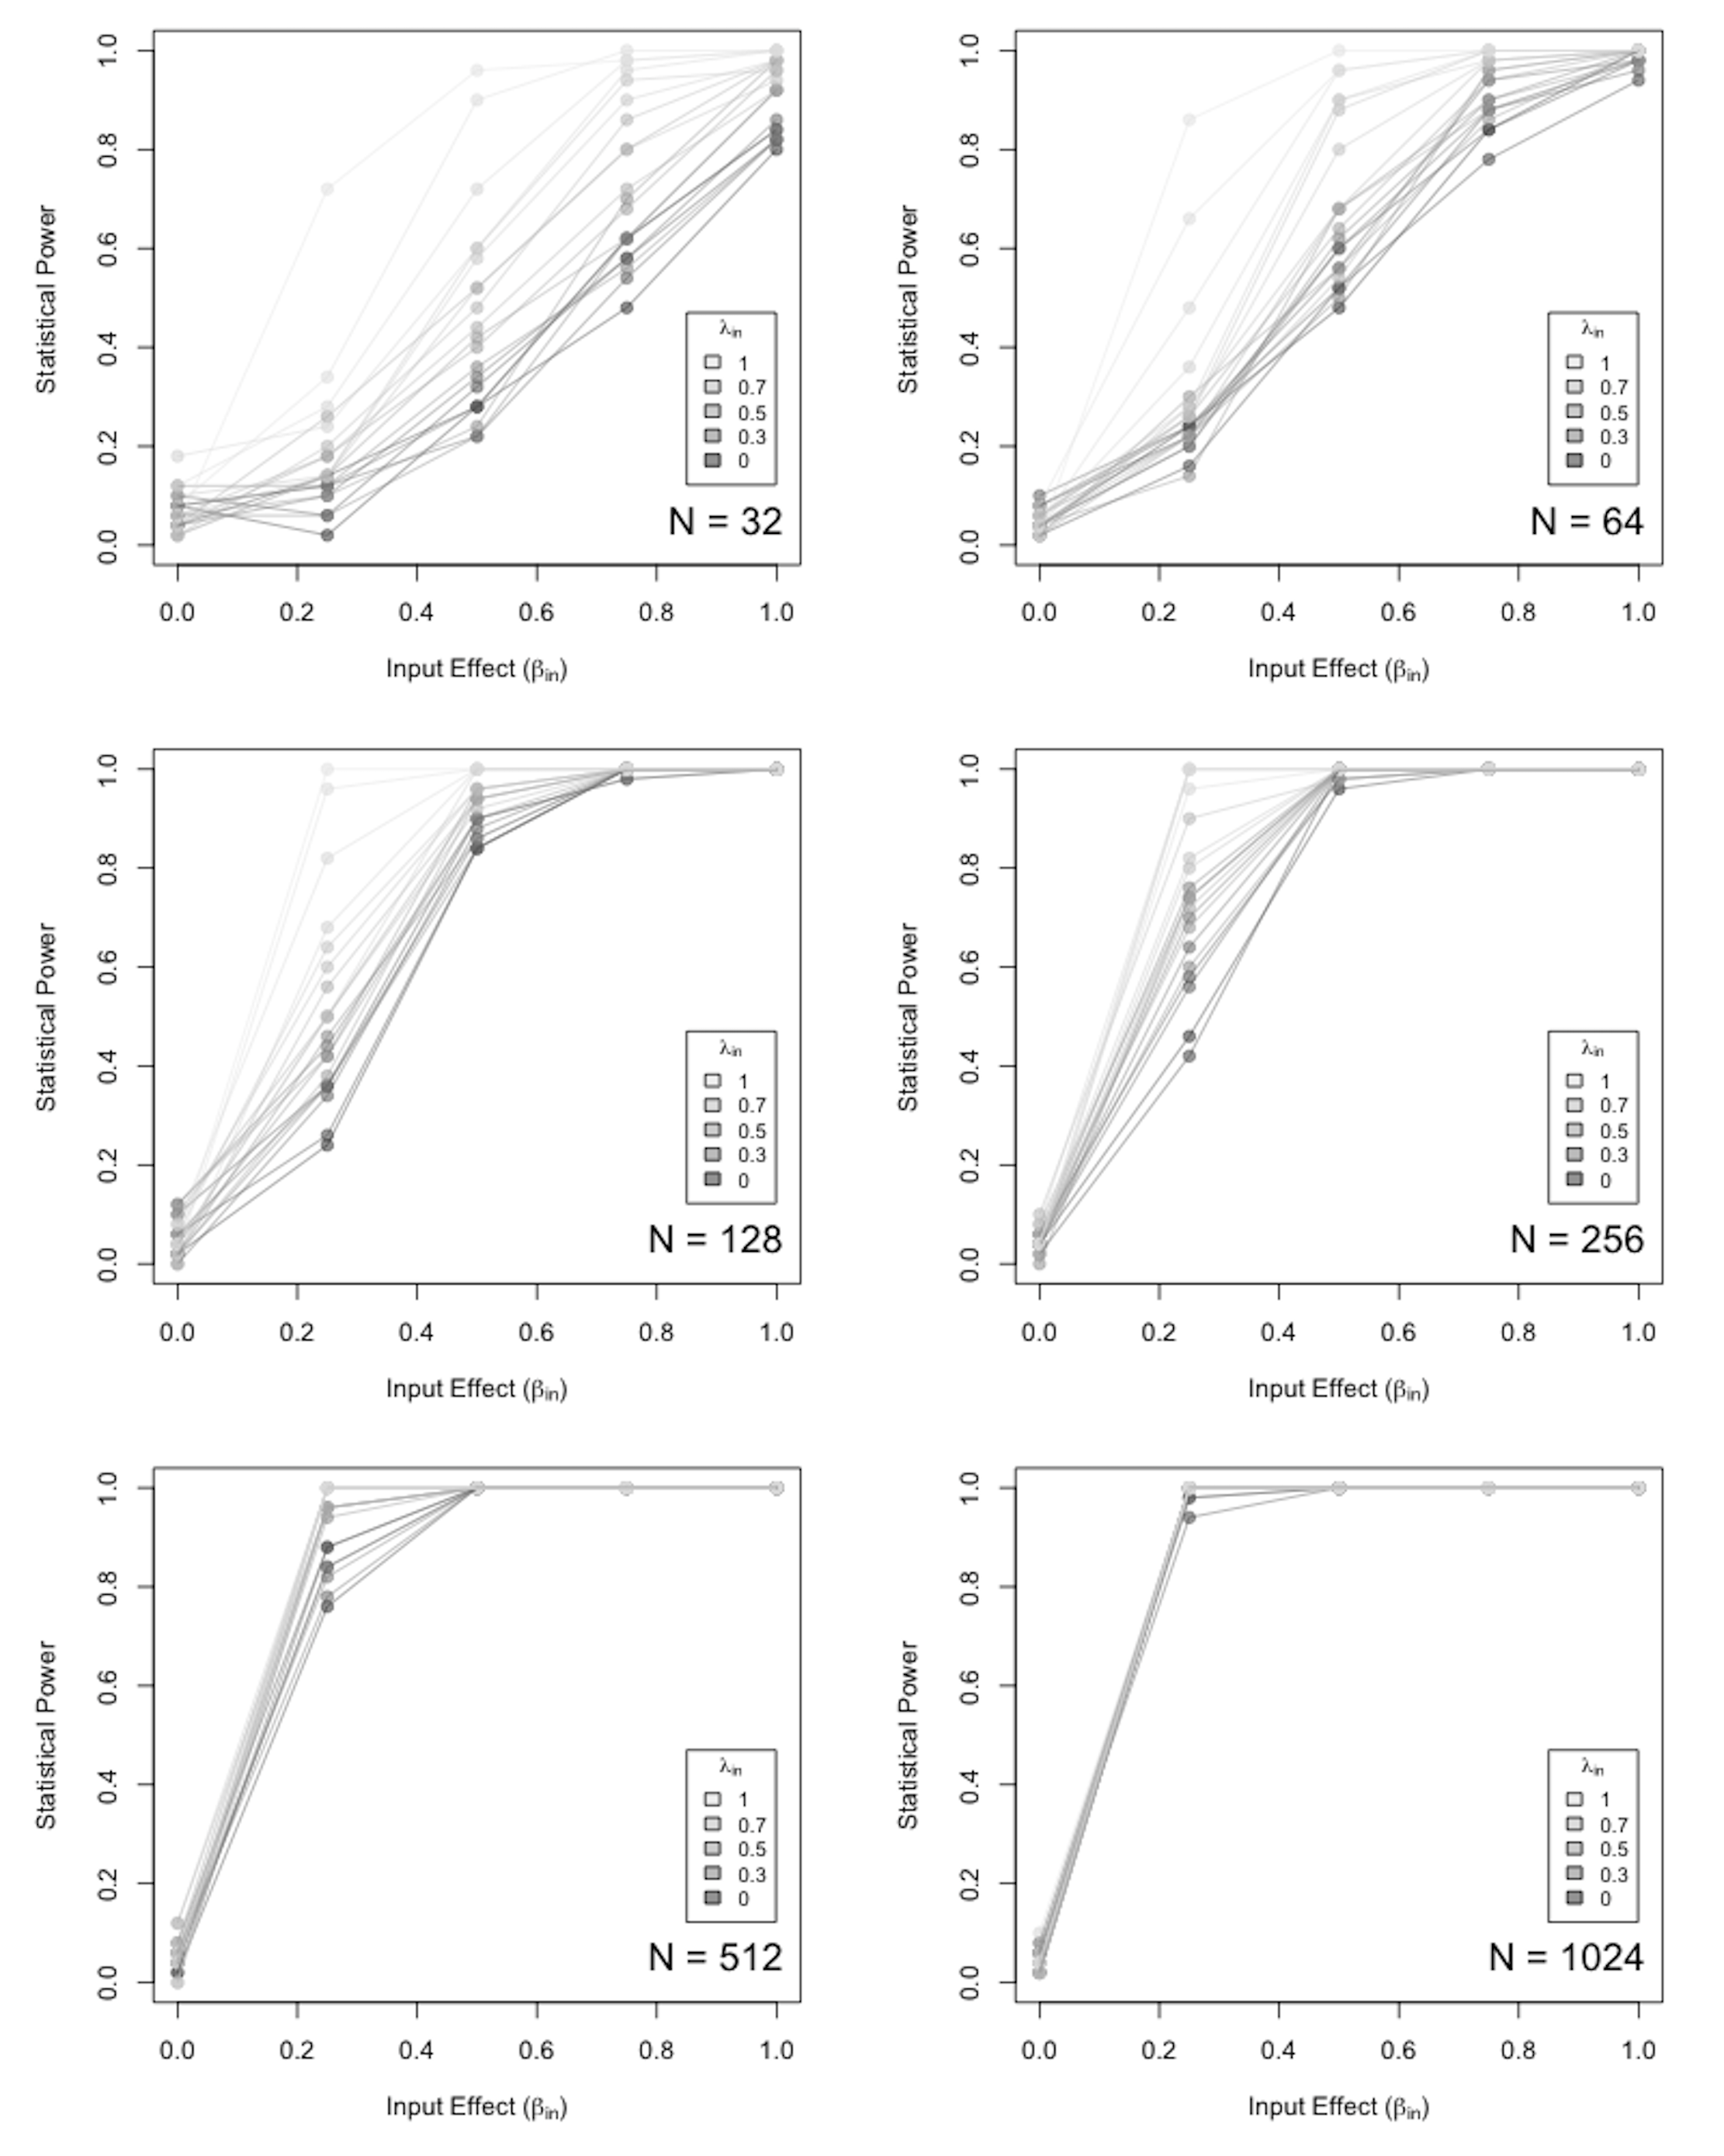
\includegraphics[width=0.95\linewidth]{fig.S20}

\textbf{Figure S20}. Power curves for phylogenetic ANOVA (incorporating
\(\lambda\)). Type I error is found on the far-left of the plot (effect
= 0).

\newpage

\hypertarget{statistical-properties-of-hatz_12}{%
\subsection{\texorpdfstring{Statistical properties of
\(\hat{Z}_{12}\)}{Statistical properties of \textbackslash hat\{Z\}\_\{12\}}}\label{statistical-properties-of-hatz_12}}

Here we examine the statistical properties of tests for comparing the
relative strength of phylogenetic signal, using \(\hat{Z}_{12}\).
Simulations were performed using pure-birth trees of different sizes
(\(n=2^5, 2^6, \cdots, 2^{10}\)), and with differing levels of
phylogenetic signal (\(\lambda=0.0, 0.5, \cdots, 1.0\)). For each
combination of \(n\) and \(\lambda\), 2 pure-birth trees were generated
and 50 traits were simulated on each phylogeny under a Brownian motion
model of evolution. Next, the phylogenetic signal between traits was
compared in pairwise fashion for all \(50*49/2 = 1225\) combinations,
using \(\hat{Z}_{12}\). The proportion of significant results provided
an estimate of the type I error or model misspecification. Specifically,
type I error was evaluated when traits were simulated using no input
phylogenetic signal (i.e., \(\lambda = 0\)). Likewise, model
misspecification was evaluated for data simulated with some known, but
equal, level of phylogenetic signal (i.e., \(\lambda > 0\)).
\hfill\break

\textbf{Results:} Tests revealed that across simulation conditions, the
average type I error of \(\hat{Z}_{12}\) was approximately 0.05 (Fig.
S21). Likewise, levels of misspecification were also low, and were at or
below the nominal 5\% level (Fig. S21 black line). Both results
demonstrate that comparisons of the strength of phylogenetic signal
using \(\hat{Z}_{12}\) do not display high levels of false positives,
and are thus appropriate for comparing the degree of phylogenetic signal
across traits.

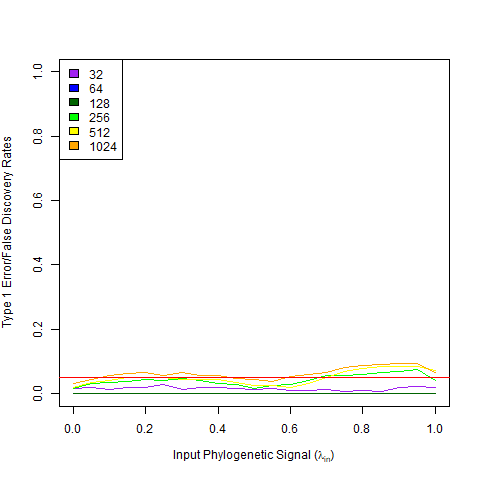
\includegraphics[width=6.67in,height=0.5\textheight]{fig.S21}

\textbf{Figure S21}. Type I error rates and model misspecification for
\(\hat{Z}_{12}\). Type I error is found on the far-left of the plot
(\(\lambda = 0\)). The solid black line represents the average type I
error and false discovery rate across all levels of input signal.

\newpage

\hypertarget{references}{%
\subsection*{References}\label{references}}
\addcontentsline{toc}{subsection}{References}

\hypertarget{refs}{}
\leavevmode\hypertarget{ref-MolinaVenegas2017}{}%
1. Molina-Venegas R, Rodríguez MA (2017) Revisiting phylogenetic signal;
strong or negligible impacts of polytomies and branch length
information? \emph{BMC evolutionary biology} 17(1):53.

\leavevmode\hypertarget{ref-AdamsCollyer2018b}{}%
2. Adams DC, Collyer ML (2018) Phylogenetic anova: Group-clade
aggregation, biological challenges, and a refined permutation procedure.
\emph{Evolution} 72(6):1204--1215.

\leavevmode\hypertarget{ref-Revell2010}{}%
3. Revell LJ (2010) Phylogenetic signal and linear regression on species
data. \emph{Methods in Ecology and Evolution} 1:319--329.

\end{document}
